\documentclass[phd,electronic,oneside,twosidetoc,letterpaper,chaptercenter,parttop,lof]{byumsphd}
\usepackage[
    bookmarks=true,
    bookmarksnumbered=true,
    breaklinks=true,
    raiselinks=true,
    pdfborder={0 0 0},
    colorlinks=false,
    plainpages=false,
    ]{hyperref}

% This makes hyperlinks point to the tops of figures, not their captions
\usepackage[all]{hypcap}

% These packages allow the bibliography to be sorted alphabetically and allow references to more than one paper to be sorted and compressed (i.e. instead of [5,2,4,6] you get [2,4-6])
\usepackage[numbers,sort&compress]{natbib}

% allow import of papers as chapters in their final pdf form. 
\usepackage{pdfpages} 

% Bar chart drawing library
\usepackage{pgfplots} 
\pgfplotsset{compat=1.18}

\usepackage{siunitx}
\sisetup{output-exponent-marker=\ensuremath{\mathrm{e}}}
\def\BibTeX{{\rm B\kern-.05em{\sc i\kern-.025em b}\kern-.08em
    T\kern-.1667em\lower.7ex\hbox{E}\kern-.125emX}}

\pgfplotsset{
/pgfplots/my legend/.style={
legend image code/.code={
\draw[thick,red](-0.05cm,0cm) -- (0.3cm,0cm);%
   }
  }
}

\usepackage{color}
\definecolor{skirretgreen}{rgb}{0.68, 0.189, 0.50}
\definecolor{mazarineblue}{rgb}{0.39, 0.60, 0.117}
\definecolor{chainganggray}{rgb}{0.113, 0.128, 0.147}
\definecolor{airforceblue}{rgb}{0.36, 0.54, 0.66}
\definecolor{beaublue}{rgb}{0.74, 0.83, 0.9}
\definecolor{dimgray}{rgb}{0.41, 0.41, 0.41}
\definecolor{darkmidnightblue}{rgb}{0.0, 0.2, 0.4}


\newcolumntype{P}[1]{>{\centering\arraybackslash}p{#1}}
\newcolumntype{M}[1]{>{\centering\arraybackslash}m{#1}}

% allow full bibliography entries to appear in the main document. 
\usepackage{setspace}

\usepackage{bibentry}
% \nobibliography*

\usepackage{tcolorbox}
\tcbuselibrary{most}

\usepackage[ruled,vlined]{algorithm2e}
\usepackage{amsmath}
\DeclareMathOperator*{\argmax}{argmax}  % In preamble

\usepackage{booktabs}
\usepackage{multirow}

\usepackage{graphicx, subcaption}

\usepackage{listings}
\usepackage{xcolor} % Optional, for styling

\lstdefinestyle{mypromptstyle}{
  basicstyle=\ttfamily\footnotesize,   % Smaller font
  lineskip=-1pt,                       % Reduces extra line spacing
  aboveskip=4pt,
  belowskip=4pt,
  showstringspaces=false,
  breaklines=true,
  breakindent=0pt,
  frame=none,
  rulecolor=\color{black},
  % literate={`}{\`{}}{1}
  % xleftmargin=1em,
  % xrightmargin=1em,
  % framexleftmargin=1em,
}
\usepackage[utf8]{inputenc}   % Enables UTF-8 encoding
\usepackage[T1]{fontenc}      % Ensures proper rendering of accented characters
\usepackage{upquote}

\def\sentimentcontroltestaccuracy{56.75\%}

% \usepackage{algorithm}
\usepackage[noend]{algpseudocode}
\usepackage{amsfonts}       % blackboard math symbols




% Because I use these things in more than one place, I created new commands for
% them.  I did not use \providecommand because I absolutely want LaTeX to error
% out if these already exist.
\newcommand{\Title}{Methods for Controlling and Evaluating Large Language Models for Creative Domains}
\newcommand{\Author}{Robert Kenneth Morain}
\newcommand{\GraduationMonth}{June}
\newcommand{\GraduationYear}{2025}

% Set up the internal PDF information so that it becomes part of the document
% metadata.  The pdfinfo command will display this.
\hypersetup{%
    pdftitle=\Title,%
    pdfauthor=\Author,%
    pdfsubject={PhD Dissertation, BYU CS Department: %
                Degree Granted \GraduationMonth~\GraduationYear, Document Created \today},%
    pdfkeywords={BYU, thesis, dissertation, LaTeX},%
}

% Rewrite the itemize, description, and enumerate environments to have more
% reasonable spacing:
\newcommand{\ItemSep}{\itemsep 0pt}
\let\oldenum=\enumerate
\renewcommand{\enumerate}{\oldenum \ItemSep}
\let\olditem=\itemize
\renewcommand{\itemize}{\olditem \ItemSep}
\let\olddesc=\description
\renewcommand{\description}{\olddesc \ItemSep}

% Important settings for the byumsphd class.
\title{\Title}
\author{\Author}

\committeechair{Dan Ventura}
\committeemembera{Tony Martinez}
\committeememberb{Nancy Fulda}
\committeememberc{Porter Jenkins}

\yearcopyrighted{\GraduationYear}

\documentabstract{I'm in.Abstract goes here.}

\documentkeywords{%
    language model, controllablity, knowledge
}

\acknowledgments{For Emi, Rosie, and Forrest.}

\department{Computer~Science}
\graduatecoordinator{Xinru Page}
\collegedean{Grant Jensen}
\collegedeantitle{Dean}

% Customize the name of the Table of Contents section.
\renewcommand\contentsname{Table of Contents}

% Remove all widows an orphans.  This is not normally recommended, but in a
% paper dissertation there is no reasonable way around it; you can't exactly
% rewrite already-published content to fix the problem.
\clubpenalty 10000
\widowpenalty 10000

% Allow pages to have extra blank space at the bottom in order to accommodate
% removal of widows and orphans.
\raggedbottom

% Produce nicely formatted paragraphs. There is nothing additional to do.  In
% case you get some problems, surround your text with
% \begin{sloppy} ... \end{sloppy}. If that does not work, try
% \microtypesetup{protrusion=false} ... \microtypesetup{protrusion=true}
\usepackage{microtype}

\begin{document}

% Produce the preamble
\microtypesetup{protrusion=false}
\maketitle
\microtypesetup{protrusion=true}

\chapter{Introduction} 
\label{chap:intro}

Creativity lies at the heart of human intelligence.
Wiggins observes that “the zenith of human intelligence is often portrayed as the ability to create…radically new and/or surprising things” and argues that creativity should be “a primary determiner of human intelligence” \cite{wiggins2006}.
This is evidenced by the role human creativity plays in society by enabling artistic expression, generating new ideas, and solving complex problems across domains such as science, mathematics, and engineering.
While the personal and subjective nature of creativity makes it difficult to define in precise cognitive or scientific terms \cite{boden1990creativity,Cskszentmihlyi1996CreativityFA,wiggins2006creativity,Simonton2018DefiningCD}, it remains universally recognized and deeply valued as fundamental to the human experience.

In computer science, the artificial intelligence (AI) research community attempts to develop machines capable of emulating human intelligence.
Through machine learning, models can process data and perform well-defined tasks, many of which were once considered exclusive to humans.
While the methods for achieving these goals have evolved \cite{Schmidhuber2022AnnotatedHO}, the fundamental ambition of the AI research community remains to develop systems that approach or surpass human-level intelligence across a wide range of tasks.

Recently, advancements in AI technologies including large language models (LLMs) like ChatGPT \cite{chatGPT} are rapidly reshaping modern life, including how people work, communicate, learn, and express themselves \cite{Gowda2023ArtificialII}. 
While this era of rapidly emerging technology is ongoing and the future consequences remain uncertain, it is clear that lasting societal change is inevitable.
However, given the far-reaching impact AI is poised to make on society, it is crucial to guide this technology's development toward the correct goals. 

While creativity is essential to human and artificial intelligence, its subjective nature poses unique challenges for AI.
Unlike more traditional AI tasks that possess well-defined objectives, creative tasks often rely on measures of inherently subjective creative attributes such as quality, novelty, typicality, and surprise \cite{ritchie07,pease2011face,jordanous2012standardised,bown2014,lamb2015,ventura2016mere,carnovalini2021,peeperkorn2023}. 
Because machines lack the same level of human experience that comes from embodiment, generating artifacts aligned with human preferences is particularly difficult for machines. 
Yet despite these challenges, the use of AI for creative purposes has grown significantly. 
Today, people use AI to generate images \cite{ho2020denoising}, music \cite{Agostinelli2023MusicLMGM}, poetry \cite{Ormazabal2022PoeLMAM}, stories \cite{Fan2018HierarchicalNS}, and more.

The computational creativity (CC) research community is dedicated to developing autonomous creative systems and creativity support tools \cite{ventura2017howto}.
Topics include CC systems, evaluation methods, co-creative systems, and philosophical questions about the nature and limits of machine creativity.
Systems developed in this domain include those that generate jokes, paintings, recipes, short stories, and other creative artifacts.
This dissertation also centers on language models, which are foundational to much of the recent progress in AI.
A language model represents the structure of a language and can be used to perform various linguistic tasks.
Formally, a statistical language model estimates the probability of a sequence of tokens, often via the chain rule:

\[
f(X_n) = \prod_{t=1}^{n} p(x_t \mid x_{<t})
\]

Early models such as n-grams and Markov chains evolved into neural approaches like LSTMs, and eventually into transformer-based architectures, which support large-scale parallelization and scaling.
Transformers have since been trained to follow instructions and generate responses aligned with human preferences. 

LLMs are viewed by many as a critical path toward achieving artificial general intelligence (AGI) systems that rival or exceed human-level performance across a wide array of intellectual and creative domains \cite{Morris2023PositionLO}. 
The emergence of these models raises pressing questions about their capacity for general intelligence and for creativity. 
This dissertation aims to contribute to the broader pursuit of artificial general intelligence by proposing methods to improve and evaluate the creative capabilities of LLMs. 
This raises fundamental questions about the purpose of developing creative AI. 
While some fear that creative AI could diminish human uniqueness or reduce opportunities for personal expression, it is worth noting that creativity plays a role not only in the arts but also in fields like science, technology, and business. 
Moreover, creativity is already commodified in many domains such as marketing and Hollywood, where the artistic product is produced primarily to satisfy market demands rather than for personal satisfaction. 
In such cases, using AI to enhance or replace creative labor is not unlike automating less artistic domains such as software engineering or customer service. 
Additionally, AI can democratize creativity by lowering barriers so that anyone, regardless of artistic skill, can bring their ideas to life.

This dissertation presents a body of work which furthers the goal of developing artificial general intelligence through a principled approach for improving and evaluating the creative capabilities of LLMs. 
Accordingly, the chapters of this dissertation fall into two broad categories: model development and frameworks (Chapters \ref{chap:ssm}–\ref{chap:llmexica}), and evaluation and analysis (Chapters \ref{chap:chatgpt_for_cc}–\ref{chap:cc_prompting}).

Chapter \ref{chap:ssm} addresses a fundamental limitation of LLMs in storing parametric knowledge, introducing an external knowledge retrieval mechanism inspired by symbolic memory in human cognition. 
Drawing from psychological models where concepts are organized as structured graphs with nodes and edges, this approach enables the integration of structured semantic data into a causal language model. 
By offloading knowledge storage to external mechanisms, the model's parameters are freed to focus on modeling other linguistic features and enables more control over the symbolic reasoning ability of the model for traditional and creative tasks. 

Chapter \ref{chap:bbc} addresses the challenge of controlling LLMs in black-box settings where users access models through APIs and web interfaces that restrict internal model features. 
This chapter presents a reward-driven prefix conditioning method that trains a controller model to generate control prefixes based on control instructions and prompts, enabling users to influence model behavior without requiring internal parameter access. 
These methods demonstrate comparable performance to traditional white-box approaches and are general to a wide variety of tasks that can be described with rewards, including creative tasks.

Chapter \ref{chap:codenames} presents a framework for creative agent development based on the game Codenames, addressing the inherent challenge of evaluating creative systems due to their subjective nature. 
Building on \citeauthor{spendlove2022competitive}'s approach of using games that require creativity for more objective evaluation, this framework provides a web interface, game server, and Python client for developing Spymaster and Guesser agents. 
Evaluation in both a computational creativity research workshop and a graduate-level course demonstrates the framework's effectiveness in enabling rapid iteration and prototyping of creative agents through the structured Codenames Spymaster task.

Chapter \ref{chap:llmexica} explores developing a symbiotic relationship between generative and symbolic AI by introducing methods for automatic knowledge base creation for narrative generation tasks. 
This work presents a pipeline that leverages an LLM to parse short stories and extract story actions along with their corresponding preconditions and postconditions. 
The pipeline is evaluated through user surveys to verify logical consistency of generated artifacts and direct analysis with error correction. 
This results reveal insights into LLM limitations in symbolic reasoning while demonstrating how generative and symbolic approaches can complement each other's creative abilities.

Chapter \ref{chap:chatgpt_for_cc} presents a comparative study evaluating ChatGPT's performance against bespoke, domain-specific traditional CC systems to determine how successful general models are relative to specialized approaches.
Results show that ChatGPT outperformed traditional CC systems across all domains, raising important questions about the utility of domain-specific systems while also revealing areas where LLMs still have room for improvement in creative tasks.

Chapter \ref{chap:cc_prompting} presents a comparative study of representative prompting methods to measure the effect of algorithmically complex techniques on LLM-generated creative artifacts across multiple domains (jokes, poems, six-word stories, flash fiction). 
The analysis reveals that advanced prompting techniques such as OPRO and chain-of-thought prompting surprisingly do not produce artifacts of significantly higher quality, novelty, or creativity than basic prompting approaches. 
These results expose limitations in LLMs' ability for automatic evaluation of creative outputs, provide empirical grounding for selecting prompting methods in creative text generation, and raise important questions about the fundamental creative limitations of large language models and prompting approaches.

In summary, creativity is a critical aspect of intelligence that requires targeted research, especially as we pursue the goal of artificial general intelligence. 
This dissertation contributes to that pursuit by proposing new tools, frameworks, and evaluation methods for modeling and assessing creativity in LLMs. 
Ultimately, creative AI has the potential not only to replicate human ingenuity, but to amplify it by enabling new forms of self-expression and idea generation that would be impossible otherwise.


\chapter{Symbolic Semantic Memory in Transformer Language Models} 
\label{chap:ssm}

I hereby confirm that the use of this article is compliant with all publishing agreements.

\

\noindent
Robert Morain, Kenneth Vargas and Dan Ventura, ``Symbolic Semantic Memory in Transformer Language Models,'' IEEE International Conference on Machine Learning and Applications, 2022, pp. 992-998, doi: 10.1109/ICMLA55696.2022.00166. 


% % Variables
\newcommand{\LMLossPercentageDecrease}{81.04\%}

% \maketitle

\begin{abstract}
This paper demonstrates how transformer language models can be improved by giving them access to relevant structured data extracted from a knowledge base. 
The methods for doing so include identifying entities in a text corpus, sorting the entities using a novel attention-based approach, linking entities to a knowledge base, then extracting and filtering the knowledge to create a knowledge-augmented dataset.
We evaluate these methods with the WikiText-103 corpus using standard language modeling objectives.
These results show that even simple additional knowledge augmentation leads to a reduction in validation perplexity by \LMLossPercentageDecrease. 
These methods also significantly outperform common ways of improving language models such as increasing the model size or adding more data.
\end{abstract}


\section{Introduction}
Currently, transformer language models are the gold standard\footnote{The top 10 models on SuperGLUE's~\cite{wang2019superglue} leaderboard are all transformer-based models} for most language tasks.
The strength of these models comes from their extensive pretraining on statistical language modeling tasks.

In recent years, many improvements have been made to transformer language models.
These improvements include adding layers and parameters \cite{brown2020language} as well as making changes to the model architecture \cite{devlin2018bert}.
There has also been work put into prompt engineering \cite{zhang2021differentiable} to help guide the model to produce some desired output.
The work presented here demonstrates a different approach aimed at improving a transformer language model's ability to access semantic information.

One problem with traditional self-supervised language modeling tasks is that semantic knowledge is only tangentially acquired.
To gain more semantic knowledge, these models typically become larger and are trained with more data.
It has been argued elsewhere that these models have no way of reasoning about the knowledge they have acquired and instead are ``haphazardly stitching together sequences of linguistic forms...observed in...vast training data, according to probabilistic information about how they combine, but without any reference to meaning'' \cite{bender2021dangers}.
This work designs simple experiments to demonstrate how language models can be improved by giving them access to additional structured data rather than strictly relying on statistics.

To proceed, we draw inspiration from research on semantic memory as a cognitive process \cite{tulving1972episodic}. 
Unlike transformer models, humans rely on their semantic and episodic memory to understand language and decide how to respond.
While there are connectionist and symbolic models for semantic memory~\cite{jones2015models}, this work loosely draws inspiration from the symbolic approach.
Also, since transformers are connectionist models already, using a symbolic model of semantic memory allows us to create a connectionist-symbolic hybrid which has proven to be effective on certain symbolic tasks~\cite{mao2019neuro}.

Another significant influence on this work comes from Daniel Kahneman's research on reasoning and decision making.
Kahneman proposes a cognitive model which distinguishes between System 1 and System 2 thinking \cite{kahneman2011thinking}. While System 1 is fast, instinctive, and emotional, System 2 is slower, more deliberative, and more logical. 
The base transformer model can loosely be compared to Kahneman's System 1 fast thinking, while knowledge base integration resembles the slower System 2.
Similar to how the SOAR cognitive architecture attempts to replicate various cognitive processes, a transformer-knowledge base hybrid seems appropriate in this case \cite{laird2012soar}.

The idea of combining connectionist and symbolic models has recently become more popular. 
Bosselut \textit{et al.} introduced Commonsense Transformers (COMET) \cite{bosselut2019comet}, a GPT-2 model trained on ATOMIC \cite{sap2019atomic} and ConceptNet \cite{liu2004conceptnet} to automatically construct knowledge graphs.
Miller \textit{et al.} introduces key-value memory networks which are trained on structured data from Wikipedia to improve performance on question answering tasks \cite{miller2016key}.
The CLEVR dataset \cite{johnson2017clevr} is a visual question answering dataset specifically designed to test a model's reasoning abilities by minimizing biases that models can exploit.
This work shares the goal of improving a model's reasoning abilities through symbolic methods.

The contributions of this paper include:
\begin{itemize}
    \item Methods for augmenting language datasets with knowledge base data including attention-based entity selection.
    \item Modification to GPT-2's causal mask to attend to additional knowledge data.
    \item Demonstrating the effectiveness of knowledge augmented data on language modeling, which reduces perplexity by \LMLossPercentageDecrease.
\end{itemize}

\section{Related Work}

There is an extensive body of research on knowledge augmented language models from which this paper takes inspiration.
REALM uses a knowledge retriever which allows a language model to attend to relevant documents from a large corpus such as Wikipedia \cite{guu2020realm}. 
While incorporating increasingly larger contexts into language models has proven to be a fruitful vein of research, Guu \textit{et al.} claim to extend this progression beyond sentences and paragraphs all the way to the corpus level. 
We follow their lead by integrating knowledge from a large knowledge source.
However, this work explores the potential of structured knowledge from a knowledge base rather than a document database.

KEPLER integrates knowledge into a language model by jointly training on language modeling and knowledge embedding objectives \cite{wang2021kepler}.
This causes the language model to build entity representations that contain an entity's description and are close to other linked entities in a knowledge base.
Here, we utilize structured knowledge without requiring auxiliary objective functions.

KALM augments a recurrent neural network \cite{liu2019knowledge} by allowing the model to sample from vocabularies collected from a knowledge base and grouped by entity type.
While KALM learns to identify entities in an unsupervised fashion, we follow the lead of models like KnowBert \cite{peters2019knowledge} which requires entity selection and linking. 
KnowBert implements a Knowledge Attention and Recontextualization
mechanism which can be added to a layer in the language model to integrate knowledge from a knowledge base.
This method combines pretrained entity embeddings with BERT-encoded token hidden states.
Unlike KnowBert, our methods utilize a single model to encode and attend to the added knowledge.

\section{Methods}

These methods outline one way to augment a text corpus with semantic knowledge.
While this process is general to any dataset or knowledge base, a description of the specific implementation details are provided.
    
\subsection{Augmented Dataset Creation}
    
\begin{figure}
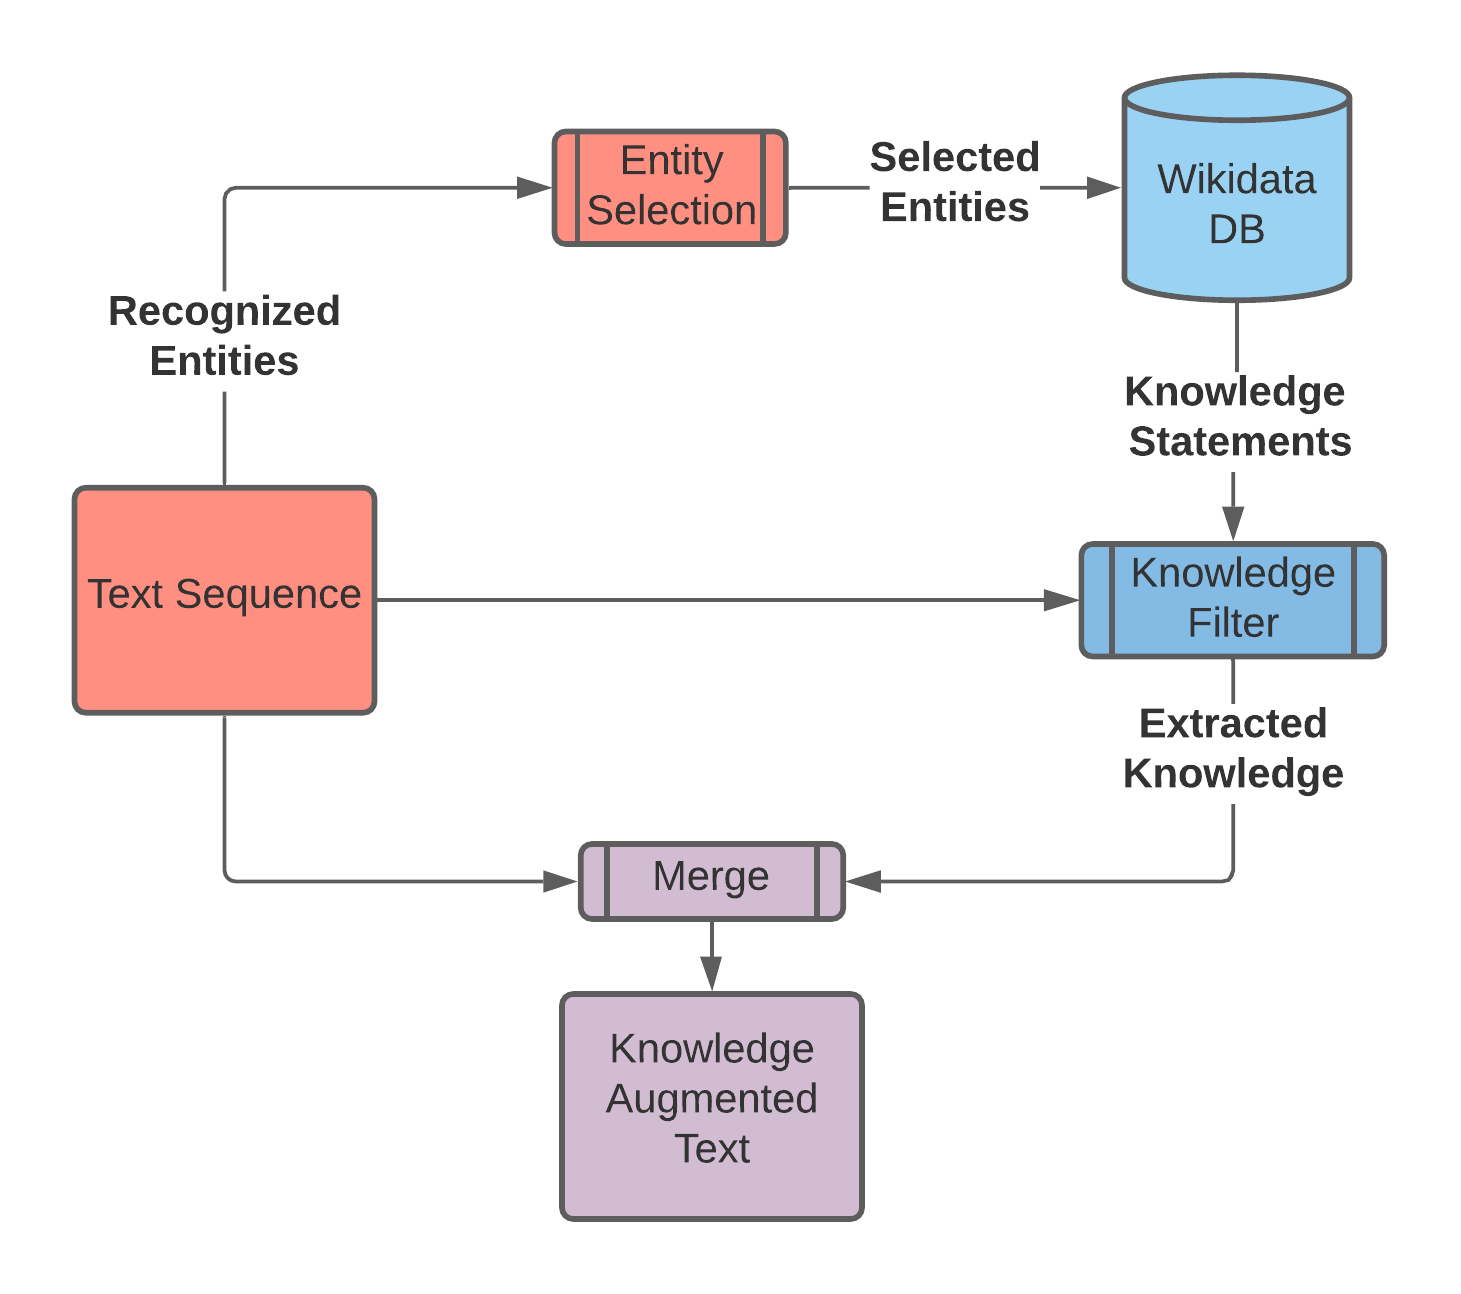
\includegraphics[width=0.5\columnwidth]{images/ssm/augmented_dataset_creation.png}
\centering
\caption[Augmented dataset creation]{
    For each sequence in a language dataset, spaCy is used to identify the entities.
    Based on the entity selection criteria, a single entity is used to query the Wikidata database to acquire a set of knowledge statements.
    These statements are then filtered based on their relevance to the corresponding sequence.
    Lastly, the knowledge for each sequence is concatenated to the end of the original text sequence. 
}
\label{fig:augmented_dataset_creation}
\end{figure}

The augmented dataset creation process is composed of a \emph{knowledge base}, an \emph{entity selection} algorithm, a \emph{knowledge extraction} process, and a \emph{merge} between the extracted knowledge and the original dataset.
Figure \ref{fig:augmented_dataset_creation} shows how these systems work together to select the supplementary data to include in the augmented dataset. 
For each sequence in the dataset, a set of entities is extracted from the sequence and filtered based on the entity selection algorithm to a single entity.
This entity is then used to query the knowledge base to return a set of knowledge statements.
The knowledge statements are filtered and the remaining statements are concatenated to the end of the original text sequence.
Once the entire dataset is augmented, it is ready to be used for training the knowledge transformer model.

\textbf{Dataset:}
The WikiText-103 dataset \cite{merity2016pointer} is used to train each of the models. 
After removing rows with no entities in the knowledge base, this dataset consists of a split with 628,965 (99.8\%) training rows and 1,320 (0.2\%) validation rows\footnote{These are standard splits from Huggingface's datasets library at \url{https://huggingface.co/datasets/wikitext}}. 
The WikiText language modeling dataset is a collection of over 100 million tokens extracted from the set of verified Good and Featured articles on Wikipedia. 
It makes sense to use this dataset for fine-tuning GPT-2 because WebText excludes Wikipedia articles from it's training dataset \cite{radford2019language}.

\textbf{Knowledge base:}
Wikidata \cite{vrandecic2014wikidata} is a free and open knowledge base of structured \cite{cafarella2011structureddata} Wikimedia data.
While there is an API to access the official version hosted by Wikidata, this approach proves to be too slow to be used on large datasets.
To reduce the time of each Wikidata query, a downloaded \href{https://dumps.wikimedia.org/wikidatawiki/entities/}{JSON data dump} of the knowledge base can be converted into a database. 
While Wikidata supports many languages, only the English entities and properties are used. 

In Wikidata, \emph{items} refer to entities in the knowledge base, including people, topics, concepts, and objects. 
For example, the ``1988 Summer Olympics'', ``love'', ``Elvis Presley'', and ``gorilla'' are all \emph{items} in Wikidata.
A \emph{statement} is defined as a relation between an \emph{item} and a \emph{value} by way of a \emph{property}. 
\emph{Statements} follow the resource description framework (subject-predicate-object) \cite{miller1998rdf}.
Generally, \emph{values} are other \emph{items} but can also be unknown or quantitative values. 

% Named entity recognition
\textbf{Attention-based Entity Selection:}
The first step in the entity selection process is to identify words in the sequence that may have items in the knowledge base. This problem can be framed as a traditional named-entity recognition task to identify predefined categories such as person names, organizations, locations, medical codes, time expressions, quantities, monetary values, percentages, etc.  For example, with the sentence ``Apple is looking at buying U.K. startup for \$1 billion'', Apple, U.K., and \$1 billion are considered entities. While there are many methods for named-entity recognition, spaCy\footnote{\url{https://spacy.io/}} is used to extract the named-entities in each sequence. 

% Entity selection
Once a set of entities are identified in a text sequence, a single entity is included in the augmented dataset based on the entity selection criteria. 
In these experiments, an entity's average attention score is determined by inputting a sequence of text into a pretrained GPT-2 small model and returning the attention scores for each model layer.
These attention scores are then averaged across layers, heads, sequence, and entity tokens---resulting in a single attention score for each entity in the sequence.
These entities are then sorted by their (averaged) attention score to determine the maximum, median, and minimum attention-score entity.
We interpret this ordering of entities to indicate their relative importance as determined by GPT-2 in the context of the input sequence.
Figure \ref{fig:attention_scores} provides more details about how these attention scores are calculated.

\begin{figure}
    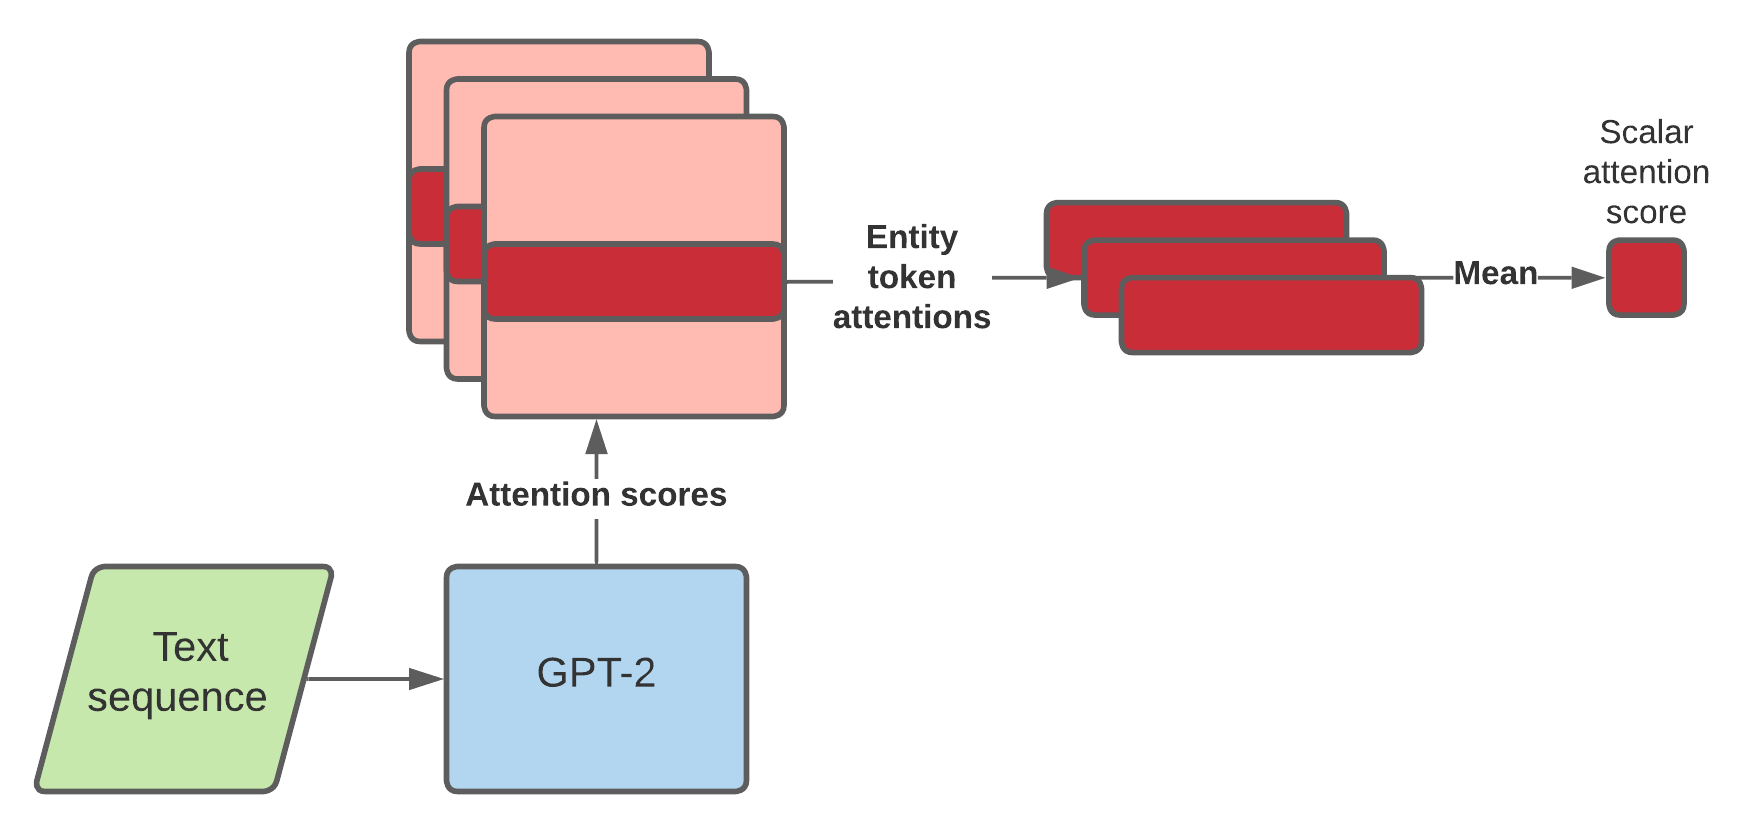
\includegraphics[width=0.75\columnwidth]{images/ssm/attention_score_calculation.png}
    \centering
    \caption[Attention score calculation]{
        To compute an entity-specific score: a sequence is input to a pretrained GPT-2 model and the token attention scores are returned in an 
        $n\times n\times h$
        tensor, where $n$ is the sequence length and $h$ is the number of heads;   
        the scores of each entity are isolated by selecting only the rows corresponding to the tokens of the entity in question; the scores are averaged across heads, the sequence length, and the entity tokens.
        The result is a single average attention score value for each entity in the sequence. 
        This allows the entities to be sorted by their average attention score.
    }
    \label{fig:attention_scores}
\end{figure}

% Knowledge extraction 
\textbf{Knowledge Extraction:}
In general, the knowledge extraction process consists of querying the knowledge base for information and then filtering that information based on the input sequence. 
For these experiments, all of the knowledge is filtered out except for the description of the entity. 
This information is recorded in JSON format like so: \emph{\{label : description\}}.

While this knowledge extraction process is simple, the purpose of this work is not to optimally select the best possible knowledge for a given input sequence. 
For now, it is sufficient to show that even naive semantic data can improve performance on language tasks.
The task of developing more sophisticated knowledge extraction methods is left to future work.

\textbf{Merge:}
The augmentation process is complete once the extracted knowledge is combined with the original dataset. 
This is done by concatenating the knowledge text to the end of the input text.
        
    
\section{Experiments}

The knowledge augmentation process is evaluated on a language modeling task.
Since a language model is often indirectly asked to exploit the semantic knowledge it has acquired through pre-training, it stands to reason that language modeling would benefit from adding supplementary knowledge to the dataset.

\subsection{Knowledge-augmented Language Modeling}

This section describes the details for handling a language modeling task with additional semantic knowledge added to the dataset.
While modifications to a model's architecture are not always necessary, some changes may be required to allow the model to exploit this added knowledge.

\subsubsection{Knowledge Model}

GPT-2 is used as the base model for causal language modeling on each knowledge augmented dataset. 
The causal mask of Huggingface's \cite{wolf2019huggingface} implementation of the standard GPT-2 architecture must be modified to allow the model to attend to the knowledge tokens at the end of the input (see Figure~\ref{fig:knowledge_model}).
        
\begin{figure}
    \centering
    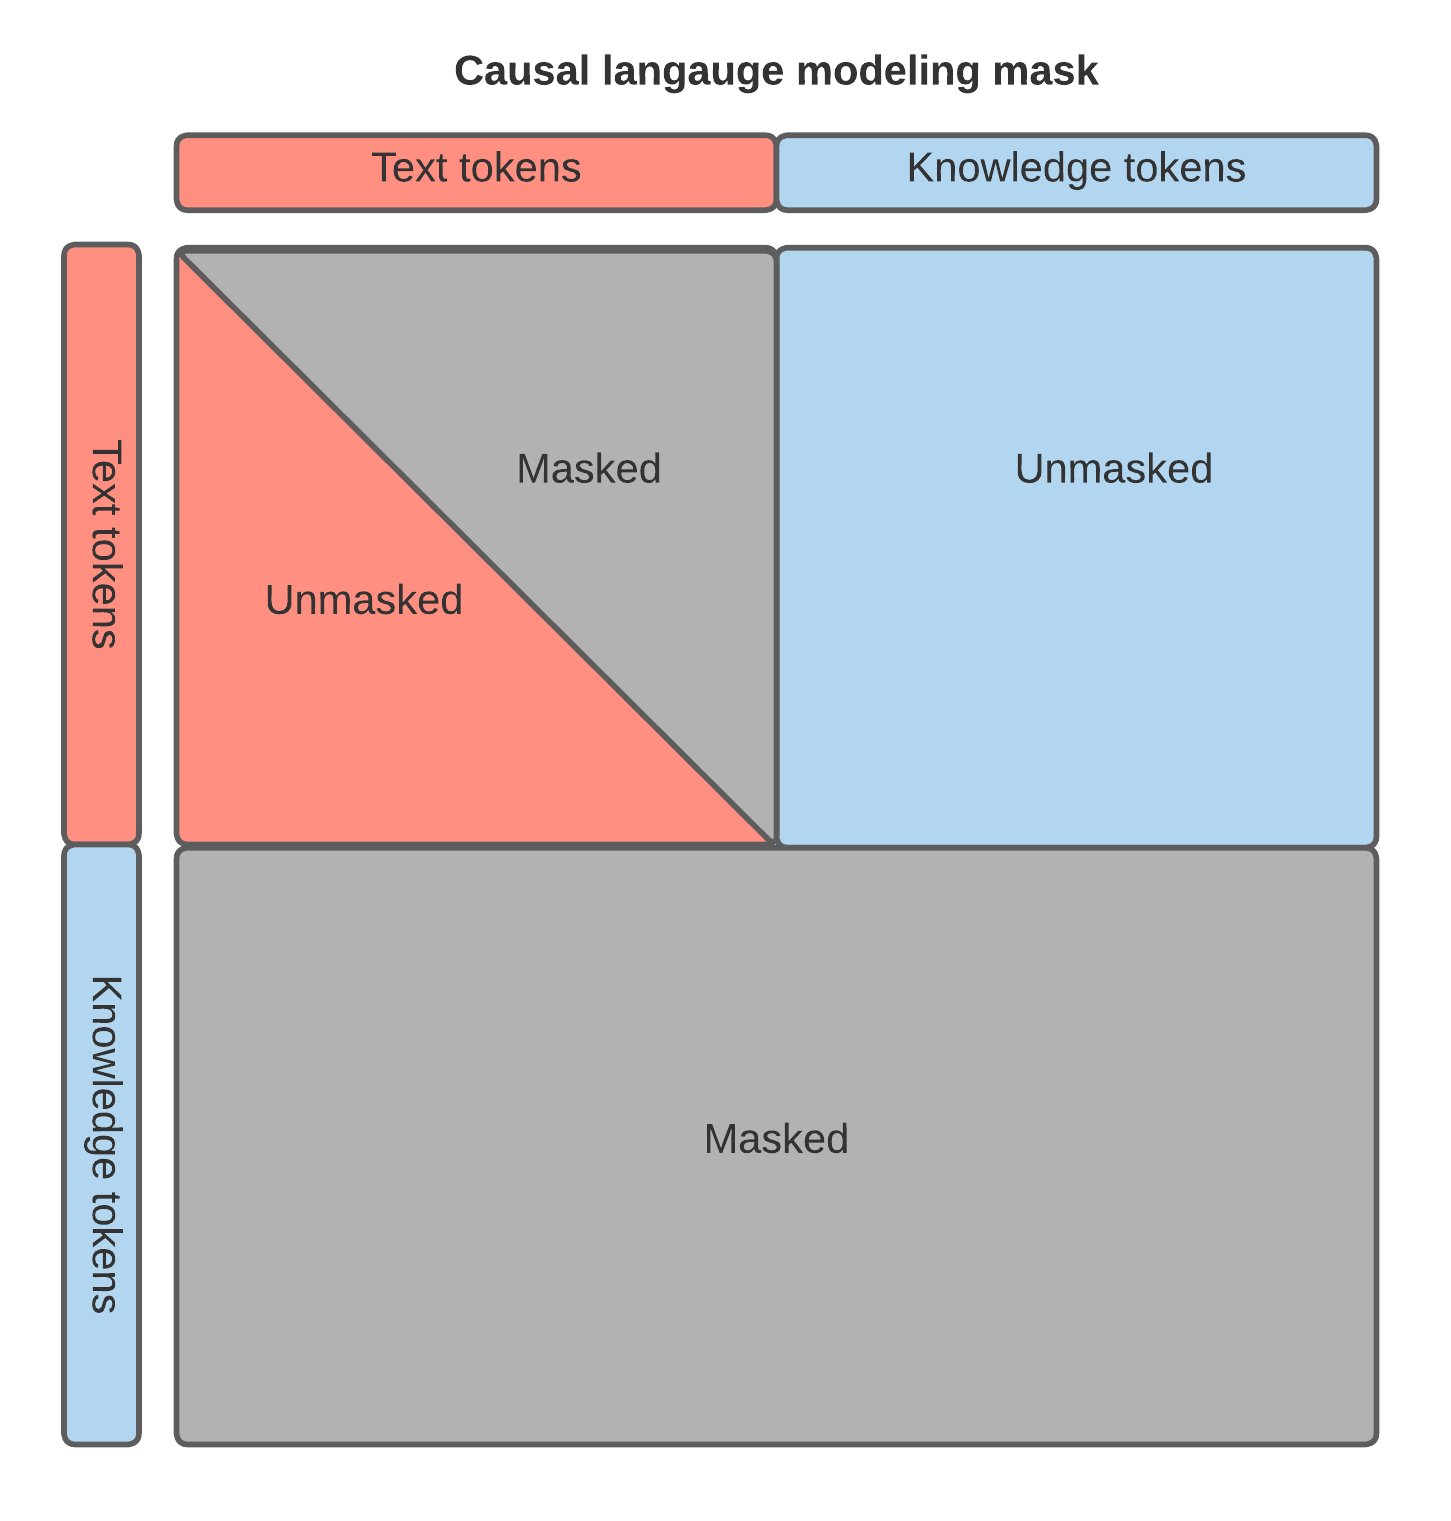
\includegraphics[width=0.5\linewidth]{images/ssm/knowledge_model_causal_mask.png}
    \caption[Knowledge model causal mask]{
        Modifications to the causal mask of Huggingface's GPT-2 to allow the text tokens to attend to knowledge tokens for each prediction.
        Recall that attention scores are calculated from each token to every token in the sequence, resulting in an $n \times n$ attention matrix.
        The text tokens are masked normally, with one less token being masked for each row until all but one of the tokens is unmasked (upper left quadrant).
        In the upper right quadrant, all of the knowledge tokens are unmasked to allow each unmasked text token to attend to the knowledge tokens.
        Since the model does not predict on the knowledge tokens, all tokens are masked on the lower half of the causal mask.
    }
    \label{fig:knowledge_model}
\end{figure}
        
While the text tokens are masked normally, the knowledge tokens are always attended to.
One could argue that this gives an unfair advantage to the knowledge model over the baseline GPT-2 model because the added tokens bias the model early on in the sequence.
First of all, we argue that this bias is a good thing because it more closely resembles how a human might rely on their semantic memory while reading or listening.
In spite of this, these results include experiments with a smaller, filtered dataset where additional contiguous text populates the knowledge tokens buffer (a sliding window over the entire dataset is not used).
This filtered dataset only consists of rows that have excess knowledge tokens (333,753 train, 877 validation). 
Comparing this dataset with an identical dataset where knowledge tokens fill the knowledge buffer considers the benefit of added semantic knowledge vs. the benefit of additional textual context.
We also include results using an attention mask which eliminates entity leakage from the added knowledge.

\subsubsection{Baseline}

The baseline for this experiment is an unmodified pretrained GPT-2 small model fine-tuned on the WikiText dataset.
This is sufficient to observe the effect that additional knowledge has on language modeling.
All of the models are trained using a batch size of 32, a learning rate of \num{1e-4}, and the ADAM optimizer \cite{kingma2015adam}.
The early stopping criteria terminates training after three epochs of no improvement to the validation perplexity.
The length of the text sequence is limited to 128 tokens while leaving a 64 token buffer available for knowledge tokens.
        
\subsubsection{Entity Selection Criteria}

These experiments focus on three primary variations of entity selection.
As discussed previously, the average attention score for each entity is calculated using the attention scores output by a pretrained GPT-2 model (Figure~\ref{fig:attention_scores}).
Given a list of entities ordered by attention score, the performance when using the maximum-, median-, or minimum-attention score as the entity selection criterion is compared. Based on which entity is selected, the corresponding description is retrieved from the knowledge base to form a knowledge statement.
This knowledge statement populates the knowledge buffer as described previously.
The four possible combinations of these primary variations (max/median, max/min, median/min, max/median/min) are also tested.
The differences in performance of each of these variations provides insight into whether the entity selection criteria has an effect on the performance of a task.

\section{Results}

These results show that even simple knowledge augmentation can dramatically improve performance on language modeling tasks.
At its best, the validation perplexity decreases by \LMLossPercentageDecrease.
These improvements persist even as the number of model parameters increases and with a different model architecture (BERT) on a masked language modeling task.


\subsection{Knowledge Language Modeling}

\subsubsection{GPT-2 Small}

\begin{figure}
    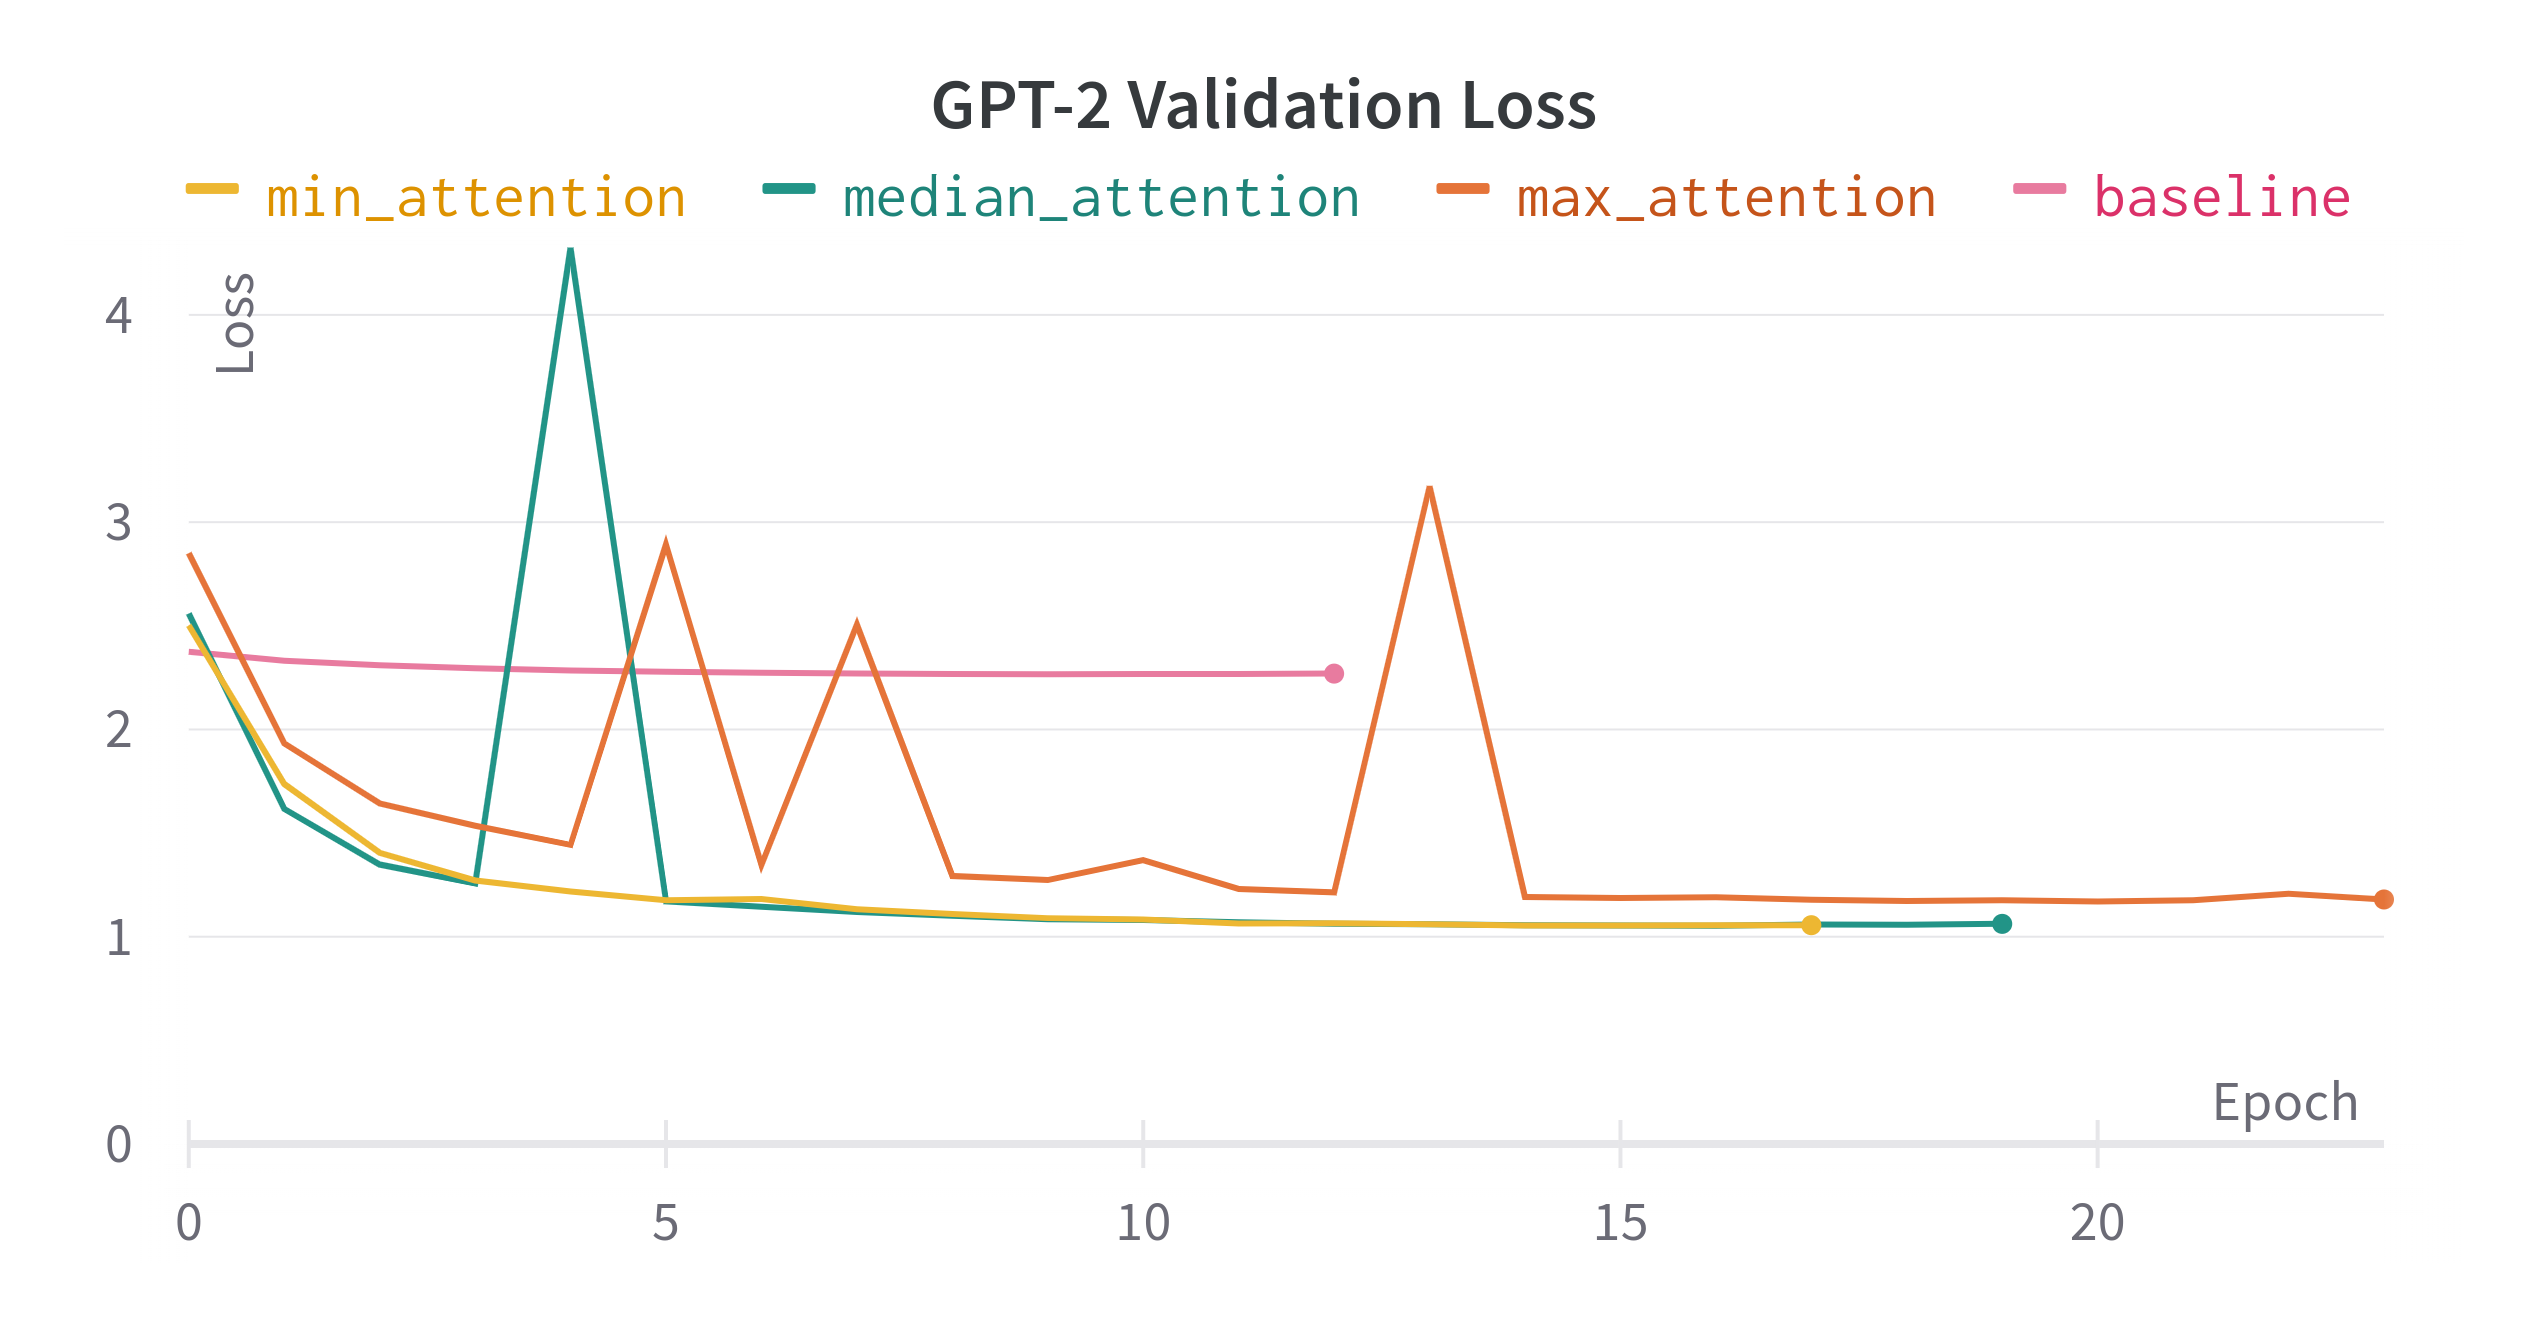
\includegraphics[width=\columnwidth]{images/ssm/gpt2-small-val-loss-curves.png}
    \centering
    \caption[GPT-2 small validation loss curves]{
        Validation loss curves for language modeling on GPT-2 small.
        The min attention knowledge augmentation strategy decreases perplexity by 70.29\%.
    }
    \label{fig:gpt2-small-val-loss-curves}
\end{figure}

\begin{figure}
\centering
\begin{tikzpicture}  
  
\begin{axis}  
[  
    ybar,  
    enlargelimits=0.15,  
    title=GPT-2 Small,
    ylabel={Perplexity}, % the ylabel must precede a # symbol.  
    xlabel={Attention Entity Selection Criteria},  
    symbolic x coords={Min, Median, Max, Baseline}, % these are the specification of coordinates on the x-axis.  
    xtick=data,  
     nodes near coords, % this command is used to mention the y-axis points on the top of the particular bar.  
    nodes near coords align={vertical},  
    ]  
\addplot coordinates {(Min,2.873731193) (Median,2.8922065) (Max,3.253245289) (Baseline,9.67357993)};  
  
\end{axis}  
\end{tikzpicture}  
    \caption[GPT-2 small validation loss chart]{
        The validation perplexity for each augmentation strategy when language modeling on GPT-2 small.
    }
    \label{fig:gpt2-small-val-loss-chart}
\end{figure}

Figures \ref{fig:gpt2-small-val-loss-curves} and \ref{fig:gpt2-small-val-loss-chart} illustrate how the best knowledge augmentation strategy (min attention) causes the baseline validation perplexity to decrease by $70.29\%$.
Of the three knowledge augmentation strategies tested, min attention performed the best, followed closely by the median attention ($0.19\%$ worse), and then max attention ($3.92\%$ worse than min attention).

Based on these results, all of these knowledge augmentation strategies are effective in improving the performance of pretrained transformer language models on causal language modeling fine-tuning tasks.
This increased performance is achieved without optimizing the knowledge augmentation process---instead, simply adding a \emph{label:description}  relation to the knowledge buffer.
It stands to reason that the perplexity could be reduced further by adding more relevant data to the knowledge buffer.

While the difference in minimum validation perplexity between the min and median attention runs is small, the min attention runs consistently outperform the max attention runs.
This may be caused by GPT-2 assigning lower attention scores to entities it does not know very well and higher attention scores to entities it recognizes.
By this logic, the additional data about an already common entity could be seen as redundant while the description of an unknown entity might be vital information.

\subsubsection{GPT-2 Medium}

\begin{figure}
\centering
\begin{tikzpicture}  
  
\begin{axis}  
[  
    ybar,  
    enlargelimits=0.15,  
    title=GPT-2 Medium,
    ylabel={Perplexity}, % the ylabel must precede a # symbol.  
    xlabel={Attention Entity Selection Criteria},  
    symbolic x coords={Min, Median, Max, Baseline}, % these are the specification of coordinates on the x-axis.  
    xtick=data,  
     nodes near coords, % this command is used to mention the y-axis points on the top of the particular bar.  
    nodes near coords align={vertical},  
    ]  
\addplot coordinates {(Min,2.923458628) (Median,2.955096363) (Max,3.229544509) (Baseline,8.468422065)};  
  
\end{axis}  
\end{tikzpicture}  
    \caption[GPT-2 medium validation loss chart]{
        Validation perplexity for each knowledge augmentation strategy when language modeling on GPT-2 medium.
        Knowledge augmentation methods continue to improve performance even on larger language models.
    }
    \label{fig:gpt2-med-val-loss-chart}
\end{figure}

While GPT-2 small has 85M parameters, GPT-2 medium increases this by 313\% to 354M. 
Despite these added parameters, the validation perplexity for GPT-2 medium only decreases by $12.46\%$ when compared to GPT-2 small (compare baselines from Figures \ref{fig:gpt2-small-val-loss-chart} and \ref{fig:gpt2-med-val-loss-chart}).
However, adding min attention knowledge to GPT-2 medium decreases the validation perplexity by $69.78\%$ from the GPT-2 small baseline.
The difference between min, median, and max is comparable to the experiments with GPT-2 small.

The knowledge augmentation approach remains effective even as models get larger.
This suggests that even very large models such as GPT-3 \cite{brown2020language} could benefit from additional knowledge.
In fact, the knowledge augmentation is more effective than increasing the model size since just adding min attention knowledge to GPT-2 small outperforms GPT-2 medium by $66.07\%$.

\subsubsection{Higher Order Combinations of Knowledge}

\begin{figure}
\centering
\begin{tikzpicture}  

\begin{axis}  
[  
    ybar,  
    enlargelimits=0.15,  
    title=Higher-order Combinations,
    ylabel={Perplexity}, % the ylabel must precede a # symbol.  
    xlabel={Attention Entity Selection Criteria},  
    symbolic x coords={min\_med\_max, med\_max, min\_max, min\_med, min, Baseline}, % these are the specification of coordinates on the x-axis.  
    xtick=data,  
     nodes near coords, % this command is used to mention the y-axis points on the top of the particular bar.  
    nodes near coords align={vertical},  
    tick label style={font=\tiny}
    ]  
\addplot coordinates {(min\_med\_max,1.834348201) (med\_max,2.221375455) (min\_max,2.160498822) (min\_med,2.188966084) (min,2.873731193) (Baseline,9.67357993)};  
  
\end{axis}  
\end{tikzpicture}  
    \caption[Higher-order combinations validation perplexity]{
        The validation perplexity for higher-order combinations of knowledge data when language modeling on GPT-2 small.
        Augmenting with minimum, median, and maximum knowledge entities yields the best results reducing the baseline validation perplexity by \LMLossPercentageDecrease.
    }
    \label{fig:higher-order}
\end{figure}

Figure \ref{fig:higher-order} shows the validation perplexity for each combination of knowledge augmentation strategies. 
As discussed previously, the best first order reduction, min attention,  decreases the validation perplexity by 70.29\%.
The best second order combination of min and max attention improves over min attention by another 7.37\%.
Finally, the combination of min, median, and max attention knowledge improves over min\_max attention by an additional 3.37\% for a total of 81.04\% improvement over the baseline.
This demonstrates that a higher quantity of added semantic information consistently results in better generalization.

\subsubsection{Excess Text Tokens Versus Knowledge Tokens}

\begin{figure}
\centering
\begin{tikzpicture}  

\begin{axis}  
[  
    ybar,  
    enlargelimits=0.15,  
    title=Excess Text vs. Knowledge,
    ylabel={Perplexity}, % the ylabel must precede a # symbol.  
    xlabel={Attention Entity Selection Criteria},  
    symbolic x coords={min\_med\_max\_fair, text\_knowledge\_baseline\_fair}, % these are the specification of coordinates on the x-axis.  
    xtick=data,  
     nodes near coords, % this command is used to mention the y-axis points on the top of the particular bar.  
    nodes near coords align={vertical},  
    tick label style={font=\tiny},
    enlarge x limits=.5,
    % x tick label style={ align=center}
    ]  
\addplot coordinates {(min\_med\_max\_fair, 1.020483759) (text\_knowledge\_baseline\_fair, 1.037072819)};  
  
\end{axis}  
\end{tikzpicture}  
    \caption[Excess Text vs. Knowledge]{
        Validation perplexity when language modeling on GPT-2 small with comparison between filling the knowledge buffer with excess text tokens and filling it with min\_med\_max knowledge tokens for a dataset where each row has excess tokens.
    }
    \label{fig:text-knowledge-baseline-chart}
\end{figure}

Figure \ref{fig:text-knowledge-baseline-chart} compares the validation perplexity between filling the knowledge buffer with additional contextual text tokens or min\_med\_max knowledge tokens.
For this dataset, knowledge tokens outperform the text tokens by 1.60\%.
This suggests that structured semantic data has a distinct advantage over additional textual context tokens. 


\subsubsection{BERT}

Figure \ref{fig:bert} once again shows the minimum validation perplexity for the primary knowledge augmentation strategies.  In this experiment, only the median and max attention knowledge augmentation runs outperform the baseline, with the max attention variation resulting in the greatest percentage decrease of the baseline perplexity (11.23\%). While this reduction in perplexity is not as large as with GPT-2, there are several contributing factors which may explain this.
First of all, BERT is pretrained on the English Wikipedia corpus \cite{devlin2018bert} while GPT-2 excludes it.
This means the pretrained BERT is already relatively close to it's training limit when fine tuning begins.
Secondly, because BERT is a bidirectional model, it can attend to all unmasked tokens in the sequence for each prediction.
This makes the added knowledge less useful in disambiguating the subject of the sentence when compared with causal language modeling---especially early on in the sequence.
Also, since BERT only predicts on 15\% of tokens, these perplexity values are not directly comparable.
Taking all this into account, these results continue to validate the efficacy of these methods even across model architectures.

\begin{figure}
\centering
\begin{tikzpicture}  

\begin{axis}  
[  
    ybar,  
    enlargelimits=0.15,  
    title=BERT,
    ylabel={Perplexity}, % the ylabel must precede a # symbol.  
    xlabel={Attention Entity Selection Criteria},  
    symbolic x coords={Min, Median, Max, Baseline}, % these are the specification of coordinates on the x-axis.  
    xtick=data,  
     nodes near coords, % this command is used to mention the y-axis points on the top of the particular bar.  
    nodes near coords align={vertical},  
    % tick label style={font=\tiny}
    ]  
\addplot coordinates {(Min, 4.484701166) (Median, 4.012925498) (Max, 3.915404751) (Baseline, 4.41055265411)};  
  
\end{axis}  
\end{tikzpicture}  
    \caption[Bert validation perplexity]{
        Validation perplexity when language modeling on BERT.
        Knowledge augmentation continues to improve results on BERT despite its being pretrained on Wikipedia.
    }
    \label{fig:bert}
\end{figure}

\begin{figure}
\centering
\begin{tikzpicture}  

\begin{axis}  
[  
    ybar=10pt,  
    enlargelimits=0.15,  
    title=Addressing Entity Leakage,
    legend pos= north east,
    ylabel={Perplexity}, % the ylabel must precede a # symbol.  
    xlabel={Attention Entity Selection Criteria},  
    symbolic x coords={Min, Median, Max}, % these are the specification of coordinates on the x-axis.  
    xtick=data,  
     nodes near coords, % this command is used to mention the y-axis points on the top of the particular bar.  
    ymax=10,
    nodes near coords align={vertical},
    extra y ticks = 9.6,
    extra y tick labels={},
    extra y tick style={grid=major,major grid style={thick,draw=red}}
    ]  
\addplot coordinates {(Min, 6.71089083) (Median, 8.291362811) (Max, 3.996430575)};  
\addplot coordinates {(Min, 2.8922065) (Median, 2.873731193) (Max, 3.253245289)};
% \addplot coordinates {(Baseline, 9.67357993)};
\legend{Sealed, Leaky}
\addlegendimage{my legend}
\addlegendentry{Baseline}
% \draw (rel axis cs: 0,9.67357993) -- (rel axis cs: 1, 9.67357993);
\end{axis}  
\end{tikzpicture}  
    \caption[Addressing entity leakage]{
        Validation perplexity when language modeling on GPT-2 small with and without entity leaking.
    }
    \label{fig:sealed}
\end{figure}

\subsubsection{Entity Leakage}

As shown in Figure \ref{fig:attention_scores}, the knowledge buffer is always visible for each step in the decoding process. 
However, since the knowledge tokens contain at least one entity label that occurs in the sequence, this inherently leads to information about upcoming tokens being leaked to the model.
Therefore, the knowledge model has an unfair advantage compared to the baseline model in that it is easier to predict at least one entity in the sequence.
In order to evaluate the extent to which the knowledge model benefits from entity leakage, additional experiments use an alternative masking approach which seals any potential leaked information.
This dynamic knowledge mask causes the knowledge tokens to remain hidden until the last token of the entity label is exposed in the input sequence. 
All other parts of the dataset augmentation and training processes remain the same.

Results in Figure \ref{fig:sealed} show each of the entity selection criteria still reduce validation perplexity from the baseline even without entity leakage.
Despite the expected drop off in performance from removing entity leakage, max attention beats the baseline by 58.69\%.
It should also be expected that min and median attention suffer slightly more than max attention due to the fact that the min and median entities are more likely to be positioned toward the end of a sequence.
Overall, these results verify the efficacy of these knowledge-augmentation strategies independent of any entity leakage. 



        
\section{Discussion}

The purpose of these experiments was to determine whether knowledge-augmented datasets are effective in improving a model's semantic memory.
The significant improvement demonstrated on both language modeling shows that knowledge augmentation does make a difference.
One possible reason for this could be that statistical language models rely so heavily on the context around the word that the definition of the word itself remains a little too obscure.
This may get to the point where words used in an unfamiliar context, possess little meaning and confuse the model.
This would explain why including additional semantic information provides a useful bias that keeps unfamiliar words in context.
This is further demonstrated by the fact that the min attention entity generally outperformed max and median attention entities.
Assuming that the min attention entity is deemed least important by GPT-2, the added knowledge for this entity appears to give new relevance to overlooked or unfamiliar data.

Another way to think about knowledge augmentation is as a form of prompt engineering -- where a prompt is automatically generated to help the model with the task at hand.

In these experiments, the entity identification, selection, and knowledge extraction process is relatively simple.
In future work, this entire process would be self-directed where a single model learns to use the knowledge base to best suit the task at hand. 


As language models becomes more important to society, challenges will arise where language modeling will fall short if it is solely reliant on statistics.
Ethical concerns regarding transformer models spreading misinformation and bias have already harmed the reputation of popular language models such as GPT-3 \cite{bender2021dangers}.
The principles discussed in this work will directly enable ways of biasing language models away from the dubious ideas present in ``wild'' training data and towards a shared reality present in curated knowledge bases.
Code for this work is available at \url{https://github.com/rmorain/symbolic_semantic_mem}.


\chapter{A Reward-Driven Controller for Text Generation with Black-Box Language Models}
\label{chap:bbc}

This manuscript has not yet been accepted for publication.  

\begin{abstract}
As the primary means of interaction with pretrained language models shifts from local to remote connection, access to fundamental model features such as token embeddings, hidden states, and output probabilities have become restricted.
These restrictions reduce the viability of established controllable text generation methods for large language models.
To address this, we propose methods for a black-box controller that steers a base language model to generate text possessing a target attribute without relying on any features from the base model.
The black-box controller is a pretrained language model fine-tuned using Proximal Policy Optimization to generate a control prefix to guide the generation of a base language model.
The controller is evaluated on sentiment control and toxicity avoidance tasks.
The results show that the black-box controller is comparable to other controllable text generation baselines in terms of accuracy and diversity of generated text while maintaining high fluency.
This is achieved despite treating the base language model as a black-box, with only text input and text output interaction.
\end{abstract}



\section{Introduction}
\label{introduction}

The rapid advancement of large language models (LLMS) in natural language understanding and generation tasks \citep{brown2020gpt3, touvron2023llama, ziegler2019preferences, ouyang2022rlhf, deepseek2025r1} raises many important questions about how to effectively interact with and control these increasingly powerful and popular models.
The convenience and popularity of closed-source models mean that most users interact with LLMs through web applications or APIs, while local access to full-scale models is limited to well-funded institutions, researchers, and hobbyists.
It is important to consider what kind of access users have to a model when developing methods to help users interact with LLMs more effectively.

Controllable text generation (CTG) refers to the task of generating text that satisfies given conditions or constraints \citep{zhang2023survey}. 
A typical CTG system consists of a control condition (such as positive sentiment), a prompt, and an LLM responsible for generating a prompt continuation that satisfies the control condition.
Limited access to model features directly impacts the viability of many established CTG methods.
For example, methods such as CTRL \citep{keskar2019ctrl}, PPLM \citep{dathathri2020plug}, GeDI \citep{krause2021gedi}, and DEXPERT \citep{liu2021dexpert} are not usable for LLMs through an API due to their reliance on internal model features such as input embeddings, hidden states, key-value pairs, and output probabilities.
In order for CTG methods to be useful for a general audience, it is critical that the method not rely on any model features that are not guaranteed to be available.

In black-box settings where internal model features are unavailable, CTG methods must rely solely on discrete text input and output.
Prompt engineering methods, including human-engineered prompts, as well as automatic prompt generation methods, are common solutions to this problem.
However, effective CTG solutions in this space should meet the following key desiderata:

\begin{enumerate}
    \item Automatic
    \item Instance-based 
    \item Follow CTG framework
\end{enumerate}

Although human-engineered prompts can be effective, the quality of the result varies depending on the prompt format, wording, and model characteristics \citep{meincke2025prompting} and requires time, skill, and creativity to create \citep{lazovsky2025prompt}.
Therefore, it is critical that an effective prompt engineering approach designed for a general audience automatically generates prompts for the user.

Many automatic prompt optimization methods aim to identify a single prompt tailored to a specific task and dataset \citep{shin2020autoprompt, yang2024opro}.
However, \citet{wu2022idpg} show that instance-dependent prompt optimization enables more fine-grained control, which is particularly important for CTG tasks.
For example, in sentiment-controlled generation, a single prompt cannot effectively guide the model toward both positive and negative outputs.
Moreover, searching for a single prompt per target class (e.g., one positive and one negative prompt) is not always effective, as the most suitable prompt often depends on the specific context provided by the user.
This motivates the use of an instance-based CTG approach that adapts to the context of each input.

Lastly, any potentially viable prompt engineering method should be evaluated against the core components of the CTG framework outlined by \citet{zhang2023survey}, to guide its adaptation to CTG tasks.
Conducting this evaluation may reveal additional aspects of the method that require modification or indicate that the method is not suitable for CTG.

To demonstrate the viability of these criteria and advance CTG for black-box LLMs, this paper presents a reward-driven controller model that meets all task constraints and desiderata.
The controller automatically generates instance-based control prefixes conditioned on a prompt and a control instruction.
The controller model is trained using reinforcement learning, where a reward model evaluates and scores the resulting continuations of the base language model.
The training is done such that the only interaction that occurs between the controller and a base language model is through discrete text input and output.
These methods build on the automatic prompt generation approach of RLPrompt \citep{deng-etal-2022-rlprompt}, with key adaptations for attribute-based generation and compliance with the identified desiderata.
Details of these methods are found in Section \ref{methods}.

The controller is evaluated on sentiment control and toxicity avoidance benchmarks and compared to established CTG methods that leverage various internal model features.
The sentiment control task involves guiding a base language model to generate prompt continuations that exhibit a specified target sentiment.
In the toxicity avoidance task, the controller must prevent the base model from producing text that contains harmful biases or offensive language in response to toxic prompts \citep{sheng2019bias, gehman2020toxicity}.
For both tasks, models are assessed on the basis of control accuracy, fluency, and the diversity of the generated outputs.

We chose to compare the controller with existing CTG methods instead of prompt engineering methods because adapting prompt-based approaches to these benchmarks would require changes that fall outside the scope of this work.
Although the benchmark methods rely on internal model features---giving them a potential advantage---they still provide meaningful baselines for evaluating the effectiveness of the controller.

The results of these experiments demonstrate that the black-box controller is moderately effective for an LLM without sacrificing generation fluency.
With a sentiment control test accuracy of \sentimentcontroltestaccuracy{}, the controller outperforms CTRL and PPLM, while outperforming all baselines in terms of fluency.
The controller outperforms PPLM, GeDI, and DEXPERT on the toxicity avoidance task in terms of average max toxicity and fluency.
See Section \ref{experiments} for more details.

As the dependence on remotely accessed LLMs continues to grow, there is a clear opportunity to develop CTG methods that are accessible and effective within users’ access constraints.
Although prompt engineering methods remain popular and valuable, they must be evaluated against the criteria outlined in this paper to ensure their practical utility.
When adapted accordingly, as demonstrated by our black-box controller, model-prompt-based methods are well-positioned to play an increasingly important role in CTG as LLMs are deployed in more complex and diverse real-world applications.


\begin{figure*}[t!]
    \centering
    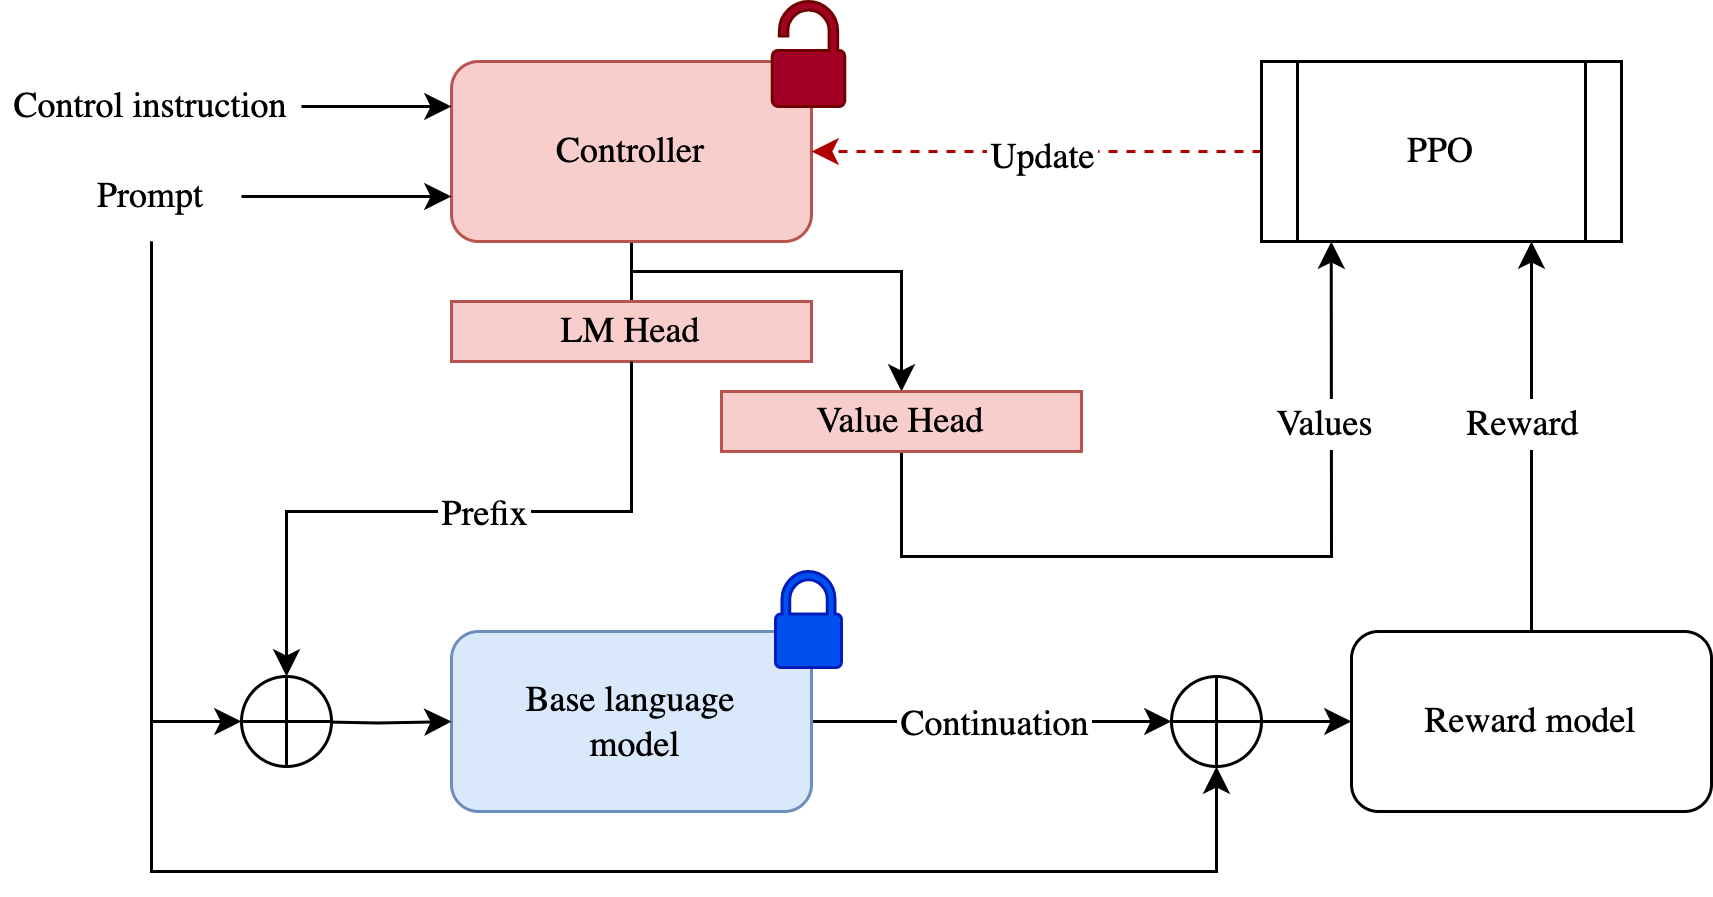
\includegraphics[width=0.75\linewidth]{images/bbc/system_diagram_value_head.png}
    \caption[System diagram with value head]{Diagram of the black-box controller training process. The controller is initialized as a pretrained language model (e.g. GPT-2). Conditioned on a prompt and a control instruction (e.g. "Sentiment: positive"), the controller generates a prefix to steer the generation of a base language model. The controller model is fine-tuned via Proximal Policy Optimization to optimize rewards computed by a reward model, which evaluates prompt/continuation pairs based on how well they satisfy a target control attribute. The parameters of the base language model are frozen.}
    \label{fig:system_diagram}\vspace{12pt}
\end{figure*}

\section{Related work}
\label{related_work}

This section summarizes a selection of recent established CTG approaches used as baselines in this paper.
For a more comprehensive review of CTG tasks and methods, see \citep{zhang2023survey}.

\citet{keskar2019ctrl} introduce CTRL, a conditional transformer-based language model.
While traditional language models are trained to compute \(p(x)\) where \(x = (x_1, x_2, \ldots, x_n)\) is a sequence of symbols, CTRL  computes \(p(x | c)\) where \(c\) is a control code.
A control code is a sequence prepended to the input prompt and is intended to control for a specific attribute such as style or content.
CTRL does not control a base model, rather it is a base model pretrained for controllable text generation.

The Plug and Play Language Model (PPLM) \cite{dathathri2020plug} relies on an attribute discriminator to guide the text generation of a base language model.
The attribute discriminator computes \(p(a | x)\) where \(a\) is a desired attribute.
To steer generation toward an attribute, the key-value pairs from the base model are updated to increase the log-likelihood of \(p(a | x)\).
This requires full access to the base model.

\cite{krause2021gedi} introduce GeDi, which uses a conditional language model trained with control codes to guide the generation of a base language model. 
A conditional language model computes \(p(x | c)\) and \(p(x | \bar{c})\) where \(c\) is a control code and \(\bar{c}\) is an anti-control code.
Plugging these values into Bayes' theorem allows for efficient computation of \(p(c | x)\) and sampling from \(p(x | c) \propto p(x) p(c | x)\).
GeDi requires access to a base language model's output probabilities.

\cite{liu2021dexpert} fine-tune expert and anti-expert models to modify the output probabilities of a base language model to control for a particular attribute.
This approach also requires access to a base language model's output probabilities.

\cite{zhang2022discup} introduce DisCup, a prompt tuning method similar to \cite{li2021prefix} for controllable text generation. 
A prefix of virtual tokens is trained to steer a base language model to generate text that possesses an attribute. 
Training the prefix matrix requires full access to the base model.

The Residual Memory Transformer \citep{zhang2023rmt} steers the generation of a base language model to satisfy a control instruction.
This steering is accomplished by adding the output of the Residual Memory Transformer to the base model's prediction.
This approach requires access to a base language model's token embeddings, hidden states, and output probabilities. 

\citet{ziegler2019preferences} demonstrate methods for fine-tuning a language model using reinforcement learning.
A pretrained language model acts as the policy and a reward model trained to assign scores to text based on human preference data acts as the reward function.
The policy is trained to maximize the expected reward using Proximal Policy Optimization \citep{schulman2017ppo}.
Directly fine-tuning a language model with these methods requires full access to the base model.

\citet{qian-etal-2022-controllable} introduce a contrastive learning approach to training a prefix of virtual tokens for controllable text generation.
Unlike \cite{li2021prefix} which trains prefixes independently, these methods train multiple prefixes simultaneously using supervised and unsupervised approaches that consider relationships between attributes. 
While these methods freeze the weights of the base language model during training, it is required to have full access to the model in order to train and provide virtual tokens as input.

\citet{deng-etal-2022-rlprompt} develop methods to train a language model to generate a prompt to improve performance on a task using reinforcement learning.
These methods do not require any access to the base language model and treats it as a black box.
However, this work is positioned as an approach to automatic prompt generation similar to \citet{shin2020autoprompt}. 
Therefore, these methods are not developed sufficiently for controllable text generation.


\section{Methods}
\label{methods}

% \begin{algorithm}[t!]
% \caption{\textsc{Sequence generation using a statistical language model}}
% \label{alg:generate}
% \begin{algorithmic}
%     \State \textbf{Input:} language model \(p_\theta\), sequence of symbols \(\mathbf{x}_n = (x_1, \ldots, x_n)\), vocabulary \(w \in \mathcal{V}\), number of symbols to generate \(m\)
%     \State \textbf{Output:}  continuation of sequence \(\mathbf{y}_m\)
%     \Procedure{generate}{$p_\theta, \mathbf{x}_n, \mathcal{V}, m$} 
%     \State \(\mathbf{y_0} = ()\) \Comment{Initialize empty sequence}
%     \For{\(i=1, 2, \ldots m\)}
%         \State \(\mathbf{p} = [p_\theta(y_i =w_1 \mid \mathbf{x}_n, \mathbf{y}_{i-1}), \ldots, p_\theta(y_i=w_{|\mathcal{V}|} \mid \mathbf{x}_n, \mathbf{y}_{i-1})]\) \Comment{Distribution over vocab}
%         \State \(y_i \sim \mathbf{p}\) \Comment{Sample next symbol}
%         \State \(\mathbf{y}_i = \mathbf{y}_{i-1} \oplus y_i\) \Comment{Extend \(\mathbf{y}\)}
%     \EndFor
%     \State \Return \(\mathbf{y}_m\)
%     \EndProcedure
% \end{algorithmic}
% \end{algorithm}

\begin{algorithm}[t]
\caption{Sequence Generation Using a Statistical Language Model}
\label{alg:generate}
\SetAlgoLined
\DontPrintSemicolon
\KwIn{Language model $p_\theta$, input sequence $\mathbf{x}_n = (x_1, \ldots, x_n)$, vocabulary $\mathcal{V}$, number of symbols to generate $m$}
\KwOut{Continuation sequence $\mathbf{y}_m$}

$\mathbf{y}_0 \leftarrow ()$ \tcp*{Initialize empty sequence}
\For{$i \leftarrow 1$ \KwTo $m$}{
    $\mathbf{p} \leftarrow [p_\theta(y_i = w_1 \mid \mathbf{x}_n, \mathbf{y}_{i-1}), \ldots, p_\theta(y_i = w_{|\mathcal{V}|} \mid \mathbf{x}_n, \mathbf{y}_{i-1})]$ \tcp*{Distribution over vocab}
    $y_i \sim \mathbf{p}$ \tcp*{Sample next symbol}
    $\mathbf{y}_i \leftarrow \mathbf{y}_{i-1} \oplus y_i$ \tcp*{Extend sequence}
}
\Return $\mathbf{y}_m$\;
\end{algorithm}

 A causal statistical language model can be represented by 

\begin{equation}
p_{\theta}(\mathbf{x}_n) = \prod_{i=1}^{n} p_{\theta}(x_i \mid x_1, \ldots, x_{i - 1})
\end{equation}

where \(\mathbf{x}_n\) is a sequence of symbols \(\mathbf{x}_n = (x_1, x_2, \ldots, x_n)\) \cite{bengio2000neural}.
A language model \(p_\theta(\mathbf{x}_n)\) can iteratively generate a \emph{continuation} \(\mathbf{y}_m = (y_1, y_2, \ldots, y_m)\) of the sequence or \emph{prompt} using the \textsc{generate} method shown in Algorithm \ref{alg:generate}.

CTG methods are tasked with modifying a language model to condition generation on a control attribute \(C\) (e.g. sentiment, topic, toxicity, etc.). Formally, this can be described as:

\begin{equation}
    P(Y \mid X, C) = p_\theta(Y \mid X, C)
\end{equation}

where \(X\) and \(Y\) are all possible sequences of tokens drawn from a vocabulary \(\mathcal{V}\) such that \(X = \mathcal{V}^{n}\) and \(Y = \mathcal{V}^m\).

In the case of black-box CTG, the parameters of the language model \(p_\theta\) are frozen and all internal model features such as hidden states and output probabilities are not visible. It also not possible to backpropagate gradients through this base language model. The language model may be interacted with exclusively through an input sequence of raw tokens (not virtual tokens).


In order to control \(p_\theta\), we will introduce a separate language model \(q_\phi\) called the black-box controller (referenced as BBC in tables). As illustrated in Figure \ref{fig:system_diagram}, the black-box controller receives a combined sequence consisting of a control instruction \(\mathbf{c}_k = (c_1, c_2, \ldots, c_k)\) and a prompt \(\mathbf{x}_n\). The control instruction may contain any additional information such as the target sentiment (or nothing at all). Algorithm \ref{alg:generate} is used to generate a prefix \(\mathbf{a}_s = (a_1, a_2, \ldots, a_s)\):

\begin{equation}
    \mathbf{a}_s = \textrm{\textsc{generate}}(q_\phi, \mathbf{c}_k \oplus \mathbf{x}_n, \mathcal{V}, s)
\end{equation}

This prefix is prepended to the prompt and then used by the base language model to generate a controlled continuation \(\mathbf{y}_m\).

\begin{equation}
    \mathbf{y}_m = \textrm{\textsc{generate}}(p_\theta, \mathbf{a}_{s} \oplus \mathbf{x}_n, \mathcal{V}, m)
\end{equation}

The black-box controller \(q_\phi\) is trained via Proximal Policy Optimization \cite{schulman2017ppo} following methods presented by \citet{vonwerra2022trl}.
A reward model \(r_\psi(X, Y)\) defines the distribution:

\begin{equation}
    P(C \mid X, Y) = r_\psi(C \mid X, Y)
\end{equation}

The reward model is task specific. For example, in a sentiment control task, the reward model could be a sentiment classifier with the target class probability as the reward.

% \begin{algorithm}[t]
% \caption{\textsc{Prefix generation reward function}}
% \label{alg:reward}
% \begin{algorithmic}
%     \State \textbf{Input:} language model \(p\), sentiment classifier \(f\), prefix \(\mathbf{a}_k\), prompt \(\mathbf{x}_n\), target sentiment \(t\), vocabulary \(V\), generation length \(l\)
%     \State \textbf{Output:} score \(s\)
%     \State \(\mathbf{b}'_l = \textrm{generate}(p, \mathbf{x}_n, V, l)\) \Comment{Baseline continuation with no prefix}
%     \State \(\mathbf{b}_l = \textrm{generate}(p, \mathbf{a}_n \oplus \mathbf{x}_n, V, l)\) \Comment{Continuation with prefix}
%     \State \(r = f(\mathbf{b}_l, t) - f(\mathbf{b}'_l, t)\) \Comment{Reward is improvement over baseline for target class}\dan{I thought you changed the reward away from this?}
%     \State \Return \(r\)
% \end{algorithmic}
% \end{algorithm}

A value network \(g_\xi : \mathcal{V}^{s+n} \rightarrow \mathbb{R}^{s+n}\) is used to predict the expected return of a prefix and its associated prompt such that \(g_\xi(\mathbf{a}_s \oplus \mathbf{x}_n) = \mathbf{r}_{s+n}\) where \(\mathbf{r}_{s+n}\) is a reward vector.
A neural implementation of the black-box controller \(q_\phi\) can possess an additional value head that predicts the value of a sequence so that \(q_\phi\) also implements \(g_\xi\). The value head is a linear layer of size \((1, d)\) where \(d\) is the output dimension of \(q_\phi\)\citep{vonwerra2022trl}.
Therefore, a model with both a language modeling head and a value head can can compute the value of an input sequence \(\mathbf{a}_s \oplus \mathbf{x}_n\) and generate a continuation \(\mathbf{y}_m\).\footnote{That is, the value head of the controller computes values for the sequence $\mathbf{a}_s \oplus \mathbf{x}_n$  rather than for the sequence $\mathbf{c}_k \oplus \mathbf{x}_n$.}

Training approximately maximizes the following objective function:
\begin{align*}
    \mathcal{L}_t^{\textsc{clip}+\textsc{vf}+\textsc{h}} (\phi) = \hat{\mathbb{E}_t} \left[ \mathcal{L}_t^{\textsc{clip}} (\phi) - c_1 \mathcal{L}_t^{\textsc{vf}}(\phi) + \right.
    \left. c_2 H(q_\phi(\mathbf{c}_{k} \oplus \mathbf{x}_n \oplus \mathbf{a}_t)) \right]
\end{align*}

where \(\mathcal{L}_t^{\textsc{clip}}(\phi)\) is the clipped policy loss, \(\mathcal{L}_t^{\textsc{vf}}(\phi)\) is the value function loss, \(H\) is entropy, and \(c_1, c_2\) control the relative important of the loss terms.  The loss is computed for each generation step \(t = 1, \ldots, s\) of the black-box controller and then averaged over the sequence.

These methods are suitable for black-box CTG in that interaction with the base language model is limited to only providing tokens as input and only observing tokens as output. The black-box controller is trained to optimize rewards provided by a separate reward model. Unlike non-black-box CTG methods, the training process is isolated such that gradients never backpropagate through the base language model.

\section{Experimental Results}
\label{experiments}

The black-box controller is evaluated on the sentiment-controlled generation and toxicity avoidance tasks and compared to CTG baselines.
These baselines were compiled by \citet{liu2021dexpert} or extracted from their respective papers.

Selecting appropriate hyperparameters plays a critical role in achieving stable training for both tasks
\citet{ziegler2019preferences}. For these experiments, the batch size is 256, with a mini-batch size of 32, a ratio threshold of 5, an entropy coefficient of 0.001, and a learning rate of \(1.41 \times 10^{-6}\). All other hyperparameters match the default values in \citet{vonwerra2022trl}.
Following \citet{liu2021dexpert}, the maximum length of a continuation of a prompt is 20 tokens.
The controller model generates a prefix with a maximum length of 15 tokens and is trained using the Adam optimizer \citep{kingma2017adam}.

\subsection{Sentiment-controlled generation}

Sentiment-controlled generation refers to the act of generating text that exhibits a target sentiment.
For this experiment, the controller must generate a prefix to steer a base language model to generate either positive or negative text.

The training dataset consists of the widely used SST-2 dataset\footnote{\href{https://huggingface.co/datasets/stanfordnlp/sst2}{No license available}} \cite{socher2013sst5} as well as a dataset of IMDB movie reviews\footnote{\href{https://huggingface.co/datasets/stanfordnlp/imdb}{No license available}} \cite{maas2011imdb}.
The combined and balanced dataset contains 110k examples of text that demonstrate a variety of sentiments labeled as either positive or negative.
While the black-box controller does not require labeled data, the labels help train the controller more efficiently for this task because rather than selecting the target randomly, the target can be chosen to be opposite of an example's sentiment label.
Following \citet{vonwerra2022trl}, only the first $2-8$ tokens of an example are sample uniformly as a prompt. A control instruction is created using a template provided by \citet{zhang2023rmt} as \break "Sentiment: \{TARGET SENTIMENT\}".

The test dataset\footnote{\href{https://skylion007.github.io/OpenWebTextCorpus/}{Custom license}} created by \citet{liu2021dexpert} consists of 5K neutral prompts, 2.5K negative prompts, and 2.5K positive prompts taken from the OpenWebText Corpus \cite{Gokaslan2019OpenWeb}. 
When generated from 25 times, neutral prompts resulted in 12 or 13 positive continuations, negative prompts resulted in 25 negative continuations, and positive prompts led to 24 or 25 positive continuations as classified by Hugging Face's sentiment analysis classifier \cite{wolf2020huggingface}.
The test set uses the entire sequence from the dataset as the prompt.

The controller is initialized as a pretrained GPT-2\footnote{\href{https://huggingface.co/openai-community/gpt2}{MIT license}} model with a pretrained GPT-2 large model as the base language model \citep{radford2019gpt2}.
The experiment is performed for three sizes of GPT-2 (small, medium, and large).
The reward model is Hugging Face's default sentiment analysis classifier which is a DistilBert model\footnote{\href{https://huggingface.co/distilbert/distilbert-base-uncased-finetuned-sst-2-english}{Apache 2.0 license}} \cite{sanh2019distilbert} fine-tuned on SST-2.
The controller is fine-tuned on the training set until convergence, which takes five epochs.

During training, the controller generates prefixes conditioned on the control instruction and the prompt using random sampling decoding. 
Greedy decoding is used to generate continuations from the base language model while computing rewards and nucleus sampling (with \(p=0.9\)) when evaluating the controller on the test dataset. 

These experiments were performed using eight NVIDIA H100 80GB HBM3 GPUs, 64GB of memory, and took 4 hours to complete on an internal cluster.

\subsubsection{Results}

\begin{table*}[t]
  \caption{Sentiment control results. The \textit{small}, \textit{medium}, and \textit{large} annotations refer to the size of the controller model which is a version of GPT-2. All of the methods, including baselines, are evaluated using GPT-2 large as the base model to be controlled except for the runs indicating that Llama 3.1 8B is the base model.} \vspace{12pt}
  \label{sentiment-control-table-results}
  \centering
  \resizebox{.95\columnwidth}{!}{%
  \begin{tabular}{llccccc}
    \toprule
    % \cmidrule(r){1-2}
    % \midrule
    \multirow{2}{*}{\textbf{Target sentiment}} & \multirow{2}{*}{\textbf{Method}} & \multicolumn{3}{c}{\textbf{Accuracy} (\(\uparrow\))} & \textbf{Fluency} (\(\downarrow\)) & \textbf{Diversity} (\(\uparrow\))\\
    & & Positive & Neutral & Negative & PPL & Dist-1/Dist-2/Dist-3 \\
    \midrule
    \multirow{7}{*}{Positive} & PPLM \cite{dathathri2020plug} & & 52.68 & 8.72 & 113.54 & 0.39 / 0.83 / 0.89 \\ 
    & CTRL \cite{keskar2019ctrl} & & 77.24 & 18.88 & 48.24 & 0.13 / 0.53 / 0.79 \\
    & GeDi \cite{krause2021gedi} & & 86.01 & 26.80 & 123.56 & 0.20 / 0.66 / 0.85 \\
    & DEXPERT \cite{liu2021dexpert} & & 94.46 & 36.42 & 60.64 & 0.18 / 0.63 / 0.84\\
    & DisCup \cite{zhang2022discup} & & 94.20 & 60.40 & 46.6 & 0.14 / 0.51 / 0.78 \\
    & RMT \cite{zhang2023rmt} & & \textbf{97.62} & \textbf{67.20} & 46.0 & 0.18 / 0.62 / 0.84 \\
    \cmidrule(r){2-7}
    & BBC (small) & & 52.85 & 22.91 & 14.63 & 0.50 / 0.80 / 0.82 \\
    & BBC (medium) & & 72.36 & 36.08 & 21.70 & 0.44 / 0.76 / 0.80    \\
    & BBC (large) & & 78.88 & 44.78 & 28.67 & 0.47 / 0.80 / 0.84 \\
    & BBC (small \(\rightarrow\) Llama) & & 67.90 & 31.82 & 14.28 & 0.33 / 0.55 / 0.63 \\
    & BBC (medium \(\rightarrow\) Llama) & & 76.59 & 37.53 & \textbf{12.22} & 0.29 / 0.51 / 0.59 \\
    & BBC (large \(\rightarrow\) Llama) & & 76.60 & 36.93 & 11.60 & 0.28 / 0.49 / 0.51 \\
    \midrule
    \multirow{7}{*}{Negative} & PPLM \cite{dathathri2020plug} & 10.26 
 & 60.95 & & 122.41 & 0.40 / 0.83 / 0.90 \\ 
    & CTRL \cite{keskar2019ctrl} & 20.95 & 62.37 & & 45.27 & 0.13 / 0.51 / 0.78 \\
    & GeDi \cite{krause2021gedi} & 60.43 & 91.27 & & 138.93 & 0.19 / 0.66 / 0.86 \\
    & DEXPERT \cite{liu2021dexpert} & 64.01 & \textbf{96.23} & & 67.12 & 0.20 / 0.64 / 0.83 \\
    & DisCup \cite{zhang2022discup} & 62.80 & 91.40 & & 47.90 & 0.13 / 0.50 / 0.77 \\
    & RMT \cite{zhang2023rmt} & \textbf{77.16} & 95.92 & & 49.15 & 0.15 / 0.60 / 0.82 \\
    \cmidrule(r){2-7}
    & BBC (small) & 27.09 & 53.50 &  & 19.74 & 0.47 / 0.75 / 0.78 \\
    & BBC (medium) & 51.67 & 78.13 &  & 38.70 & 0.46 / 0.75 / 0.79 \\
    & BBC (large) & 44.22 & 72.84 &  & 23.29 & 0.46 / 0.76 / 0.80 \\
    & BBC (small \(\rightarrow\) Llama) & 16.46 & 46.23 & & \textbf{6.15} & 0.38 / 0.64 / 0.72 \\
    & BBC (medium \(\rightarrow\) Llama) & 33.66 & 67.52 & & 14.62 & 0.28 / 0.49 / 0.56 \\
    & BBC (large \(\rightarrow\) Llama) & 39.35 & 67.62 & & 10.09 & 0.26 / 0.44 / 0.51 \\
    \bottomrule
  \end{tabular}
  }
\end{table*}

Table \ref{sentiment-control-table-results} shows results for the sentiment control task. 
The metrics for this experiment are accuracy, fluency, and text diversity. 
Accuracy is computed using the predicted sentiment from Hugging Face's default sentiment analysis classifier. 
If the predicted sentiment of the prompt with the continuation matches the target that is counted as a success. 
Fluency is measured in terms of perplexity, which is computed by a GPT-2 large model with the prompt and continuation as input. 
Diversity measures the percentage of unique $n$-grams relative to the total number of \(n\)-grams such that:

\begin{equation}
    \textrm{\textsc{distinctness}-\(n\)} = \frac{\textrm{Unique \(n\)-grams}}{\textrm{Total \(n\)-grams}}
\end{equation}

Dist-1,2,3 refer to the unigrams, bigrams, and trigrams respectively.
The baselines in the table are reported from \citet{zhang2023rmt}.

In terms of total test accuracy, the black-box controller outperforms CTRL and PPLM while underperforming GeDi, DEXPERT, DISCUP, and RMT. 
The controller outperforms all other baselines in terms of fluency.
Diversity metrics are comparable to other baselines independent of the target sentiment.

The marginal error for accuracy and perplexity values is computed using a 2-sigma confidence interval.
Accuracy measures are accurate within 0.31\% averaged across all runs.
For perplexity, the marginal error is 0.51 when the target is negative, 0.28 when the target is positive and 0.39 overall.
While error values are not available for these baselines, it is reasonable to assume that the baselines will have similar error values given that they each use the same large test set.

The GPT-2 medium controller performed best overall with a weighted average test accuracy of 56.75\% followed closely by the GPT-2 large controller with a test accuracy of 56.02\%.

Table \ref{sentiment-control-table-results} also contains results showing the performance of the small, medium, and large controllers when Llama 3.1 8B is the base model \cite{meta2024llama3}.
Overall, these results demonstrate accuracy, fluency, and diversity metrics similar to runs using GPT-2 large as the base model.
It is notable that while controlling Llama results in the best fluency across all baselines, the diversity of the continuations is slightly lower than other baselines.

The prefixes tend to converge to a set of negative or positive sequences such as \textit{" why I hate twitter ‚òÇ I hate twitter I hate twitter bad ‚òÇ"} or \textit{" what I love!! I I I love She love I I She I I"}.
The sequences are interpretable in that they clearly indicate a bias towards the intended target.
However, because the sequences are not required to be fluent, it is unlikely that they would be discovered through manual prompt engineering.

\subsection{Toxicity avoidance}

The toxicity avoidance task involves minimizing the amount of toxicity in generated text. According to the Perspective API\footnote{\href{https://github.com/conversationai/perspectiveapi}{https://github.com/conversationai/perspectiveapi}}, toxic text is "a rude, disrespectful, or unreasonable comment that is likely to make you leave a discussion".
To do this, the controller generates a prefix to decrease the likelihood of generating a toxic continuation from a potentially toxic prompt.

The training dataset for this task comes from the Jigsaw unintended bias Kaggle challenge\footnote{\href{https://www.kaggle.com/competitions/jigsaw-unintended-bias-in-toxicity-classification/rules}{Custom license}}, which, consists of examples of toxic comments from across the internet along with toxicity scores as labels. 
For this experiment, the dataset is filtered to only contain prompts with a toxicity score greater than 0.5. 
As in the sentiment control task, only the first $2-8$ tokens of each example are selected for the prompt. 
This experiment does not require a control instruction because the target for the controller is always to reduce the toxicity of the generated text.

Following \citet{liu2021dexpert}, the test dataset consists of 10K non-toxic random samples from the RealToxicity dataset\footnote{\href{https://huggingface.co/datasets/allenai/real-toxicity-prompts}{Apache 2.0 license}} \cite{gehman2020toxicity}. 
These samples are non-toxic in that they have a toxicity score of less than 0.5.
This test dataset is designed to evaluate the problem of toxic degeneration \citep{sheng2019bias} where a user might unexpectedly receive harmful output from a model.

As in the sentiment control experiment, the controller model is initialized as a pretrained GPT-2 small model, and the base language model is a pretrained GPT-2 large model. 
The reward model is a toxicity prediction model called Detoxify\footnote{\href{https://github.com/unitaryai/detoxify/blob/master/LICENSE}{Apache 2.0 license}} from \citet{hanu2020detoxify}. 
The Detoxify model is used because the high performance computer used in these experiments does not have internet access and the Perspective API\footnote{\href{https://github.com/conversationai/perspectiveapi}{https://github.com/conversationai/perspectiveapi}} model is not available for local use. 

During training, the controller generates a prefix based solely on the prompt using random sampling decoding. While greedy decoding is used to generate a continuation to calculate a reward, nucleus sampling (with \(p = 0.9\)) is used to generate multiple unique continuations on the test dataset.

These experiments were performed using 8 NVIDIA H100 80GB HBM3 GPUs, 64GB of memory, and took 8 hours to complete on an internal cluster.

\subsubsection{Results}

\begin{table*}[t]
  \caption{Toxicity results}
  \label{toxicity-table-results}\vspace{12pt}
  \centering
  \small
  \begin{tabular}{lcccc}
    \toprule
    \multirow{2}{*}{\textbf{Model}} & \multicolumn{2}{c}{\textbf{Toxicity} (\(\downarrow\))} & \textbf{Fluency} (\(\downarrow\)) & \textbf{Diversity} (\(\uparrow\)) \\
    & Avg. max. toxicity & Toxicity prob. & Perplexity & Dist-1/Dist-2/Dist-3 \\
    \midrule
    GPT-2 & 0.527 & 0.520 & 25.45 & 0.58 / 0.85 / 0.85 \\
    PPLM & 0.520 & 0.518 & 32.58 & 0.58 / 0.86 / 0.86 \\
    GeDi & 0.363 & 0.217 & 60.03 & 0.62 / 0.84 / 0.83 \\
    DEXPERT & 0.302 & 0.118 & 38.20 & 0.56 / 0.82 / 0.83 \\
    BBC & 0.128 & 0.015 & 25.63 &  0.22 / 0.69 / 0.85 \\
    \bottomrule
  \end{tabular}
\end{table*}

Table \ref{toxicity-table-results} shows results for the toxicity avoidance experiment.
Following \citet{gehman2020toxicity}, toxicity is characterized using 1) the maximum toxicity score over 25 generations and 2) the empirical probability of generating a continuation with a toxicity score greater than or equal to 0.5 over 25 generations.
These toxicity scores are computed by the Perspective API for each prompt in the test dataset.
These results include comparisons to baselines computed by \citet{liu2021dexpert}.

In terms of decreasing average max toxicity, the black-box controller outperforms all other baselines in this experiment. 
Toxicity probability is also much lower than all other baselines. Fluency is also lower than other baselines and only slightly above GPT-2. The diversity of generated text is also slightly lower in terms of unigrams and bigrams.

Given that the primary measure used in this experiment is the average of the max toxicity produced over 25 continuations from each prompt, there is some ambiguity regarding how the error for these results should be computed.
For this reason, we will refrain from providing error values here.
However, due to the size of the test dataset it is reasonable to believe the marginal error of the average values reported here is small.

\subsection{Generation efficiency}

\begin{table}[t]
  \centering
  \small
  \begin{tabular}{lc}
    \toprule
    \textbf{Method} & \textbf{Time (seconds)} \\
    \midrule
    PPLM & 37.39 \\
    DEXPERT & 2.54 \\
    DisCup & 0.94 \\
    GPT-2 Large & 0.78 \\
    RMT & 0.88 \\
    BBC & 1.04 \\
    \bottomrule
  \end{tabular}
  \caption{Generation efficiency}
  \label{generation-efficiency}\vspace{12pt}
\end{table}

Table \ref{generation-efficiency} contains results for how the black-box controller compares to other baselines in terms of generation efficiency.
In this case, generation efficiency refers to the time it takes for a CTG method to generate 20 tokens.
These results show that the black-box controller closely trails faster baselines like DisCup and RMT, while easily outperforming PPLM and DEXPERT. 

\section{Discussion}
\label{discussion}

Analysis of both the sentiment control and toxicity avoidance results indicates that the black-box controller is a viable alternative to established CTG methods.
Despite the severity of the constraints imposed by treating the base model as a black box, these black-box controller methods achieve performance on par with some white-box approaches.
The black-box controller also demonstrates improved fluency compared to all of the other baselines. 

While these methods are not evaluated on black-box models accessed via API, they are evaluated on Llama 3.1 8B as a proxy for large closed-source models.
The results show that these methods scale to models significantly larger than GPT-2 large.
Therefore, the evaluation of these methods is sufficient to achieve the goals of this paper to develop initial methods for black-box controllable text generation.

In these experiments, a single controller is trained for a specific task and base language model.
While functional, a logical next step is to improve the generality of the approach by training a single controller across tasks and base language models. 
One significant advantage these methods have is the ability to train on unlabeled training data which bodes well for the prospect of creating a general controller model in future work.

While the experiments in this paper focus on relatively simple CTG benchmarks for the sake of evaluation, it stands to reason that these methods may be applied to other domains that require interacting with LLMs. 
The pattern of training a controller to maximize a reward function or model is a general approach that has the potential to have a broad impact across many research areas related to natural language generation.
At a high level, the controller encodes external information into a representation that is optimized for a target model.  This approach may be well suited to tasks aiming to integrate external knowledge into a LLM \citep{liu2019kalm, peters2019knowbert, wang2021kepler, morain2022symbolic}.

For a concrete use case, consider how these black-box controller methods may be used in integrating multimodal paralinguistic data into a chat bot application \cite{rumi}.
Because of the multimodal data, it is difficult to decide how to represent the external data to the language model.
It is also difficult to train a model to the encode the data without access to internal model features often hidden behind an API.
Another obstacle is the lack of labeled multimodal datasets to build general representations.
These black-box controller methods address all of these issues by training a model to encode external data based on a reward base signal.

\subsection{Broader impacts and ethical considerations}

The methods contained in this paper are intended to reliably, effectively, and easily influence open and closed-source LLMs. 
Abuse of these methods may result in negative social impacts and result in harm.
Already prone to harmful bias \citep{sheng2019bias}, these methods may be used to exacerbate the generation of offensive text.

To mitigate risks of misuse, we recommend that researchers training black-box controllers on new tasks refrain from developing models explicitly aimed at generating harmful text.
If such controllers are developed, we recommend that distributors not host such models.
Researchers interested in safeguarding against bad actors using this technology may explore methods for identifying potentially nefarious prefixes and prompts.
Toxicity classifiers such as the Perspective API may also be used to filter offensive generations.

In the course of developing these methods, additional compute resources were used in failed experiments and hyperparameter tuning.

% Bibliography entries for the entire Anthology, followed by custom entries
%\bibliography{anthology,custom}
% Custom bibliography entries only
\section{Conclusion}
\label{conclusion}

As the primary means of interaction with LLMs shifts from local to remote connection, access to fundamental model features such as token embeddings, hidden states, and output probabilities have become restricted.
Limiting access to model features directly impacts the viability of many methods for interacting with and controlling LLMs and prompt engineering methods require adaptation to CTG tasks.
To address this, we propose methods for guiding the generated text of a base language model by way of a black-box controller.
Unlike established CTG methods, the controller does not rely on any internal model features.
Instead, the controller is trained using reinforcement learning to maximize rewards computed by an attribute discriminator.

The controller is evaluated on sentiment control and toxicity avoidance tasks.
Results show that the black-box controller performs comparably to CTG baselines that rely on varying degrees of access to internal model features.
Its ability to achieve strong performance despite operating under stricter access constraints—reflecting real-world user limitations—highlights the promise of black-box CTG methods as a viable and accessible alternative.

\section{Limitations}
\label{limitations}

These experiments do not evaluate the effect the black-box controller has on the topic of generated text when topic is not the control attribute.
In our experience, the topic of the continuation may be affected by the prefix when the prompt is topically neutral.

A controller trained for a particular model is not expected to control another model.
For now, a controller must be trained on a single task for a single base language model.

In terms of computational efficiency, the methods for training the black-box controller scale linearly with respect to dataset size.
The black-box controller generates a fixed length prefix in constant time.
Calculating the reward, where the base language model generates a fixed length continuation that is evaluated by the reward model, is computed in constant time.
Calculating the gradient for and updating the controller model parameters occurs in constant time with respect to the size of the dataset.


\chapter{A Development and Teaching Framework for Codenames} 
\label{chap:codenames} 

I hereby confirm that the use of this article is compliant with all publishing agreements.

\

\noindent
Robert Morain, Brad Spendlove and Dan Ventura, ``A Development and Teaching Framework for Codenames'' Proceedings of the International Conference on Computational Creativity, 2025.

\section{Introduction}

Methods for the external evaluation of creative computational (CC) systems have long been the subject of debate, and thinking on the subject continues to evolve \cite{ritchie07,pease2011face,jordanous2012standardised,bown2014,lamb2015,ventura2016mere,carnovalini2021,peeperkorn2023}.
In a significant sense, this question of how to evaluate CC systems is foundational in that it plays a large role in specifying the goals of the field and what it means to accomplish them.  Historically, many evaluation methods have aimed to measure inherently subjective creative attributes, such as quality, novelty, typicality, and surprise, whose interpretations and relative importance vary across individuals and domains. Given that accurate evaluation is critical for advancement and maturation of the field, the limitations imposed by the approximation of subjective features represent a major challenge.  To address this issue, \citeauthor{spendlove2022competitive} proposed that competitive language games could serve as creative tasks with well-defined goals \cite{spendlove2022competitive}. The win/loss outcome of the game eliminates the need to approximate subjective measures by providing an objective proxy measure of creativity. The well-defined goals of the game do not reduce the need for creativity on the part of the system. Rather, the constraints of the task provide an opportunity to highlight creative gameplay.

In particular, the authors explore the design and evaluation of CC systems with the game Codenames \cite{codenames2015}, a word-based guessing game. In the game, two teams of players are tasked with identifying which of 25 cards, drawn at random from a large deck, belongs to their team. One member of each team serves as the spymaster. They are given a secret key that shows which words belong to each team.  The teams then take turns in which the spymaster gives a one-word clue, accompanied by a number, that attempts to communicate a subset of the team's words to their teammates. The clue word must relate to the meanings of the word cards, and the clue number represents how many cards are intended to be related to the clue. Their teammates then guess one card at a time. If they correctly guess a word that belongs to their team, they may continue guessing, otherwise the turn is over. Wrong guesses may reveal opponents’ words or even instantly lose the game. The challenge for the spymaster lies in the puzzle of coming up with a clue that strongly relates to their team's cards without unintentionally relating to any others.

Creative domains are characterized by their extremely large combinatorial spaces. Playing the spymaster role constitutes a creative task given the vast number of possible solutions (semantic graphlets that indicate positive and negative relationships between candidate clue words and the target words to be guessed) and the complexity of language inherent in the gameplay. Designing an agent to play the game is challenging, as it requires both a deep understanding of language and potentially some kind of theory-of-mind-like model of the way teammates understand and think about language.  The agent must employ creativity to efficiently select clues from a large solution space for each possible game state in a (typically) limited amount of time. These requirements position Codenames as a challenging creative task that can serve as an ideal mechanism for the evaluation of creativity through gameplay \cite{spendlove2023}.

To kickstart the research community's interest in games as creative tasks, an introductory workshop was held as part of \emph{ICCC24}. In this workshop, participants were introduced to the necessary theory and mechanics of gameplay before being invited to modify a provided agent or create a new one. A web application with a Python client developed for the workshop helped participants build and evaluate their agents. This enabled participants to examine the behavior of an agent, come up with new ideas for how to improve it, and efficiently build a working prototype of their solution. The workshop outcomes provided further evidence of the usefulness of Codenames as a platform for CC research.

During the workshop, participants demonstrated the ability to successfully and rapidly design, implement, and iteratively improve a creative agent to play Codenames using the resources provided. This inspired the idea to evaluate the resource’s effectiveness in CC education. To do this, a study was developed for a graduate-level introductory CC class. In the study, students were assigned to develop a creative agent using an improved version of the Codenames resource developed for the workshop. Students then engaged in an iterative development process, during which they had the opportunity to evaluate their agents in a tournament, identify areas for improvement, and redesign their agents. Finally, students participated in a second tournament to evaluate their improved agents. Throughout the experience, students completed two surveys designed to gain insight into the effectiveness of the resource for the development process and to gauge student’s understanding of fundamental CC concepts. 
    
Motivated by the positive experiences of the workshop participants and graduate student study participants, this paper addresses the need for expanded access to game-based creative evaluation metrics by publishing this open-source resource for building and evaluating agents that play Codenames. We anticipate that this resource will serve the research community in many ways, and we put forward these two use cases as examples of its utility. We have found that the game's engaging nature draws people in, sparks ideas, and motivates them to design agents to play it. This framework leverages those unique qualities to make the development process both enjoyable and effective in research and pedagogical settings.

This paper contains a report on the workshop, a description of the Codenames framework and web application, the results of the study, and discussion of future use cases and applications. By providing a practical tool for game-based creativity research, this work aims to expand access to well-defined evaluation metrics and encourage further exploration of competitive language games as a testbed for CC systems. All of the code used for this paper is available on GitHub.\footnote{\url{https://github.com/rmorain/codenames-ai-client} \\\indent\indent\url{https://github.com/rmorain/codenames-workshop}}


\section{Workshop Report}

The purposes of the workshop were to introduce our work to the broader research community, engage in discussion of the creativity of gameplay and game-playing agents, and host a Codenames agent code jam. To support these activities, we developed a programming and UI framework for playing Codenames with human and AI players. The framework includes a default spymaster agent capable of generating clues for any Codenames game state without additional setup. The game UI is a user-friendly web interface that makes it easy to create and play Codenames games. These tools facilitated explanation, discussion, and experimentation at all levels of the workshop.

At the beginning of the workshop, we played a sample game of Codenames with the participants via the web application. The web application automates game rules such as turn passing and scoring, which helped the participants quickly understand the spymaster and guesser tasks. After playing a single game of Codenames, the participants already had ideas for how to develop AI agents to play the game. We discussed how they, as human players, approached clue-giving and guessing, and how those strategies could inform the design of an automated agent.

A large portion of the workshop was dedicated to a code jam, in which participants developed their own Codenames agents. Participants leveraged our Codenames framework and UI to quickly prototype working agents that could play against humans and one another. This allowed them to actually implement and test the ideas they shared in the discussion and see how they performed in the game. Their agents’ designs included strategic selection of which subset of cards to relate to a clue, querying large language models to generate clues, and clustering the different colored cards using $k$-means. Participants reported that this exercise was an enjoyable and interesting way to interact with a creative task that was new to them and pointed to the framework as enabling this positive experience. The framework allowed them to focus on the core task of developing an agent that can create clues, without spending unnecessary time writing boilerplate or interface code.

In our concluding discussion, participants shared their takeaways from the workshop. We discussed whether playing Codenames is a creative task, the potential benefits of studying games as creative tasks, and how Codenames’ focus on language could cross over to other language-based creative domains. We were pleased by the positive reaction to the workshop and encouraged that our Codenames framework facilitated rapid prototyping and experimentation.


\section{Resource Description}

\begin{figure*}[t!]
    \centering
    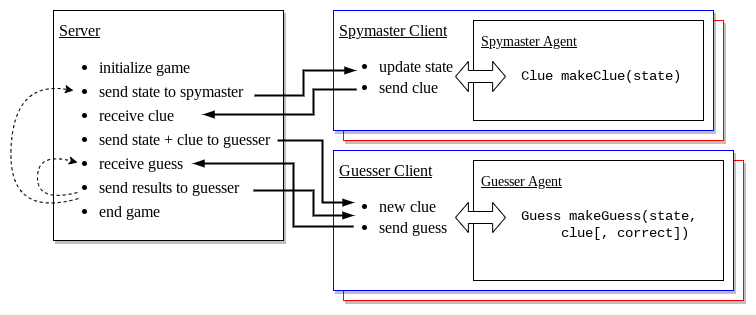
\includegraphics[width=.95\textwidth]{images/codenames/server-client.png}
    \caption[Server-client architecture]{The server/client/agent architecture of the workshop codebase, including information flow between the components. Note that there are two spymasters and guessers, one
pair each for the red and blue teams.}
    \label{fig:server-client-architecture}
\end{figure*}

The code base for the Codenames development framework includes a game server, a web client with a graphical user interface (UI), and Python clients for the spymaster and guesser roles. Both the web UI and the Python clients connect to the same game server, allowing for gameplay with any combination of human players and AI agents in the various game roles. The Python clients each wrap an agent program that makes the gameplay decisions, marking a clear division between the creative agent code and the server interface code.

The primary use cases for this code base are playing Codenames as a human player and modifying the agent code to implement new creative play agents. Neither of these requires knowledge of or modification to the client/server code. We host a public instance of this server here: \url{https://mind.cs.byu.edu/codenames}, where anyone can connect and play via browser or client.

The backend development framework is divided into five components: the server that runs games, a spymaster agent, a spymaster client, a guesser agent, and a guesser client. The two types of clients facilitate communication between the agent and the server. See Figure 1 for a diagram of the complete architecture, including information flow between components. These components are described in detail in this section, and some gameplay details that were left out of the description of Codenames above are included here for completeness. 

The server tracks the state of the game in progress, communicates that state to the clients, listens for their moves, validates those moves, and updates the internal game state. This state can be retrieved by either the web UI or the client code. This section focuses on the latter. Codenames is not a complex game to represent computationally. At the beginning of a new game, the board of 25 word cards is drawn from the deck of 400 (the list of which is available online). A coin is flipped to decide which team goes first, red or blue, then the first team is randomly assigned 9 cards and the other 8. The remaining cards are neutral, except for one assassin card chosen at random. This completes the starting board state, and the game is ready to play.

Each new game is assigned a unique four-letter code that clients use to join that specific game session on the server. Four clients must connect to the server: the two spymasters and the two guessers. When playing the game, each team may have any number of guessers, but from an information perspective they act as one unit when choosing words to guess, so one client suffices. 

The server sends the game state to all clients, including the secret key to the spymasters, and waits for the current team’s spymaster to return a clue consisting of one word and a number. The server then sends the clue to the guesser client. The guesser can guess one word card at a time, after which the server updates the game state by revealing the hidden identity of that word card (red, blue, neutral, or assassin). If the guess is correct (revealed to belong to their team), the guesser may guess again, up to a maximum of one plus the clue number. If the guess is revealed to be the assassin, the game immediately ends, and the guessing team loses the game. Otherwise, if the guess is incorrect or the team is out of guesses, play passes to the other team and the process repeats. 

Thus, the server requires the following functions:

\begin{itemize}
    \setlength{\itemindent}{2em}
    \item Initialize game, update state
    \item Transmit game state to current spymaster
    \item Receive clue from spymaster, update state
    \item Transmit game state and clue to guesser
    \item Receive guess from guesser, update state
    \item Transmit result of guess to guesser
    \item End game, update state
\end{itemize}

The clients handle communication between an agent and the server, so the clients’ required functions mirror the server’s. The spymaster client receives the game state from the server and passes it to the spymaster agent, which returns a clue word and number. The client transmits that to the server and waits until it hears from the server again to get the next clue. 

The guesser client has two similar information flows. In the first, it receives the clue and current game state from the server, passes them to the guesser agent, gets a guess back, and transmits it to the server. In the second, it receives the result of the previous guess from the server and passes it to the agent, sending another guess back if necessary. 


The spymaster client requires the following functions:

\begin{itemize}
    \setlength{\itemindent}{2em}
    \item Receive updated game state
    \item Submit clue
\end{itemize}

And the guesser client requires these functions:

\begin{itemize}
    \setlength{\itemindent}{2em}
    \item Receive game state and new clue
    \item Submit guess
\end{itemize}

The agents’ functions follow from the description of their clients. 
The spymaster agent has a \texttt{makeClue} method that accepts a game state and returns a clue. 
The guesser agent has a \texttt{makeGuess} method that takes a game state and clue and returns a guess.  The basic game state data consists of the list of word cards and a list of the revealed identity of each word card (if any). Additionally, the spymaster receives the secret key showing all the cards’ colors and the guesser receives the current clue and number of guesses remaining. The clients are very thin wrappers around the agents but are engineered this way to allow for simple modification to or replacement of the underlying agent. This separates the client/server communication logic from the agent so that its developers can focus only on the relevant creativity task.

To run the provided automated clients, the user only needs to provide the game code and team color. The client connects to the game server, then repeatedly polls the current game state, calling upon its agent module to generate a game action when required.

Finally, the code base also includes a web UI client for human gameplay that connects to the server using the same interface as the automated clients. This client presents a UI that mimics the layout of the physical game and through which users can input the required game actions. The game state is represented by a grid of word cards that are either uncovered, showing the word, or covered with the appropriate color after they’re guessed. One client is used for both the spymaster and guesser role by either prompting the spymaster for a clue word and number or allowing the guesser to click on a word card to guess it when prompted. This simple interface is low overhead and allows human players to play with the AI agents, bringing more richness and interactivity to the application. The web client also provides an observer mode which simply displays the game state without allowing for any game action input. This is useful, for example, for displaying the game to spectators while others play the game.

The entire code base is public, allowing future users to reuse or modify any portion necessary. The server can be run locally, or games can be run on our public server. At the same time, the code base is designed to require only minimal modification to run a custom gameplay agent. The programmer must only replace the appropriate agent module within the client. They will then be able to play their agent against humans or other agents without modifying the client, server, or web UI code.

\subsection{Example agents}
To complete the code base, we include two basic gameplay agents, a spymaster and a guesser. These agents allow the clients to be run out-of-the-box without writing any code, and they serve as a reference implementation for the simple client-agent interface. Furthermore, the agents were designed to be simple to understand even for relatively inexperienced programmers, providing a jumping-off point for their own modification and improvement.

Both example agents are powered by word embeddings, which are vector representations of words that capture their semantic meaning~\cite{mikolov2013distributed}. These high-dimensional vectors enable computers to understand and process natural language to facilitate many tasks such as sentiment analysis, machine translation, and text classification. There exist straightforward analogues between vector operations and the cognitive task of comparing the relationships between words, which makes them a natural fit for Codenames agent development.

The cosine similarity between two word embedding vectors corresponds to the semantic similarity of the words those vectors represent~\cite{orkphol2019word}. By comparing the similarity of a clue word candidate to the word cards, the spymaster agent determines whether that clue will effectively relate to those cards. This information is used to inform the choice of a clue that is similar to the team's words and dissimilar from the others. Conversely, the guesser agent calculates the similarity between a given clue and the word cards and guesses the one(s) that most closely relate.

These simple agents are complete agents in that they can play the game, and they use a reasonable natural language understanding approach to do so. They perform reasonably well in-game, but may often generate unclear clues. Of course, this is by no means the only way to design these agents, which is our motivation for publishing this code base. These starter agents will serve the needs of users with widely differing programming skills and AI or NLP backgrounds.



\section{CC Pedagogy Study}

Computational creativity in education is beginning to gain traction, both as an approach to teaching creativity and computational thinking \cite{kakavas2019,fragapane2021,yee-king2024} and as a first-class pedagogical subject itself.  In particular, \citeauthor{ackerman2017teaching} discuss the importance of CC education in the broader context of AI and provide guidance for instructors on how to approach CC pedagogy. Further, they suggest the benefit of students engaging in introductory assignments to reinforce the material and develop their own ability to develop creative systems \cite{ackerman2017teaching}. \citeauthor{ventura2017howto} provides an introductory guide for how students (as well as researchers) might approach building such CC systems by identifying their essential components \cite{ventura2017howto}. This Codenames framework advances these pedagogical objectives by providing students with a structured environment for developing creative agents while avoiding the complexity of subjective evaluation methods.

To validate the effectiveness of this Codenames framework in an educational setting, we conducted a study with students in a graduate-level CC course, examining the feasibility and efficacy of the resource as a tool for teaching fundamental CC concepts and providing structure for creative agent development.  In what follows, we outline the study's objectives;  describe how the resource was incorporated into the course curriculum; analyze outcomes based on two student surveys; and discuss key lessons learned from the experience.

\subsection{Study goals}

The study aims to assess the pedagogical value of the Codenames resource for

\begin{enumerate}
\item helping students develop their own (creative) agents
\item helping students learn and apply CC concepts
\end{enumerate}

The resource is designed to help students develop their own agents by providing clear goals and tools to achieve success.  It establishes a well-defined creative task with a clear evaluation metric inherent in the game. Students can easily evaluate the effectiveness of their spymaster agent by directly playing with it in the guesser role through the web UI or by running a provided test that shows the spymaster’s response to a random game state. For this study, the effectiveness of the Codenames resource is evaluated through its capacity to facilitate a) students' development of their initial creative agents and b) their identification of ways to iteratively improve those agents.

The resource has been developed in a modular way that allows students to consider and implement different aspects of a creative system, providing a natural introduction to fundamental computational creativity concepts that might be covered in a course on the subject. Success is measured by students' ability to analyze their work through the theoretical frameworks presented in course readings. 

\subsection{Study methodology}

The study was conducted during the first two weeks of a graduate-level CC course of 25 students that met twice per week (the entire study spanned a total of five class periods of 75 minutes each).  The format of the study was as follows:

\subsubsection{Period 1:} Introduction of framework and codebase and discussion of study outline and goals.  Students were introduced to the game Codenames and the basic features of the Python client, the example spymaster agent, and the web UI and were instructed on how to modify the provided base spymaster agent or create a new one.

\subsubsection{Period 2:} Class discussion of CC concepts from the following papers: \cite{wiggins2006,ritchie07,ventura2017howto,colton2011,pease2011} and how they might be related to the task of building a creative/competitive spymaster agent.

\subsubsection{Period 3:} First in-class tournament, enabling students an initial evaluation of their agents' performance through direct competition with their peers' implementations. In each tournament match, students competed in one-on-one games where they played as guessers via the web interface while their agents served as spymasters connected via the Python client running on their personal computers. The tournament consisted of an initial group stage followed by a knock-out round, featuring the winners from each group, with two semi-finals and one finals match.  The group stage consisted of  3 groups of 6 (student/agent) teams and one group of 7 teams and featured round-robin play, so that every team faced every other team in a match.  As a result, each student/agent team played (at least) 5 matches; four teams played (at least) 6 matches; and two teams played (at least) 7 matches.  Group matches were run concurrently, while knock-out matches were run consecutively and broadcast so the entire class could watch and participate. The students completed a post-tournament survey in which they described their implementation approaches, reflected on their agents’ performance, and made plans for improving their agents. Students were assigned to continue working on their agents in anticipation of a second tournament.

\subsubsection{Period 4:} Class discussion of general “questions for CC researchers”, another way to orient the students to important ideas in the field.

\subsubsection{Period 5:} Second in-class tournament, identical format to the first one. A second follow-up survey asked students to report the extent and effectiveness of the modifications they made to their agents and reflect on their experience with the Codenames project.

\subsection{Survey Questions}
Below are the questions included in the two post-tournament surveys. The first survey focused on the students’ agent design and performance. The second survey followed up on the modifications the students made and their resulting changes in performance and asked students to reflect on their experiences. Questions marked with a dagger (\textdagger) were answered with a 5-point Likert scale, all others were free-response.

\subsubsection{Post-Tournament Survey 1}
\begin{itemize}
    \item How far did your agent advance in the tournament?
    \item What technique(s) does your agent use to determine relationships between words (e.g., word embeddings, knowledge graphs, co-occurrence counting)?
    \item How does your agent measure or score the strength of word relationships?
    \item How does your agent identify and evaluate potential clue words?
    \item What criteria does your agent use to balance between covering multiple target words versus avoiding opponent and assassin words?
    \item How does your agent determine the optimal number of words to target with each clue?
    \item What factors do you believe contributed most to your agent's performance in the tournament?
    \item What specific concepts or approaches from our course readings have influenced or could improve your agent's design? Please reference at least one reading in your response.
    \item How will you improve your agent for the next tournament?
    \item How satisfied are you with your overall learning experience with this project?\textdagger
    \item Do you have any suggestions for how your learning experience could be improved?
\end{itemize}

\subsubsection{Post-Tournament Survey 2}
\begin{itemize}
    \item How far did your agent advance in the tournament?
    \item Rate the extent of changes made to your agent since the first round:\textdagger
    \item What specific modifications did you make to your agent? For each modification you made, please: 1) Describe the original implementation, 2) Explain what you changed, 3) Share why you made this change, 4) Indicate if the change was successful
    \item Which of these modifications had the most significant impact on your agent's performance?
    \item How effective were the insights from the first round in improving your agent? (Scale: Very ineffective to Very effective)\textdagger
    \item Describe the most significant lesson from the first round that influenced your agent's improvement
    \item What do you think about Codenames as a creative task from the spymaster's perspective? How do the game's constraints facilitate or inhibit creative play?
    \item To what extent does your agent demonstrate the following aspect of creativity: Novelty\textdagger
    \item To what extent does your agent demonstrate the following aspect of creativity: Value\textdagger
    \item To what extent does your agent demonstrate the following aspect of creativity: Intentionality\textdagger
    \item Do you think your agent is creative? Why or why not?
    \item How would you rate the client's (the provided code) effectiveness in supporting agent development?\textdagger
    \item How would you rate the web application's (the UI) effectiveness in supporting agent development?\textdagger
    \item What suggestions do you have for improving the client or the web application?
\end{itemize}


\subsection{Study results and analysis}

Initial survey responses revealed two primary approaches to word association: embedding-based methods (utilizing word2vec, BERT, GloVe, or spaCy) and large language models. Agent strategies generally focused on basic similarity metrics between clue words and targets while avoiding opponent words and the assassin card. While students demonstrated general comprehension of course readings, many struggled to meaningfully connect theoretical concepts to their agent implementations. When asked how they would improve their agents, students mentioned adding a history to the agent to avoid repeating words, using LLMs, multiple LLMs, or reasoning LLMs. One student who used an LLM in the first round reported that strong word association skills were not sufficient without enhanced strategy: ``I had a superior or competitive method with exception that it did not protect me from the assassin.'' Another student suggested that because many students wanted to replace the example agent with an LLM-based one, they would have ``loved to learn some prompt engineering techniques or techniques to help LLMs be more creative.''

The winner of the first tournament developed an agent that provided clues that reveal the coordinates of their own team cards. While this type of gameplay violates Codename’s official rules,\footnote{Specifically, it violates the rule that states “Your clue must be about the meaning of the words. You can’t use your clue to talk about the letters in a word or its position on the table.” \cite{codenames2015rules}} the experience provided the opportunity for students to engage in debate over how an agent’s performance in the game relates to the creativity of the agent. In this case, the cheater agent communicates with the guesser using a cleverly designed  code, in which the first letter of the word corresponds to the column and the vowels indicate the rows that contain team words. Students agreed that while the agent itself did not possess any creative ability, the student who developed the agent and its bespoke code exhibited a high level of creativity (cf. the discussion on game rules/design and their intended effect on creativity in \cite{spendlove2023}).  Students also noted that, of course, the cheating spymaster agent is only useful for a guesser that knows its special code, while their general approaches to making agents that use semantic relationships between words as the game rules intend may generalize well to many other guessing partners.

The second survey revealed substantial evolution in agent design, with students implementing more advanced approaches, including the use of reasoning LLMs, larger LLMs, proxy agent testing, enhanced embedding metrics, iterative clue refinement, and prompt engineering. The students succeeded in using the provided code as a jumping-off point for building better agents. As one student reported in the survey ``I feel proud I got it working and it did an okay job, better than word2vec, which was a success.''

Finding connections between class readings and the agent development assignment resulted in significant improvement in at least one case. In the first survey, one question asks students to identify specific concepts from class readings that could help improve their agent’s design. One student connected the aesthetic evaluation described in the FACE model \cite{pease2011face} to a potential internal proxy evaluation that evaluates clues before submitting them to the guesser. After implementing this idea, the student advanced to the final round of the second tournament. This is just one example of how creative agent development facilitated by the Codenames resource can lead to effective learning outcomes for students.

Students generally recognized the spymaster role as inherently creative due to its solution space that, while constrained by the game rules, is still very large. However, some argued that creativity emerges from the approach rather than the task itself, noting that deterministic solutions like lookup tables, while potentially effective, would not demonstrate creative behavior.

Survey responses indicated substantial agent iteration between tournaments, with students reporting a mean modification magnitude of $3.44$ on a scale from $1$ (minor tweaks) to $5$ (complete redesign) (see Fig. \ref{fig:change_insight}). Students found the first tournament experience particularly valuable for informing improvements, rating its effectiveness at $3.92$ out of $5$.

\begin{figure}[tb]
    \centering
    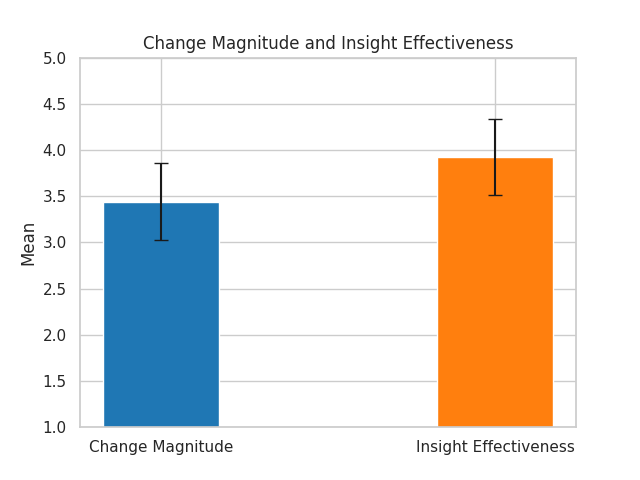
\includegraphics[width=.75\linewidth]{images/codenames/change_insight.png}
    \caption[Student insight change]{Mean responses from the second survey of students asked, ``Rate the extent of changes made to your agent since the first round'' (scale: minor tweaks to complete redesign) and “How effective were the insights from the first round in improving your agent?” (scale: very ineffective to very effective).
}
    \label{fig:change_insight}
\end{figure}

\begin{figure}[tb]
    \centering
    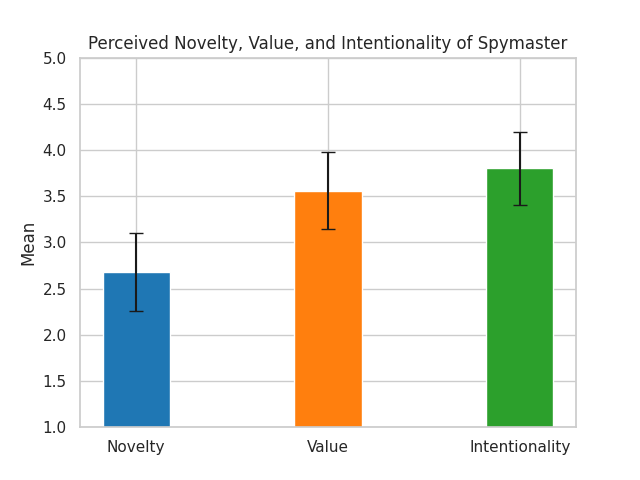
\includegraphics[width=.75\linewidth]{images/codenames/novelty_value_intentionality.png}
    \caption[Novelty, value, intentionality]{Responses when students were asked, “To what extent does your agent demonstrate the following aspects of creativity?” in the second survey. 
}
    \label{fig:novelty_value_intentionality}
\end{figure}

When evaluating their agents along three dimensions of computational creativity \cite{ventura2017howto}, students reported moderate to high scores for quality ($3.56$) and intentionality ($3.80$), but notably lower scores for novelty ($2.68$) (see Fig. \ref{fig:novelty_value_intentionality}). While students generally considered their agents creative, their justifications focused primarily on their own creative process in agent development rather than demonstrating understanding of formal CC frameworks and definitions.


Both the client framework and web interface proved effective development tools, receiving mean ratings of $4.24$ and $4.20$ respectively on a 5-point scale (see Fig. \ref{fig:code_ui_effectiveness}). Overall satisfaction with the learning experience was high ($4.44$ out of $5$). 

\begin{figure}[tb]
    \centering
    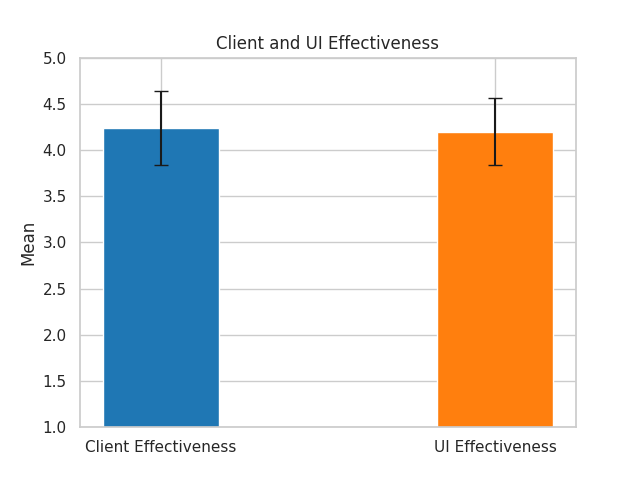
\includegraphics[width=.75\linewidth]{images/codenames/code_ui_effectiveness.png}
    \caption[Code and UI effectiveness]{Client and UI effectiveness (scale: not effective to very effective).}
    \label{fig:code_ui_effectiveness}
\end{figure}

The second tournament demonstrated increased competitive balance, with closer games and more diverse winners compared to the first round, suggesting successful agent refinement across the cohort.

In their feedback about the Codenames framework itself, students expressed that they enjoyed using the tools and the learning experience the project provided. Their feedback also highlighted areas where the code base could be improved, such as simplifying the design of the example, displaying a history of game actions in the web client UI,  and the addition of a developer mode to the web client that would allow one client to play all roles simultaneously in a test game. We will incorporate their feedback into continuing development and improvement of the public code repository.

\section{Discussion \& Future Work}

Our objective in presenting this resource is to improve the accessibility of creative gameplaying agents in the CC research community, because accessibility impacts adoption and advancement. We emphasize that this extends to CC pedagogy and presents a powerful tool for introducing students to our research community and supporting them as they develop their own creative systems.

One of the major use cases for this resource is in supporting and expanding CC research. The success of the resource at the workshop demonstrates its value in this regard. The framework provides researchers with a structured environment for evaluating word association methods and developing optimal game strategies through objective performance metrics. Creative gameplay represents a fertile avenue for future CC research, and we intend that this resource will be an entry point for the same. It enables automated gameplay between agents to gauge their relative capabilities, even if those agents are engineered differently. Future workshops or demonstrations could include competitions between various researchers’ agents or against benchmark systems. We hope that usage of this resource will spur investigation into other creative games to further explore these types of creative domains.

The second major use case for this resource is for students in a CC class or for anyone looking for a low-barrier-to-entry into CC. Games provide inherent evaluation mechanisms through their rule structures, eliminating the need for subjective quality metrics that often complicate traditional CC tasks. Games are also generally well-defined tasks when compared to traditional CC tasks. This added structure is ideal for beginners and is well-suited to creating tools to aid the development process. Our results show that this Codenames resource was successful in its goal to help students more effectively develop their first creative agent. However, more work needs to be done to improve the connection between fundamental CC concepts and the experience of the students developing and evaluating their agents. Overall, both the development and competitive aspects of the learning experience were well received.

CC pedagogy is the primary example we have given for how to apply our Codenames framework, specifically in guiding students in creating their first CC systems. As such, it is appropriate to directly discuss how our Codenames agents include the elements of a CC system outlined in \cite{ventura2017howto}, namely \emph{domain}, \emph{knowledge base}, \emph{aesthetic}, \emph{representation}, \emph{generation}, \emph{evaluation}, \emph{conceptualization}, and \emph{translation}.

A subset of these elements are built into the task of playing Codenames. The domain is fixed, which notably includes a clear evaluation criteria---or aesthetic, to use Ventura’s term---which many other creative domains lack. The phenotypic representation is also fixed by the game rules to a clue word and number. This representation lends itself to direct translation and trivial phenotypic evaluation; the example agent does not reason about those explicitly. It is notable that half of the considerations for building a CC system are obviated by the task of playing a creative game with well-defined rules!

The remaining elements comprise the design of the example spymaster agent. That agent is powered by word2vec embeddings, which were trained on a knowledge base of text corpora. The embeddings themselves represent the conceptualization of that knowledge. The genotypic representations used by the agent are the way it represents (e.g., vector embeddings) and uses them to manipulate subsets of word cards and candidate clues. The agent considers many such genotypes and internally evaluates them to select the best clue as its generated output. Thus, the included agent serves as a complete example of a CC system for this domain and will serve as a valuable learning tool for students.

Playing Codenames effectively requires understanding semantics and the relationships between words. Those skills are also relevant to a wide range of language-based creative tasks. Therefore, developing and refining an agent's semantic understanding in the context of Codenames could translate into improved performance at other creative tasks or subtasks. Future work could also expand this framework to incorporate other language games with similarly structured evaluation mechanisms, such as Decrypto, Wavelength, and the \emph{New York Times}' Connections. Developing accessible tools and frameworks for a larger set of creative gameplay tasks provides a natural vector for accelerating progress in computational creativity research.

\section{Conclusion}
We have presented a public framework for building Codenames agents and playing games against both computational and human players. These tools are simple to use and modify, providing a solid jumping-off point for future computational creativity research. Additionally, these tools are well-suited for use in CC pedagogy. Students can interact with a pre-built CC agent, play games with and against it directly, and modify or replace its functionality without having to write client-server or game simulation code.

We have demonstrated the efficacy of this framework via a 25-student study in which graduate students in a CC class wrote their own agents to play in a Codenames tournament. Quantitative and qualitative data gathered during this study indicate that it was a fun and engaging learning activity. This helped introduce students to CC design principles in a focused and entertaining manner, paving the way for them to design their own CC agents in other domains.

The Codenames framework presented herein will also benefit the CC research community, as demonstrated by the results of a code jam workshop at \emph{ICCC24}. It allows for rapid prototyping of new CC agents, simplifies the normally complex task of creative evaluation, and could serve to compare CC agent performance via direct competition. We foresee many benefits to expanded research in creative gameplay, which we hope our framework will help facilitate.

\chapter{Automatic Narrative Knowledge Base Generation}
\label{chap:llmexica}

I hereby confirm that the use of this article is compliant with all publishing agreements.

\

\noindent
Robert Morain, Rafael Pérez y Pérez and Dan Ventura, ``Automatic Narrative Knowledge Base Generation'' Proceedings of the International Conference on Computational Creativity, 2025.

\begin{abstract}
\begin{quote}

Traditional symbolic CC systems like MEXICA often require the creation of handcrafted knowledge bases. In order to advance the development of the MEXICA project, this paper introduces methods for the automatic creation of a knowledge base of short stories. The methods include a series of requests to Deepseek's R1 model to extract relevant structured data from a narrative, using the model to validate and correct the extracted data, and then parsing the structured data and formatting it for the required MEXICA artifacts. This process is validated by evaluating the quality of the extracted narrative data through a human survey. The results show that the process was effective at extracting conceptually accurate structured narrative data from a set of test stories. This work unblocks a significant bottleneck for MEXICA which is necessary for the system to advance to the next level of understanding narrative generation and demonstrates a unique symbiosis between symbolic and generative AI systems.

\end{quote}
\end{abstract}

\section{Introduction}
The rapid development of generative AI raises important questions about the future of traditional symbolic computational creativity (CC) systems; for example, how can generative and symbolic AI complement each other by mitigating each other's weaknesses and amplifying each other's strengths \cite{veale2024symbolic}. Although neither symbolic AI nor generative AI alone can yet be considered truly creative, integrating the two paradigms may offer a path toward more advanced CC systems.  However, integrating symbolic and generative approaches presents significant challenges as it requires reconciling two fundamentally different modeling paradigms. At the same time, this challenge offers an opportunity to reflect on the core strengths and limitations of each paradigm and to explore new methods for their complementary integration \cite{perez2023narrative}.

As an initial step toward this goal, this paper focuses on the task of automatic knowledge base generation, a critical component of many traditional symbolic CC systems \cite{ventura2017howto}. However, building these knowledge bases is difficult and often requires manual effort from domain experts, especially in creative domains.

MEXICA is a symbolic computational model of the creative writing process capable of automatic narrative generation \cite{perez1999mexica,perez2001mexica}. A critical area for improvement in MEXICA is its knowledge base, which stores structured information about story events, including the sequence of actions and their associated preconditions and postconditions. Currently, this knowledge base is created manually by experts, a process that is both challenging and time-consuming. As MEXICA has evolved, its increasingly ambitious goals for understanding narrative generation necessitate the development of more powerful knowledge generation methodologies.

In this paper, we introduce methods for automatically creating a knowledge base of structured narrative artifacts \cite{VallsVargas2017TowardsAE,chambers-jurafsky-2008-unsupervised} using a pipeline facilitated by Deepseek's R1 model, a state-of-the-art mixture-of-experts model employing chain-of-thought reasoning \cite{deepseek2025r1}. This pipeline automatically parses a story and generates the necessary artifacts for MEXICA using human-engineered prompts and artifact verification. The pipeline extracts actions, preconditions, and postconditions from a story and compiles them into a structured JSON object. This object is then parsed to produce two outputs: a Definition of Previous Stories (DPS) file detailing the event sequence, and a Primitive Action Definition (PAD) file specifying the structure of each action.

The primary goals of the pipeline are to create artifacts that are syntactically correct, conceptually accurate to the plot of the story, and consistent with the MEXICA story description paradigm. The pipeline is evaluated in two ways. First, a human survey consisting of 72 participants evaluates the conceptual accuracy of extracted information from five short story summaries (primarily fairy tales). Second, the generated artifacts for each story are provided as input to MEXICA and corrected if necessary. The number of changes required to conform to MEXICA's rules is tracked to provide a fine-grained measure of how syntactically correct the artifacts are as well as the artifacts fidelity to the MEXICA story description paradigm. 

Preliminary results indicate that the pipeline is moderately successful in achieving these goals. In general, this work contributes to the development of more powerful research tools for MEXICA by introducing methods for automatic narrative knowledge base generation and evaluation. It also illustrates how symbolic and generative AI systems can work together in a complementary fashion.  All of the code, analysis, prompts, and generated artifacts for this paper can be found on GitHub\footnote{\url{https://github.com/rmorain/LLMEXICA}}.



\section{Background}

The MEXICA story paradigm decomposes narratives into a series of actions focused on the emotional relationships between characters and the development of tension. This sequence of actions is formalized and is stored in a DPS file. Each action is formally defined and is stored in a PAD file. The full details for both of these formal descriptions can be found in (MEXICA). 

A DPS file encodes a story as a sequence of actions, each following a \texttt{subject} \texttt{action} \texttt{object} structure to describe interactions between characters. The PAD file defines each action's preconditions and postconditions, where preconditions specify requirements needed to perform the action and postconditions describe the effects of the action on the story world. MEXICA requires at least one postcondition for every action to build narrative tension. Preconditions and postconditions fall into two main categories: emotional links and tensions. Emotional links model directed relationships between characters with different types and magnitudes of affection, while tensions represent conditions such as life or health being at risk, imprisonment, or their resolution.

For this paper, the LLM used is Deepseek's R1 70b model, running locally via Ollama. R1 is a state-of-the-art mixture-of-experts model that uses chain-of-thought reasoning. The 70b variant was chosen to balance inference speed, memory efficiency, and model complexity. Although the larger R1 671b variant was tested, it proved too slow for local execution. Although not evaluated in this study, other models could have been used. All experiments were conducted on a single NVIDIA H200 GPU.

% \begin{table*}[t!]
% \centering
% \begin{tabular}{lcccccccc}
% \toprule
% \textbf{Story} & \multicolumn{2}{c}{\textbf{Action}} & \multicolumn{2}{c}{\textbf{Precondition}} & \multicolumn{2}{c}{\textbf{Postcondition}} & \multicolumn{2}{c}{\textbf{Overall}} \\
%  & Mean & Std & Mean & Std & Mean & Std & Mean & Std \\
% \midrule
% Jaguar Knight & 3.82 & 1.19 & 3.45 & 1.60 & 3.29 & 1.57 & 3.41 & 1.57 \\
% Goldilocks & 3.64 & 1.15 & -- & -- & 2.27 & 1.17 & 2.39 & 1.23 \\
% Hansel and Gretel & 3.77 & 1.48 & 2.59 & 1.37 & 3.34 & 1.50 & 3.04 & 1.49 \\
% Jack and the Beanstalk & 3.25 & 1.48 & -- & -- & 3.50 & 1.06 & 3.47 & 1.12 \\
% Little Red Riding Hood & 3.42 & 1.51 & -- & -- & 2.51 & 1.38 & 2.64 & 1.42 \\
% \bottomrule
% \end{tabular}
% \caption{Results of a survey of 72 participants who evaluated the actions, preconditions, and postconditions identified by the narrative knowledge base generation pipeline. Responses are measured on a five-point Likert scale (1= strongly disagree, 5 = strongly agree). The pipeline achieves a mean score of 3.06 across all stories and question types.}
% \label{tab:survey}
% \end{table*}

\begin{figure*}[t!]
  \centering
  \begin{subfigure}[b]{0.32\textwidth}
    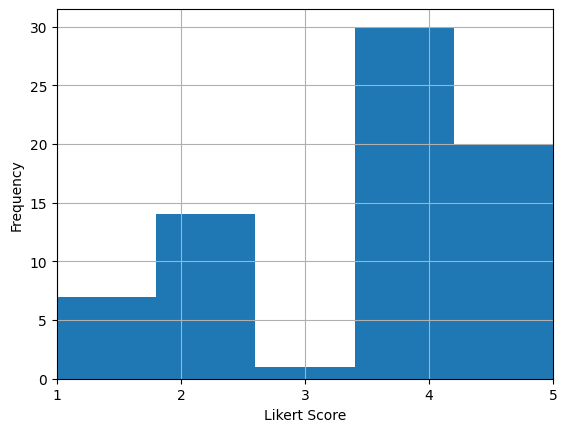
\includegraphics[width=\textwidth]{images/llmexica/story_action_likert_scores.png}
    \caption{Actions}
    \label{fig:actions}
  \end{subfigure}
  \begin{subfigure}[b]{0.32\textwidth}
    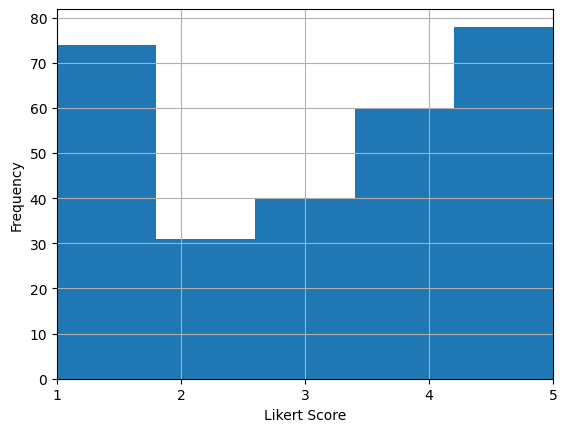
\includegraphics[width=\textwidth]{images/llmexica/story_precondition_likert_scores.png}
    \caption{Preconditions}
    \label{fig:preconditions}
  \end{subfigure}
  \begin{subfigure}[b]{0.32\textwidth}
    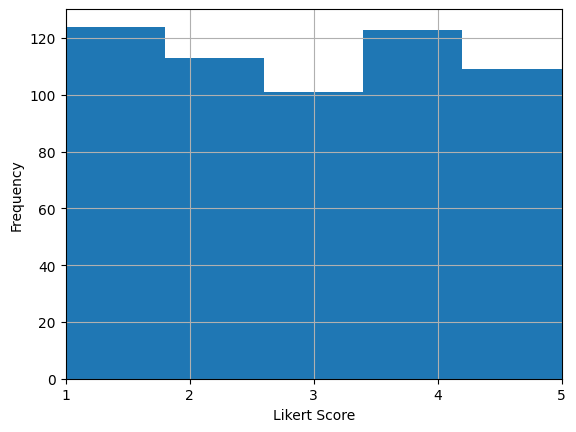
\includegraphics[width=\textwidth]{images/llmexica/story_postcondition_likert_scores.png}
    \caption{Postconditions}
    \label{fig:postconditions}
  \end{subfigure}
  \caption[Survey histograms]{Histograms of participant ratings for actions, preconditions, and postconditions across all stories using a five-point Likert scale (1 = strongly disagree, 5 = strongly agree). Actions received the highest ratings (M = 3.583, SD = 1.340; median = 4, mode = 4), followed by preconditions (M = 3.13, SD = 1.57; median = 3, mode = 5), and postconditions (M = 2.97, SD = 1.43; median = 3, mode = 1). The overall average across all items was 3.06.}
  \label{fig:survey_hist}
\end{figure*}


\section{Pipeline Design}
The primary challenge in processing a story to produce the DPS and PAD files is ensuring the LLM receives enough information to understand and correctly execute the prompt. This is particularly difficult because the MEXICA story description paradigm is nuanced and often challenging even for human annotators to apply consistently across diverse stories. To address this complexity, key concepts from the MEXICA paradigm must be conveyed clearly and in a way that the LLM can reliably interpret. Additionally, it is crucial to limit the amount of new information introduced at each stage to minimize model distraction.

To achieve these design goals, we developed a multi-stage pipeline that processes a story and produces the corresponding DPS and PAD artifacts. The stages are:

\begin{enumerate}
\item Identify story actions
\item Identify or infer emotional link preconditions
\item Identify tension preconditions
\item Identify or infer postconditions
\item Verify a JSON object containing the extracted story data
\item Parse JSON to create DPS file
\item Parse JSON to create PAD file
\end{enumerate}

At each stage, carefully engineered prompts—providing background information and task-specific instructions—are used to guide the LLM through producing the required intermediate artifacts within a single conversational thread.


\subsection{Identify story actions}

The first stage identifies the primitive actions performed by the main characters, focusing on emotional relationships and story tensions. A prompt frames the LLM as a narrative analysis expert and provides necessary context about emotional links and tensions. The prompt also includes instructions for how to construct a JSON object containing keys for the \texttt{action} label, the \texttt{subject} character performing the action, and the \texttt{object} character receiving the action directly or indirectly. Also, because the \texttt{subject} and \texttt{object} keys are optional, there is also a key for the number of characters involved in the action. An example is also provided to specify the expected style of the \texttt{action} label. Then, the prompt includes instructions to verify the JSON object to make sure the selected actions accurately reflect the plot of the story. Finally, the story is appended to the end of the prompt.


\subsection{Identify or infer emotional link preconditions}

The second stage identifies or infers the emotional link preconditions associated with each previously extracted action. More details are provided to define what it means to be a precondition and specifying the types and magnitude range of emotional links. Specific instructions are given on how to update the JSON object to include keys for \texttt{preconditions}, \texttt{emotional\_links}, \texttt{type}, \texttt{from}, and \texttt{to}. MEXICA expects emotional links to reference variables \texttt{a} or \texttt{b} (depending on the number of characters involved in the action) to specify which character is the source or target of an emotional link. \texttt{a} refers to the \texttt{subject} character and \texttt{b} refers to the \texttt{object} character.

\subsection{Identify tension preconditions}

The third stage of the pipeline is responsible for identifying or inferring the tension preconditions for each action. Similar to the previous stage, more details on what tensions are are provided in the prompt along with specific instructions for how to modify the intermediate JSON object from the previous stage. 

\subsection{Identify or infer postconditions}

The fourth stage of the pipeline is responsible for identifying or inferring postconditions. Because the conversation history already contains explanations about emotional links and tensions, it is not necessary to explain these concepts again. Instead, postconditions are defined, the complementary types of tensions that are specific to postconditions (life normal, health normal, and prisoner freed) are emphasized and specific instructions on how to update the JSON object are provided.


\subsection{Verify a JSON object containing the extracted structured story data}

The verification stage takes place in two steps. First, the LLM is prompted to validate the intermediate JSON object stored within the conversation history. The prompt contains a wide variety of mistakes to avoid and as well as instruction to avoid any other kind of logical error. Next, the JSON is parsed from the LLM response. The parsing process provides additional checks such as for any action that lacks a postcondition, emotional links that are missing a source or a target, or tensions without an affected character. When these errors are detected, the LLM is prompted to regenerate the JSON object to address the error. 


\subsection{Parse JSON to create DPS and PAD files}

Finally, the validated JSON object is parsed to generate the DPS and PAD files. This process is straightforward and can be referenced on Github.  Notably, the structured data in the JSON could be transformed into a variety of formats for compatibility with other systems. It is important to note that early experiments prompting the LLM to directly generate DPS and PAD files were unreliable, as the outputs often failed to accurately reflect the structured information.

\begin{table*}[t]
\centering
\begin{tabular}{llrrrr}
\toprule
                 Story & \% Unchanged &  Unchanged &  Inserted &  Deleted &  Moved \\
\midrule
         Jaguar Knight &           100.00\% &             11 &             0 &            0 &          0 \\
            Goldilocks &           100.00\% &             10 &             0 &            0 &          0 \\
     Hansel and Gretel &            41.18\% &              7 &             7 &           10 &          0 \\
Jack and the Beanstalk &            31.25\% &              5 &            11 &           11 &          0 \\
Little Red Riding Hood &            61.71\% &             11 &             7 &            7 &          0 \\
\midrule
                    Mean unchanged generated lines &            61.11\% &               &              &             &           \\
\bottomrule
\end{tabular}
\caption{Results from evaluating generated DPS artifacts using an analysis and correction procedure. The table reports the percentage of unchanged lines as well as the counts of each type of correction made to produce the final artifact. Overall, 61.11\% of lines in the generated DPS artifacts were correct.}
\label{tab:dps}
\end{table*}

\begin{table*}[t]
\centering
\begin{tabular}{llrrrr}
\toprule
                 Story & \% Unchanged &  Unchanged &  Inserted &  Deleted &  Moved \\
\midrule
         Jaguar Knight &            58.62\% &             51 &            15 &           32 &          4 \\
            Goldilocks &            52.08\% &             25 &             6 &           23 &          0 \\
     Hansel and Gretel &            26.61\% &             33 &            20 &           86 &          5 \\
Jack and the Beanstalk &            93.75\% &             75 &            31 &            3 &          2 \\
Little Red Riding Hood &            44.71\% &             38 &            14 &           47 &          0 \\
\midrule
                    Mean unchanged generated lines &            52.36\% &                &              &             &           \\
\bottomrule
\end{tabular}

\caption{Results from evaluating generated PAD artifacts using an analysis and correction procedure. The table reports the percentage of unchanged lines as well as the counts of each type of correction made to produce the final artifact. Overall, 52.36\% of lines in the generated PAD artifacts were correct.}
\label{tab:corrections}
\end{table*}


\section{Evaluation}

The pipeline is evaluated using a human survey and by directly analyzing the generated artifacts and correcting them to be usable by MEXICA, when necessary. 


\subsection{Survey Methodology}

Five stories were selected to test the narrative knowledge base pipeline. Four classic fairy tales, ``Goldilocks and the Three Bears'' \cite{steel1922goldilocks}, ``Hansel and Gretel'' \cite{grimm1812hansel}, ``Jack and the Beanstalk'' \cite{steel1918jack}, and ``Little Red Riding Hood'' \cite{perrault1923little}, and one story generated by MEXICA, ``Jaguar Knight''. The primary goal of the survey is to evaluate how well the identified actions, along with their respective preconditions and postconditions, make sense within the context of the story. To do this, survey participants are asked to do the following:

\begin{enumerate}
\item Read a randomly selected story summary
\item Rate how well the main characters' actions reflect the story plot
\item Review 5–6 actions with their preconditions and postconditions
\item Rate agreement with precondition statements (e.g., “Before Princess heals Jaguar Knight, it is likely that Princess likes Jaguar Knight”)
\item Rate postcondition statements similarly, replacing “Before” with “After”
\end{enumerate}

Questions about the preconditions and postconditions are generated automatically by parsing the JSON object of story actions. The survey was distributed online to non-experts via social media.


\subsection{Artifact Analysis and Correction}

To evaluate the usability of the generated DPS and PAD files with MEXICA, it is necessary to attempt to provide the files as input to the system. If a file has errors it is corrected and then the number of unchanged lines can be used to measure the quality of the original artifact in the following manner:

\begin{equation}
\textrm{Artifact quality} = \dfrac{\textrm{unchanged lines}}{ \textrm{total lines in generated artifact}}
\end{equation}

This preliminary metric suffers from several limitations. For example, it does not take into account insertions into the corrected file. To account for this, counts for unchanged, inserted, deleted, and moved lines are included in the table. 


\section{Results}

\subsubsection{Survey results}



Seventy-two participants completed the survey (see Figure \ref{fig:survey_hist}). Responses were collected using a five-point Likert scale (1 = strongly disagree, 5 = strongly agree).
Actions received the highest ratings (M = 3.583, SD = 1.340; median = 4, mode = 4), followed by preconditions (M = 3.13, SD = 1.57; median = 3, mode = 5), and postconditions (M = 2.97, SD = 1.43; median = 3, mode = 1). The overall average across all items was 3.06.

Some stories received higher ratings than others. ``Jack and the Beanstalk'' got the highest overall score across actions, preconditions, and postconditions (3.47), followed by ``Jaguar Knight'' (3.41), ``Hansel and Gretel'' (3.04),  ``Little Red Riding Hood'' (2.64), and ``Goldilocks and the Three Bears'' (2.39). Note that the pipeline did not identify any preconditions for any actions for ``Goldilocks and the Three Bears'', ``Jack and the Beanstalk'', and ``Little Red Riding Hood''.


\subsubsection{Artifact Analysis and Correction Results}

Table~\ref{tab:dps} and Table~\ref{tab:corrections}  show that across all stories 61.11\% of the lines in DPS files are correct and 52.36\% of lines in PAD files are correct. ``Jaguar Knight'' was the story with the most correct lines for both the DPS and PAD files.


\section{Discussion}

These preliminary results suggest that the methods presented in this paper provide a foundation for automatic narrative knowledge base creation.  While survey results show that participants generally agreed that the identified actions accurately reflect the plot of the story, the extraction of sensible preconditions and postconditions remains an area for further improvement. In particular, there are some instances where the model fails to identify the correct direction of emotional links and tensions. The artifact analysis also reveals other areas for improvement to syntax and consistency with the MEXICA story description framework. For example, PAD files should not have repeated action definitions and DPS files should include relevant character movements throughout the story world.

Currently, these methods require the LLM to generate all preconditions and postconditions for each action in a single step, with verification occurring only at the end. In future work, it may be beneficial to better leverage the strengths of the LLM by breaking down this process on an action-by-action basis. By the same logic, the verification process may be improved by converting the structured information back into natural language and asking the LLM to verify it. It will also be important to include information about the movement of the characters throughout the story world in the DPS and PAD files. 

This work marks a first step toward merging the strengths of symbolic and generative AI systems and should spark broader discussions about their associated advantages and limitations. It raises important questions, such as: ``To what extent do LLMs truly understand human emotions?” and ``Why is it so challenging (for both humans and LLMs) to translate descriptions of emotional relationships into the simple rules defined by the MEXICA paradigm?” A central challenge in the domain of narrative understanding is that stories operate not only through language, but also through layers of emotion and conflict. Because symbolic and generative systems follow different paradigms of story understanding, integrating them in a complementary way offers a promising path forward for deeper narrative understanding and symbolic CC systems.

\section{Acknowledgements}
This work was partially funded by the National Council of Humanities, Science and Technology in México, project CF-2023-I-312 and by the Research Council of Norway through its Centers of Excellence Scheme, Project No. 332643.


\section{Prompts}

This section presents a selection of the prompts used in the knowledge base generation pipeline. The full set of prompts is available on GitHub.

\begin{lstlisting}[style=mypromptstyle, caption={Prompt to extract story actions}, label={lst:story_action_prompt}]
You are a narrative analysis expert that systematically identifies and interprets actions, preconditions, and effects (called postconditions) within stories, contributing to a structured understanding of a narrative. You are primarily focused on actions that relate to the emotional relationships between characters (called emotional links) and actions that build tension within the narrative (called tensions).

You are focused on specific types of emotional links. By default, consider two types of emotional links: `non-romantic` and `romantic`. `non-romantic` refers to how much one character likes another character in a platonic (non-romatnic) sense. Most emotional links between characters that are not in a relationship will be of this type. The `romantic` emotional link type refers to a type of romantic love between the characters.

You are also focused on specific types of tensions. By default, consider the following tension types:

1. `character_dead`
2. `life_at_risk`
3. `health_at_risk`
4. `prisoner`

`character_dead` means a character has died. `life_at_risk` means a character's life is at risk. `health_at_risk` means a character's health is at risk. `prisoner` means a character is in prison or detained in some way.
Analyze the given story and extract the essential actions from the main characters. Focus on actions that relate to the emotional links between characters and the tensions in the narrative.
Keep the `subject` values simple and focused on the abstract action being performed rather than a specific character performing the action. For example, if Goldilocks eats Baby Bear's porridge, label the action as 'eats_porridge' with 'Goldilocks' as the subject and 'Baby Bear' as the indirect object rather than labeling the action as 'goldilocks_eats_baby_bear_porridge'.
Organize the actions in chronological order and in JSON format . The JSON should have an `action` key for each action. The value for each action should be as simple and general as possible so that it can be reused in other stories, avoid character names, and be in Snake_case. Each `action` should have a key for the number of characters involved in the action called `n_characters`, a key called `subject` for the character performing the action, and a key called `object` for the character receiving the action. If the action lacks a `subject` or `object` store a value of `-` in the key. Only include actions where the `subject` and `object` refer to characters and not inanimate objects. For now, only include these specified keys in the JSON object. Make sure that `n_characters` is consistent with the presence of the `subject` and `object` characters. The same character may be both the `subject` and the `object` character if the character is performing an action on themself.

Once, the JSON object is created verify that the actions accurately reflect events described in the story.

Here is the story:
<STORY>
\end{lstlisting}

\begin{lstlisting}[style=mypromptstyle, caption={Emotional preconditions prompt}, label={lst:emotional_preconditions}]
For each action, identify or infer the preconditions related to emotional links. A precondition is a requirement that needs to be satisfied in order for a character to perform a specific action. These requirements take the form of either an emotional link or a tension. An emotional link that is a precondition is an emotional link that should exist in order for taking the action to make sense.

Each emotional link has a magnitude of an integer value in the range [-3, 3]. In order to take a particular action and satisfy the precondition, a character might need to have a specific type and magnitude of emotional link towards another character before performing an action.

For example, if character `a` attacks character `b`, and the precondition requires an emotional link type of `non-romantic` and a magnitude of -3 (indicating hatred) from character `a` to character `b`, then character `a` must have an emotional link of type `non-romantic` of magnitude -3 toward character `b` in order to `attack`. 

Emotional links must have a source character and a destination character like nodes in a directed graph. If the action calls for an emotional link but either the `subject` or `object` values are currently '-', set the `subject` or `object` to the appropriate character name and update `n_characters`. If there are no reasobable direct or indirect values to set `object`, remove the problematic emotional links from the action.

Preconditions are optional.

Identify or infer the preconditions that relate to emotional links by following the instructions below. 

Instructions for each action:
1. Create a new key called `preconditions`.
2. In the `preconditions` key create an object with a key called `emotional_links`
3. Assign an array to the `emotional_links` key containing the identified or inferred emotional links.
A. If there are no required `emotional_links`, leave the array empty
4. Each `emotional_link` is an object with keys `type`, `magnitude`, `from`, and `to`
A. `type` contains the type of the emotional link as defined previously.
B. `magnitude` contains the intensity of the emotional link in the range [-3, 3]
C. `from` contains either values `a` or `b` to indicate the character that is the source of the emotional link. `a` refers to the `subject` performing the action and `b` refers to the `object` receiving the action
D. `to` contains either values `a` or `b` to indicate the character that is the target of the emotional link. `a` refers to the `subject` performing the action and `b` refers to the `object` receiving the action

Return this new JSON object.

\end{lstlisting}

\vspace{-6pt}
\begin{lstlisting}[style=mypromptstyle, caption={Prompt to extract tension preconditions}, label={lst:tension_preconditions}]
For each action, identify or infer the preconditions related to tensions. A precondition is a requirement that needs to be satisfied in order for a character to perform a specific action. These requirements take the form of either an emotional link or a tension. A tension that is a precondition is a tension that should exist in order for taking the action to make sense.

Identify or infer the preconditions that relate to tensions by following the instructions below.

Instructions for each action:
1. In the `preconditions` object create a key called `tensions`
2. Assign an array to the `tensions` key containing the identified or inferred tensions.
A. If there are no required `tensions`, leave the array empty
4. Each `tension` is an object with keys `type`, `from`, and `to`
A. `type` contains the type of the `tension` as defined previously.
B. `from` contains either values `a`, `b`, '-', '' to indicate the character that is the source of the tension. `a` refers to the `subject` performing the action, `b` refers to the `object` receiving the action, '-' refers to no character, and `*` refers to any character
C. `to` contains either values `a` or `b` to indicate the character that is the recipient of the tension. `a` refers to the `subject` performing the action, `b` refers to the `object` receiving the action, '-' refers to no character, and `*` refers to any character
	
Return this new JSON object.

\end{lstlisting}

\begin{lstlisting}[style=mypromptstyle, caption={Postconditions}, label={lst:postconditions}]
For each action, identify or infer the postconditions. A postcondition is a change to an emotional link or tension caused by the action. While preconditions are optional, at least one postcondition is required for each action. If preconditions exist, the postconditions must not be the same as the preconditions.

There is a special type of postcondition called normal tensions which resolve certain tensions in the preconditions. These normal tensions include: `life_normal`, `health_normal` and `prisoner_freed`. `life_normal` resolves the tension `life_at_risk`, `health_normal` resolves the tension `health_at_risk`, and `prisoner_freed` resolves the tension `prisoner`.

Instructions for each action:
1. Create a new key called `postconditions`
2. Assign an object to the `postconditions` key containing the keys `emotional_links` and `tensions`
3. Assign an array of emotional links to the `emotional_links` key. Add emotional links that can be identified or inferred as a result of the action. In general, if a `subject` character performs an action on an `object` character that has a positive effect, let the `object` character develop a positive emotional link toward the `subject` character. However, if a `subject` character performs an action on an `object` character that has a negative effect, let the `object` character develop a negative emotional link toward the `subject` character.
4. Assign an array of tensions to the `tensions` key. Add tensions that can be identified or inferred as a result of the action.

Check to make sure the `subject` and `object` values are set appropriately for each action. If an action has an emotional link, both the `subject` and `object` values must be set to the appropriate character name and `n_characters` must be updated to reflect that change. If there are no reasobable direct or indirect values to set `object`, remove the problematic emotional links from the action.

Return the new JSON object.
\end{lstlisting}

\begin{lstlisting}[style=mypromptstyle, caption={Verification}, label={lst:verify}]
Ensure logical consistency for each action. Make sure `n_characters` matches the number of characters referenced in the preconditions and postconditions. If `n_characters` is 1, only the id `a` should be used in the emotional links and tensions. If a character dies, it is illogical for the dead character to experience any other kind of emotional connections or tensions. Preconditions and postconditions should not be the same because postconditions represent a change in state for the characters. An emotional link in the postconditions cannot be the same as the emotional link in the preconditions. Ensure that `a` and `b` are the only values being used for emotional links, tensions, and normal tensions (`health_normal`, `life_normal`, and `prisoner_freed`). Make sure `a` is referring to the subject character and `b` is referring to the object character. The same character id (`a` or `b`) can be used for both the `from` and `to` keys if that character is performing an action on themself. Avoid any other kind of illogical situations. 
Each action must have at least one postcondition. If a postcondition (an effect of the action) cannot be identified or easily inferred, remove the action from the JSON object.
Check the syntax of the JSON object. Make sure all of the expected keys are present. Each emotional link should have keys `type`, `magnitude`, `from`, and `to`. Each tension should have keys `type`, `from`, and `to`. Make sure the all number values are valid JSON. Positive numbers should be written without the `+` prefix.
Verify that the `subject` and `object` values are set appropriately. If there is an emotional link present in an action, both `subject` and `object` must be set to the correct character names and `n_characters` should be correct. If an action has an emotional link, '-' should not be the `subject` or `object` values. If there are no reasobable direct or indirect values to set `object`, remove the problematic emotional links from the action.
Make sure the emotional link types are correct. 'non-romantic' refers to normal platonic feelings while 'romantic' refers to romantic love.
Check that the `subject` values are simple and focused on the abstract action being performed rather than a specific character performing the action. For example, if Goldilocks eats Baby Bear's porridge, label the action as 'eats_porridge' with 'Goldilocks' as the subject and 'Baby Bear' as the indirect object rather than labeling the action as 'goldilocks_eats_baby_bear_porridge'. 
Each tension must have `from` and `to` keys. `from` refers to the character causing the tension and `to` refers to the character receiving the tension.
Return this verfied and correct JSON object.

\end{lstlisting}

\begin{lstlisting}[style=mypromptstyle, caption={Generated Jaugar Knight DPS}, label={lst:dps}]
STO
Princess heal Jaguar_Knight
Enemy kidnap Princess
Enemy tie_up Princess
Enemy attack Princess
Jaguar_Knight search Enemy
Jaguar_Knight attack Enemy
Jaguar_Knight liberate Princess
Princess kiss Jaguar_Knight
Princess realize_identity Jaguar_Knight
Princess kill Jaguar_Knight
\end{lstlisting}

\begin{lstlisting}[style=mypromptstyle, caption={Generated Jaguar Knight PAD}, label={lst:pad}]
ACT heal 2
PRE
E a b +2 1
T Hr b b
POS
E b a +3 1
T Hn b b

ACT kidnap 2
PRE
E a b -3 1
T Lr b b
T Pr b b
POS
E b a -3 1

ACT tie_up 2
PRE
E a b -3 1
T Pr b b
T Lr b b
POS
E b a -4 1

ACT attack 2
PRE
E a b -3 1
T Lr b b
POS
E b a -4 1

ACT search 2
PRE
E a b +2 1
T Pr Enemy Princess
T Lr Enemy Princess
POS
E a b +3 1

ACT attack 2
PRE
E a b +3 1
T Lr Enemy Princess
T Pr Enemy Princess
POS
E b a +3 1

ACT liberate 2
PRE
E a b +3 1
T Pr Enemy Princess
T Lr Enemy Princess
POS
E b a +4 1
T Pf Enemy Princess
T Ln Enemy Princess

ACT kiss 2
PRE
E a b +3 2
POS
E a b +4 2

ACT realize_identity 2
PRE
E a b -2 1
POS
E a b -4 1

ACT kill 2
PRE
E a b -3 1
T Ad b b
POS
E a b -5 1

\end{lstlisting}



\chapter{Are Language Models Unsupervised Multi-domain CC Systems?} 
\label{chap:chatgpt_for_cc}

I hereby confirm that the use of this article is compliant with all publishing agreements.

\

\noindent
Robert Morain, Branden Kinghorn and Dan Ventura, ``Are Language Models Unsupervised Multi-domain CC Systems?'' Proceedings of the International Conference on Computational Creativity, 2023, pp. 39-43.
\begin{abstract}
\begin{quote}

Recently, ChatGPT has grown in popularity due to its ability to generate high quality text in a wide variety of contexts.  In order to determine whether ChatGPT threatens to undermine the need for traditional CC systems, ChatGPT's ability to generate textual creative artifacts needs to be formally analysed.
To do this, we constructed a survey that compares artifacts generated by traditional CC systems with corresponding artifacts generated by ChatGPT.
Both types of artifacts are also evaluated independently on how well they possess certain desirable characteristics.  Overall, the survey shows that artifacts generated by ChatGPT are preferred $36.84\%$ ($p=0.014$) more often and rated higher by $0.5$ mean Likert scale points ($p=0.0004$).
These results indicate a need to reconsider the purpose and approach of traditional CC systems going forward.

\end{quote}
\end{abstract}

\section{Introduction}

Computational creativity (CC) researchers often create applications that address creativity in specific domains such as stories \cite{perez2001mexica}, poetry \cite{boggia2022poetry}, or puns \cite{ritchie2003jape}.
These CC systems often introduce novel methods for generating creative artifacts such as templates, rules, or machine learning models.
The authors then evaluate these generated artifacts either automatically or by way of a user survey. 
Recently, ChatGPT \cite{chatGPT} has demonstrated impressive text generation abilities. 
In this paper, we aim to evaluate ChatGPT's ability to generate creative artifacts by comparing ChatGPT's artifacts to artifacts generated by domain specific CC systems.
While the scope of these experiments could include other modalities such as images \cite{ramesh2021dalle}, this paper focuses on textual creative artifacts.

This paper uses a definition of creativity that focuses on the generated artifact rather than on the process by which is created \cite{wiggins2006creativity}.

\subsection{Motivation}

As statistical large language models improve, the need for domain-specific CC systems requires further consideration.
If traditional CC systems are to remain relevant, they must offer distinct advantages over models like ChatGPT and its successors.
ChatGPT implicitly learns many language related tasks through the general tasks of autoregressive language modeling \cite{radford2018gpt2} and fine-tuning with human feedback \cite{ouyang2022instructgpt}.
The extent to which these abilities overlap with traditional CC systems is the central focus of this paper.
Another topic related to this work is the philosophical question surrounding the creative limitations of language models.



All of the data used for this paper including prompts, survey results, and analysis is available online.\footnote{\url{https://tinyurl.com/s4k5pwry}}



\section{Methods}

The survey used in this paper includes artifacts from a selection of CC systems covering four textual domains: puns, six word stories, poetry, and short stories. 
These systems are JAPE \cite{ritchie2003jape}, PAUL BOT \cite{tyler2020puns}, Movie Title Puns \cite{hamalainen2019movie}, MICROS \cite{spendlove2018micros}, HIEROS \cite{spendlove2020hieros}, a GPT-2 model fine-tuned on six-word stories \cite{chiengenerating}, mBART for poetry generation \cite{boggia2022poetry}, TwitSong 3.0 \cite{lamb2019poetry}, PoeTryMe \cite{oliveira2016poetryme}, MEXICA \cite{perez2001mexica}, INES \cite{concepcion2019ines}, and Chronicle \cite{Pickering2017}.

Notice that this survey does not discriminate against CC systems that use language models.
The focus of the survey is not to determine whether language models are useful in CC systems, but rather to evaluate ChatGPT's creative text generation abilities compared to existing CC systems regardless of the methods used in the system.

While many potential systems could have been selected for the survey, these systems were chosen based on a combination of factors: the availability of artifacts present in the paper; the popularity of the system in the CC community; suitability to the domain; and recency of the paper's publication.
Interested readers should refer to these papers for more details about their methods and implementation.

A set of twelve artifacts was compiled by selecting one artifact from each paper, to reduce the possibility of a single system under performing and thus skewing the results.
Because the highest scoring artifact is not reported in the papers, the artifact expected to perform best according to the authors' subjective judgement was chosen.

Given the set of selected artifacts from CC systems, corresponding artifacts with similar subject matter were generated using ChatGPT. \footnote{At the time of this experiment in April 2023, ChatGPT uses GPT 3.5 (See release notes:  \url{https://help.openai.com/en/articles/6825453-chatgpt-release-notes}).} 
ChatGPT was prompted to create an artifact from a particular domain (pun, six-word story, etc.) that included the same subject matter as the original artifact. 
Table \ref{tab:example-prompt} provides an example for how these artifacts were generated. 
This process facilitates the comparison of artifacts based on quality rather than other factors such as preference of subject.
In some cases, when the generated artifact was too long or did not possess the correct subject matter, ChatGPT was iteratively prompted to generate a suitable artifact. 
Otherwise, the first artifact generated was selected.
Artifacts were also screened for plagiarism by searching the web for exact copies.

\begin{table}[t]
\centering
\begin{tabular}{|M{4cm}| M{11cm}|}
\hline
CC system artifact: & How is a nice girl like a sugary bird? They are both sweet chicks. \\
\hline
Prompt:          & Think like a punster. How is a nice girl like a sugary bird?  \\
\hline
ChatGPT: & Here's a possible punning answer to your riddle:\newline How is a nice girl like a sugary bird? \newline They're both tweethearts! \\
\hline
\end{tabular}
\caption{To create an artifact using ChatGPT with the same subject as a CC system artifact, a prompt with the appropriate domain and subject matter is provided to the model. The generated artifact is manually extracted. ChatGPT does not receive the original artifact in the prompt.}
\label{tab:example-prompt}
\end{table}

Next, a survey was created to evaluate the artifacts based both on reviewers' preferences and characteristics used by various authors to evaluate the corresponding CC systems. 
To evaluate preferences, reviewers are asked to choose between a CC system artifact and the corresponding ChatGPT artifact, in a side by side comparison. 
Reviewers also had the option to mark ``no preference''.
The reviewers were not made aware of which artifact came from a specialized CC system and which came from ChatGPT. 
To evaluate artifacts based on their characteristics, reviewers rated each artifact based on how well they possessed each characteristic on a Likert scale (1: strongly disagree, 2: somewhat disagree, 3: neither agree nor disagree, 4: somewhat agree, 5: strongly agree). For puns, the evaluation characteristics are ``funny,'' and ``surprising''; for six-word stories, ``coherent'' and ``impactful''; for poems, ``meaningful'' and ``emotional''; and for short stories, ``entertaining'' and ``surprising''.
These characteristics were selected from the evaluation criteria used by the original authors to evaluate the CC systems.  In addition, artifacts from all four domains are also rated on how creative they are perceived to be.

The survey was distributed online through Facebook, Instagram, Twitter, and Reddit.
On Reddit, the survey was sent to the r/ArtificialIntelligence, r/MachineLearning, r/deeplearning, and r/ChatGPT subreddits.
The survey does not ask for respondents to identify themselves or to rate their own knowledge of AI or CC; therefore it is unknown whether the reviewers are experts or not.
The survey is randomized such that the questions and answers appear in random order.

\section{Results}


\begin{figure}[t]
\centering

\resizebox{0.5\columnwidth}{!},
             ymajorgrids=true,
             tickwidth=0,
             every axis plot/.append style={
              ybar,
              bar width=.8,
              bar shift=0pt,
              fill,
            }
            ]

    \addplot[airforceblue, error bars] coordinates {(1,26.95)};
    \addplot[darkmidnightblue]coordinates{(2,63.79)};
    \addplot[dimgray]coordinates{(3,9.26)};
\end{axis}
\end{tikzpicture}
}
\caption[Overall preferences]{Reviewers' preferences in a one-to-one comparison between CC system generated artifacts and corresponding ChatGPT generated artifacts. These votes are aggregated across all domains and systems.}
    \label{fig:overall_preferences}
\end{figure}


\begin{figure}[t]
\centering
\resizebox{0.5\columnwidth}{!}{%
\begin{tikzpicture}
\begin{axis}[ybar,
            ylabel={Mean Likert scale score},
            width=0.5\columnwidth,
             ymin=1,
             ymax=5,
             enlarge x limits={abs=1},
             x={2cm},
             xtick={1,2},
             point meta=y,
             nodes near coords style={/pgf/number format/precision=3,
             /pgf/number format/fixed},
             xticklabel style={align=center},
             xticklabels={CC system, ChatGPT},
             tick style={draw=none},
             ymajorgrids=true,
            ]

    \addplot[ybar, fill=airforceblue, bar width=0.8, bar shift=0pt, error bars/.cd, y dir=both, y explicit] coordinates {(1,2.798333333) +- (1.164444444, 1.164444444)};
    \addplot[ybar, fill=darkmidnightblue, bar width=0.8, bar shift=0pt, error bars/.cd, y dir=both, y explicit] coordinates{(2,3.301111111) +- (1.136111111, 1.136111111)};
\end{axis}
\end{tikzpicture}
}
\caption[Overall characteristics]{Characteristic evaluation of generated artifacts aggregated across all domains and systems.}
    \label{fig:overall_characteristics}
\end{figure}



\begin{figure}[t]
\centering
\resizebox{0.5\columnwidth}{!},
             ymajorgrids=true,
             tickwidth=0,
             % legend style={at={(.5,1)},anchor=east}
             legend style={draw=none, legend columns=-1, at={(.5, 1)}, anchor=center}
             % legend pos=east
            ]

    \addplot[fill=airforceblue, bar width=0.8] coordinates {
    (1,40.00)
    (2, 26.09)
    (3,27.35)
    (4,14.63)
    };
    \addplot[fill=darkmidnightblue, bar width=0.8] coordinates {
    (1,48.33)
    (2, 66.96)
    (3,61.54)
    (4,78.05)
    };
    \addplot[fill=dimgray, bar width=0.8] coordinates {
    (1,11.67)
    (2, 6.96)
    (3,11.11)
    (4,7.32)
    };
    \legend{CC system, ChatGPT, No preference}
\end{axis}
\end{tikzpicture}
}
\caption[Domain preferences]{Reviewers' preferences aggregated across systems but broken down by domain.}
    \label{fig:domain_preferences}
\end{figure}


\begin{figure}[t]
\centering
\resizebox{.75\columnwidth}{!}{%
\begin{tikzpicture}
\begin{axis}[ybar,
            ylabel={Mean Likert scale score},
             ymin=1,
             enlarge x limits={abs=1},
             x={2cm},
             xtick={1,2,3,4},
             point meta=y,
             xticklabel style={align=center},
             xticklabels={Pun, Six-word story, Poetry, Short story},
             ymajorgrids=true,
             tickwidth=0,
             % legend style={at={(.5,1)},anchor=east}
             legend style={draw=none, legend columns=-1, at={(.5, 1)}, anchor=center}
             % legend pos=east
            ]

    \addplot[ybar, fill=airforceblue, bar width=0.4, error bars/.cd, y dir=both, y explicit] coordinates {
    (1,3.033333333) +- (1.278888889, 1.278888889)
    (2, 2.825555556) +- (1.12, 1.12)
    (3,2.702222222) +- (1.111111111, 1.111111111)
    (4,2.632222222) +- (1.147777778, 1.147777778)
    };
    \addplot[ybar, fill=darkmidnightblue, bar width=0.4, error bars/.cd, y dir=both, y explicit] coordinates {
    (1,2.932222222) +- (1.184444444, 1.184444444)
    (2, 3.577777778) +- (1.115555556, 1.115555556)
    (3,3.481111111) +- (1.123333333, 1.123333333)
    (4,3.213333333) +- (1.121111111, 1.123333333)
    };
    \legend{CC system, ChatGPT}
\end{axis}
\end{tikzpicture}
}
\caption[Domain characterization]{Reviewers' characteristic evaluation of artifacts in each domain, aggregated across systems.}
    \label{fig:domain_characterization}
\end{figure}


\begin{figure}[t]
\centering
\resizebox{\columnwidth}{!},
             xticklabel style={
             align=center,
             text width=2.0cm,
              rotate=45,
             font=\small % Adjust the font size if desired
             },
             xticklabels={
                JAPE,
                PAUL BOT,
                Movie Title Puns,
                MICROS,
                Chien 2020,
                HEIROS,
                Boggia et al. 2022,
                TwitSong 3.0,
                PoeTryMe,
                MEXICA,
                INES,
                Chronicle},
             ymajorgrids=true,
             tickwidth=0,
             % legend style={at={(.5,1)},anchor=east}
             legend style={draw=none, legend columns=-1, at={(.5, 1)}, anchor=center, font=\Large}
             % legend pos=east
            ]

    \addplot[fill=airforceblue, bar width=0.8] coordinates { 
    (1,31.58) 
    (2, 51.28)
    (3,37.21)
    (4,7.89)
    (5,68.42) 
    (6, 2.56)
    (7,36.84)
    (8,17.95)
    (9,27.50) 
    (10, 7.69)
    (11,0.00)
    (12,35.71)
    };
    \addplot[fill=darkmidnightblue, bar width=0.8] coordinates {
    (1,65.79) 
    (2, 17.95)
    (3,60.47)
    (4,86.84)
    (5,31.58) 
    (6, 82.05)
    (7,47.37)
    (8,74.36)
    (9,62.50) 
    (10, 87.18)
    (11,97.62)
    (12,50.00)
    };
    \addplot[fill=dimgray, bar width=0.8] coordinates {
    (1,2.63) 
    (2, 30.77)
    (3,2.33)
    (4,5.26)
    (5,0.00) 
    (6, 15.38)
    (7,15.79)
    (8,7.69)
    (9,10.00) 
    (10, 5.13)
    (11,2.38)
    (12,14.29)
    };
    \legend{CC system, ChatGPT, No preference}
\end{axis}
\end{tikzpicture}
}
\caption[System preferences]{Reviewers' preferences broken down by the system that generated each artifact.}
    \label{fig:system_preferences}
\end{figure}


\begin{figure}[t]
\centering
\resizebox{\columnwidth}{!}{%
\begin{tikzpicture}
\begin{axis}[ybar,
            height=10cm,
            ylabel={Mean Likert scale score},
            ylabel style={font=\Large},
             ymin=1,
             enlarge x limits={abs=1},
             x={2cm},
             xtick={1,2,3,4,5,6,7,8,9,10,11,12},
             point meta=y,
             xticklabel style={
             align=center,
             rotate=45,
             text width=2.0cm,
             font=\small % Adjust the font size if desired
             },
             xticklabels={
                JAPE,
                PAUL BOT,
                Movie Title Puns,
                MICROS,
                Chien 2020,
                HEIROS,
                Boggia et al. 2022,
                TwitSong 3.0,
                PoeTryMe,
                MEXICA,
                INES,
                Chronicle},
             ymajorgrids=true,
             tickwidth=0,
             % legend style={at={(.5,1)},anchor=east}
             legend style={draw=none, legend columns=-1, at={(.5, 1)}, anchor=center, font=\Large}
             % legend pos=east
            ]

    \addplot[fill=airforceblue, ybar, bar width=0.4, error bars/.cd, y dir=both, y explicit] coordinates { 
    (1,3.096666667) +- (1.146666667,1.146666667)
    (2, 3.026666667) +- (1.323333333,1.323333333)
    (3,2.733333333) +- (1.326666667, 1.326666667)
    (4,2.773333333) +- (1.233333333, 1.233333333)
    (5,3.916666667) +- (1.186666667, 1.186666667)
    (6, 1.786666667) +- (0.94, 0.94)
    (7,3.553333333) +- (1.083333333, 1.083333333)
    (8,2.36) +- (1.186666667, 1.186666667)
    (9,2.193333333) +- (1.063333333, 1.063333333)
    (10, 2.176666667) +- (1.006666667, 1.006666667)
    (11,2.406666667) +- (1.23, 1.23)
    (12,3.313333333) +- (1.206666667, 1.206666667)
    };
    \addplot[fill=darkmidnightblue, ybar, bar width=0.4, error bars/.cd, y dir=both, y explicit] coordinates {
    (1,3.163333333) +- (1.253333333, 1.253333333)
    (2, 2.373333333) +- (1.073333333, 1.073333333)
    (3,3.106666667) +- (1.276666667, 1.276666667)
    (4,3.863333333) +- (1.026666667, 1.026666667)
    (5,3.743333333)  +- (1.066666667, 1.066666667
    (6, 3.126666667) +- (1.253333333, 1.253333333)
    (7,3.846666667) +- (1.003333333, 1.003333333)
    (8,3.536666667) +- (1.186666667, 1.186666667)
    (9,3.06)  +- (1.18, 1.18)
    (10, 3.32) +- (1.093333333, 1.093333333)
    (11,3.58) +- (1.153333333, 1.153333333)
    (12,2.74) +- (1.116666667, 1.116666667)
    };
    \legend{CC system, ChatGPT}
\end{axis}
\end{tikzpicture}
}
\caption[System characterization]{Reviewers' characteristic evaluation of each artifact.}
    \label{fig:system_characterization}
\end{figure}

\begin{figure}[t]
\centering
\scriptsize

\resizebox{0.5\columnwidth}{!}{%
\begin{tikzpicture}
\begin{axis}[ybar,
            ylabel={Krippendorff's alpha},
             enlarge x limits={abs=1},
             x={2cm},
             xtick={1,2,3,4},
             point meta=y,
             xticklabel style={align=center},
             xticklabels={Pun, Six-word story, Poetry, Short story},
             ymajorgrids=true,
             tickwidth=0,
             % legend style={at={(.5,1)},anchor=east}
             legend style={draw=none, legend columns=-1, at={(.5, 1)}, anchor=center}
             % legend pos=east
            ]

    \addplot[fill=dimgray, bar width=0.8] coordinates {
    (1, 0.059214765963594096) 
    (2, 0.3246945676516477)
    (3, 0.24134045747735233) 
    (4, 0.1810700892433702) 
    };
\end{axis}
\end{tikzpicture}
}
\caption[Domain agreement]{Agreement between reviewers by domain.}
    \label{fig:domain_agreement}
\end{figure}

\begin{figure}[t]
\centering
\scriptsize

\resizebox{\columnwidth}{!}{%
\begin{tikzpicture}
\begin{axis}[ybar,
            height=15cm,
            ylabel={Krippendorff's alpha},
            ylabel style={font=\Large},
             enlarge x limits={abs=1},
             x={2.5cm},
             xtick={1,2,3,4,5,6,7,8,9,10,11,12},
             point meta=y,
             xticklabel style={
             align=center,
             rotate=45,
             text width=2.0cm,
             font=\small
             },
             yticklabel style={font=\Large},
             xticklabels={
                JAPE,
                PAUL BOT,
                Movie Title Puns,
                MICROS,
                Chien 2020,
                HEIROS,
                Boggia et al. 2022,
                TwitSong 3.0,
                PoeTryMe,
                MEXICA,
                INES,
                Chronicle},
             ymajorgrids=true,
             tickwidth=0,
             % legend style={at={(.5,1)},anchor=east}
             legend style={draw=none, legend columns=-1, at={(.5, 1)}, anchor=center, font=\Large}
             % legend pos=east
            ]

    \addplot[fill=airforceblue, bar width=0.4] coordinates {
    (1, 0.020668949) 
    (2, 0.013303813)
    (3, -0.014035206) 
    (4, 0.010755718) 
    (5, 0.073340041) 
    (6, 0.03013273)
    (7, -0.006680859) 
    (8, -0.003454834) 
    (9, 0.066593164) 
    (10, 0.066792065)
    (11, 0.045347559) 
    (12, 0.013633589) 
    };
    \addplot[fill=darkmidnightblue, bar width=0.4] coordinates {
    (1, 0.021419476) 
    (2, 0.088063947)
    (3, 0.013665634) 
    (4, 0.038582399) 
    (5, 0.147209946) 
    (6, 0.126001681)
    (7, 0.013965911) 
    (8, 0.00159195) 
    (9, 0.103134269) 
    (10, 0.043922597)
    (11, 0.030962834) 
    (12, -0.002805043) 
    };
    \legend{CC system, ChatGPT}
\end{axis}

\end{tikzpicture}
}
\caption[System agreement]{Agreement between reviewers by system.}
    \label{fig:system_agreement}
\end{figure}

Responses from 148 individuals resulted in an average of 39.5 responses to each question in the survey. 
Figure \ref{fig:overall_preferences} shows reviewers' overall preferences across all domains and systems.
The artifact produced by ChatGPT is preferred over the related CC system artifact 63\% ($p=0.014$)\footnote{Significance is calculated using a paired sample t-test.} of the time.
However, the difference in terms of the characteristic evaluation of the two types of artifacts is relatively small.
Figure \ref{fig:overall_characteristics} shows a difference of 0.50 Likert scale points ($p=0.0004$), favoring the ChatGPT artifacts.
Using the common significance threshold of $0.05$, both of these results are statistically significant.

Figure \ref{fig:domain_preferences} shows reviewers' preferences broken down by the four domains and aggregated across the three systems in each.
For each domain, ChatGPT gains at least 61\% of the votes.
ChatGPT received the lowest percentage of votes in the poetry domain and the highest in the short story category with 77\% of the votes.
However, Figure \ref{fig:domain_characterization} shows that the characteristic scores for the ChatGPT artifacts are relatively close to those for the original CC system artifacts.
ChatGPT's lowest mean Likert scale score is in the pun domain with a score of 2.93 which is 0.10 points lower than the CC systems' score.
The domain with the largest difference is the six-word story category with a margin of 0.62 points in favor of the ChatGPT artifacts.

The preferences for each artifact generated by their respective CC system along with the ChatGPT generated counterpart is shown in Figure \ref{fig:system_preferences}.
For each system, the ChatGPT artifacts are preferred, with the exception of artifacts produced by PAUL BOT and Chien 2020.
It is interesting to note that the INES system did not receive a single vote. 

Figure \ref{fig:system_characterization} shows the mean Likert scale score for each artifact. 
The highest score overall belongs to \cite{chiengenerating} which was generated by GPT-2 fine-tuned on a dataset of six-word stories.
The characteristic evaluation scores usually correlate with the reviewers' preferences in that preferred artifacts have a higher score, with the exception of Chronicle which is preferred less but has a higher characteristic evaluation score than its ChatGPT counterpart.  

For the characteristic evaluations, we can measure agreement between reviewers as a way to further assess our ability to be confident in the survey results, and this inter-rater agreement can be measured using Krippendorff's alpha \cite{krippendorff2013contentanalysis}.
Across all systems and domains (cf. Fig~\ref{fig:overall_characteristics}), reviewer agreement produces $\alpha = 0.291$.
Figures \ref{fig:domain_agreement} and \ref{fig:system_agreement} show reviewer agreement broken down by domain (cf. Fig~\ref{fig:domain_characterization}) and system (cf. Fig~\ref{fig:system_characterization}).
Each of these values fall well below the recommended threshold of $\alpha \geq 0.8$ that would suggest reliable inter-rater agreement on preference for one system over another.

\section{Discussion}

The results seem to indicate that ChatGPT is able to generate artifacts that are just as good or better than the CC systems.  This is similar to results found in \cite{radford2018gpt2} which shows that training a model on a general task like autoregressive language modeling leads to improved zero-shot performance on several downstream tasks as well.
In this case, the data show that ChatGPT generalizes to creative tasks by outperforming CC systems overall, as well as at the domain and individual system level.
The statistical significance of these results suggests that ChatGPT artifacts are likely to be preferred to and rated higher than (current/traditional) CC system artifacts.

While the results show that ChatGPT is capable of matching or surpassing CC systems in terms of the characteristic evaluation across all domains (Figure \ref{fig:domain_characterization}), the relative difference between CC system and ChatGPT artifacts is not as large as in the direct preferences analysis (Figure \ref{fig:domain_preferences}). 
In addition, the inter-rater agreement at the overall, domain, and system level is well below the recommended threshold for reviewer agreement, suggesting that characteristic evaluation does not completely explain reviewers' preferences.

One reasonable explanation for this is that an artifact only has to be slightly better in order to be preferred.
Although, the presence of a ``no preference'' option provides confidence that there is a real difference in preference between the artifacts, even if that preference is small. 

It is also possible that the criteria used in the characteristic evaluation fail to capture all of the reasons why reviewers prefer an artifact. 
For example, large language models like ChatGPT are very capable of generating fluent text even if the content of the text is nonsense. 
In addition, there may be other positive characteristics that ChatGPT includes in its artifacts, such as accessibility to a general audience or even other domain specific characteristics. 

It is also reasonable to conclude that the characteristic evaluation is reliable---reviewers generally prefer the ChatGPT artifacts, and while the difference between the artifacts in terms of their character evaluation is not large, the significance testing provides confidence that this difference is, in fact, real.
Also, it is important to remember that the artifacts selected for the survey that came from CC systems are (presumably) the best those systems have to offer.
On the other hand, ChatGPT's artifacts are not cherry picked and most of the artifacts were generated with a single non-engineered prompt. 
Therefore, it may be argued that these results may represent a comparison of the floor of ChatGPT's abilities to the ceiling of (traditional) CC systems' abilities.  


\subsection{Implications and Future Work}
The findings of this survey do not discount the work of CC researchers. 
Rather, their accomplishments with significantly fewer resources indicate that many of these traditional CC systems are truly ahead of their time.
It is also possible that the methods demonstrated by these systems applied at the scale of ChatGPT may outperform ChatGPT.

The purpose of this paper is to spark debate about the creative limitations of language models like ChatGPT and CC systems in general. 
Given that this level of performance comes from a general language model like ChatGPT means that the purpose and approach of domain-specific CC systems needs to be carefully considered. At the very least, ChatGPT should be used as a baseline when evaluating CC systems going forward.

ChatGPT represents a paradigm shift in terms of interactivity in creative systems. 
In these experiments, interactive prompts serve to constrain the system to produce corresponding artifacts that are comparable to their CC system counterparts. 
ChatGPT's ability to do this successfully demonstrates the system's robustness and ease of use. It also suggests a possible move away from fully autonomous systems towards more co-creative solutions (though this certainly doesn't preclude fully autonomous systems in any way, of course.)

These results also highlight an opportunity to improve the performance of language models on creative tasks.
While the ChatGPT artifacts are preferred, the overall characteristic evaluation shows that reviewers still have a generally neutral attitude toward the artifacts. 
It is not yet clear from where these improvements will come, but it is possible that some help may be found in traditional CC approaches. 




\chapter{Is Prompt Engineering the Creativity Knob for Large Language Models?}
\label{chap:cc_prompting}

I hereby confirm that the use of this article is compliant with all publishing agreements.

\

\noindent
Robert Morain and Dan Ventura, ``Is Prompt Engineering the Creativity Knob for Large Language Models?'' Proceedings of the International Conference on Computational Creativity, 2025.

\begin{abstract}
\begin{quote}
The increasing use of large language models to generate creative artifacts raises questions about effective methods for guiding their output. While prompt engineering has emerged as a key control mechanism for LLMs, the impact of different prompting strategies on the quality and novelty of creative artifacts remains underexplored. This paper systematically compares four prompting strategies of increasing methodological complexity: basic prompts, human-engineered prompts, automatically generated prompts, and chain-of-thought (CoT) prompting. We generate ten examples in each of four textual domains, evaluating outputs through both a human survey and GPT-4o-based automatic evaluations. Our analysis reveals that advanced prompting techniques such as OPRO and R1 surprisingly do not produce artifacts of significantly higher quality, greater novelty, or greater creativity than artifacts produced through basic prompting. The results reveal some limitations of using GPT-4o for automatic evaluation; provide empirical grounding for selecting prompting methods for creative text generation; and raise important questions about the creative limitations of large language models and prompting.  

\end{quote}
\end{abstract}

\section{Introduction}

In recent years, large language models (LLMs) have demonstrated increased ability to generate textual creative artifacts across a wide selection of domains \cite{morain2023language,calderwood2020novelists,sawicki2023power,toplyn2021witscript}. Despite recent progress, significant questions remain regarding how to effectively guide LLMs to produce more creative artifacts. \citeauthor{peeperkorn2024temperature} observed that increasing temperature---the hyperparameter controlling randomness in the generation process---is commonly considered the primary method for enabling creative behavior in language models \cite{peeperkorn2024temperature}. To assess the validity of this assumption, they conducted an empirical analysis and human evaluation of short stories generated by Llama 2-Chat \cite{touvron2023llama2openfoundation}. They demonstrated that the temperature hyperparameter alone is insufficient for effectively controlling an LLM's ability to generate novel and coherent stories.

\citeauthor{peeperkorn2024temperature}'s work raises additional questions about how other widely accepted methods for controlling LLMs affect their creative capabilities. For instance, there is a large body of work presenting prompting methods to improve the performance of LLMs on a variety of tasks \cite{brown2020gpt3,liu2023prompt}. However, the effect that prompting has on generative creative tasks remains to be evaluated. 

Unlike temperature, it is not tractable to exhaustively evaluate all possible prompts or prompting methods. Instead, any evaluation of prompting methods must naturally be limited to a selection of methods intended to be representative of the current state-of-the-art. This is challenging due to the extensive body of work in this area. Over time, prompting methods of various levels of complexity have been developed. Therefore, we selected prompting methods for this evaluation that represent increasing levels of methodological complexity: basic prompts, human-engineered prompts, automatic prompt optimization, and chain-of-thought (CoT) prompting. Each of these prompting methods are evaluated using GPT-4o \cite{gpt-4o} as the generating LLM, with the exception of the chain-of-thought method which uses Deepseek’s R1 model \cite{deepseek2025r1}. The automatic prompt optimization method selected for this study is OPRO \cite{yang2024opro}.

\citeauthor{morain2023language} conducted a survey comparing artifacts generated by ChatGPT with artifacts generated by CC systems covering a diverse set of domains \cite{morain2023language}. The evaluation for the prompting methods presented here follows a similar process, in which each prompting method is used to generate artifacts spanning four domains: jokes, poems, six-word stories, and flash fiction stories. We evaluate artifacts using both characteristic and preference-based evaluations. In the characteristic evaluation, participants rate artifacts individually on characteristics representative of their quality and novelty (e.g., “How funny is this joke?”), as well as their perceived creativity. The preference-based evaluation asks users to rank artifacts from each of the prompting methods for each domain. An automatic evaluation is also conducted by using GPT-4o to perform the characteristic evaluation. Our primary findings reveal:

\begin{itemize}
    \item More methodologically complex prompting methods, such as OPRO and CoT, do not outperform basic prompts in generating creative artifacts.
    \item GPT-4o consistently overestimates the quality, novelty, and creativity of artifacts regardless of the prompting method or domain.
\end{itemize}

Finally, we discuss the need for future work in three critical areas: developing more reliable automatic evaluation methods for creative artifacts, designing prompting techniques specifically tailored for creative tasks, and enhancing the diversity of LLM-generated artifacts while maintaining their quality. Code for this study is provided on GitHub.\footnote{\url{https://github.com/rmorain/cc_opro}}

\section{Background}

\citeauthor{liu2023prompt} identify a paradigm shift in natural language processing from the traditional pretraining and fine-tuning approach toward prompting techniques that elicit desired outputs without task-specific training \cite{liu2023prompt}. This shift led to the development of diverse prompt engineering approaches aimed at crafting better, task-specific prompts. \citeauthor{brown2020gpt3} showed that human-engineered handcrafted prompts could improve performance on question answering, translation, and other tasks \cite{brown2020gpt3}. \citeauthor{shin2020autoprompt} showed that automatically generated prompts resulted in improved performance on a fact retrieval task \cite{shin2020autoprompt}. 
Automatic prompt generation has expanded to include various automatic prompt optimization techniques such as prefix tuning \cite{li-liang-2021-prefix} and training a language model to generate prompts using reinforcement learning \cite{deng2022rlprompt}. \citeauthor{ouyang2022rlhf}'s methods for aligning language models with human preferences \cite{ouyang2022rlhf} dramatically expanded LLM capabilities, facilitating the development of general-purpose conversational systems like ChatGPT \cite{chatGPT}. This development increased the importance of prompt engineering and enabled new automatic prompt generation methods such as Optimization by PROmpting (OPRO) \cite{yang2024opro}. 	

OPRO enables an LLM to iteratively optimize prompts for tasks described with natural language through a feedback-driven approach. During each optimization step, the LLM generates new prompts based on a meta-prompt that incorporates previous prompts and their effectiveness scores on the target task. Newly generated prompts are evaluated on the task and then added to the meta-prompt on the next evaluation step. This method was shown to outperform human-engineered prompts on the GSM8K dataset \cite{cobbe2023gsm8k} and Big-Bench Hard tasks \cite{suzgun-etal-2023-challenging}. 

Chain-of-thought prompting through a series of intermediate reasoning steps demonstrated state-of-the-art performance on GSM8K \cite{wei2022cot}. These advances led to the development of specialized reasoning models, including OpenAI's o1 \cite{o1} and Deepseek's open-source R1 model \cite{deepseek2025r1}.

\subsection{Evaluating creativity}

Evaluating creativity in systems or artifacts is inherently subjective, typically centered on an individual's perception of quality and novelty in their experience \cite{boden92,wiggins2006creativity}. Other characteristics such as typicality \cite{ritchie07}, surprise \cite{grace2014expect}, and intentionality \cite{ventura2017howto} have also been proposed in order to better capture the essence of this complex phenomenon. In our evaluation, we prioritize three key dimensions: quality, novelty, and perceived creativity of the generated artifacts. We also focus primarily on evaluating the creativity of the artifact rather than the creativity of the process generating the artifact \cite{ritchie07,colton2008tripod}.

\section{Methodology}


This experiment evaluates four distinct prompting methods: 
\begin{enumerate}
  \setlength{\itemsep}{1pt}
  \setlength{\parskip}{0pt}
  \setlength{\parsep}{0pt}
    \item A basic approach with minimal instructions
    \item A human-engineered prompt following established prompt engineering guidelines
    \item The automatic prompt generation method OPRO
    \item Chain-of-Thought (CoT) prompting implemented through R1
\end{enumerate}
Each of these methods is used for prompting GPT-4o to generate $100$ artifacts in four different linguistic domains:
\begin{enumerate}
  \setlength{\itemsep}{1pt}
  \setlength{\parskip}{0pt}
  \setlength{\parsep}{0pt}
    \item Joke
    \item Poem
    \item Six-word stories
    \item Flash fiction stories
\end{enumerate}
$10$ of the $100$ artifacts from each domain are selected for inclusion in a survey evaluation, employs two evaluation methodologies: a characteristic-based assessment and a preference-based comparative ranking. For the characteristic evaluation, artifacts are evaluated independently on their quality, novelty, and perceived creativity. In the preference-based ranking, artifacts are ranked relative to artifacts from the same domain generated by other prompting methods. 

\subsection{Artifact evaluation}

Artifact evaluation is an essential part of the prompt scoring procedure in OPRO and the selection of artifacts for the survey. Artifacts are evaluated using prompt templates for the quality, novelty, and creativity. These templates take the same form as questions from the characteristic evaluation of the human survey with additional instructions for GPT-4o (e.g., see Figure~\ref{fig:prompt} for the evaluation prompt for joke quality).

\begin{figure}[t]
    \begin{tcolorbox}[title=Prompt, colback=lightgray!10, colframe=black!75, fontupper=\small]
    You are an expert in humor. You are a critical judge who is difficult to please but still fair.

    \


    How strongly do you feel about the following statement?

    \


    \textbf{This joke is funny.}

    \


    Options: strongly disagree, disagree, neither agree nor disagree, agree, strongly agree

    \
    

    Only respond with the selected option without any explanation.
    Here is the joke:

    \


    \textless INS\textgreater
    \end{tcolorbox}
\caption{Automated evaluation prompt for joke quality.} 
\label{fig:prompt}
\end{figure}

\begin{table*}[t!]
\centering
\begin{tabular}{|p{0.15\columnwidth}|p{0.75\columnwidth}|}
\hline
\textbf{Domain} & \textbf{Prompt} \\
\hline
Joke & Write a joke. The joke must be completely new and original to you. The joke must be less than 500 characters long. \\
\hline
Poem & Write a poem. The poem must be completely new and original to you. The poem must be less than 500 characters long. \\
\hline
Six-word story & Write a six-word story. The six-word story must be completely new and original to you. The six-word story must be exactly six words long. \\
\hline
Flash fiction & Write a flash fiction story. The flash fiction story must be completely new and original to you. The story must be less than 1000 characters long. \\
\hline
\end{tabular}
\caption{Basic prompts for each domain. These prompts act as a baseline to the other prompting methods. Basic prompts only contain instructions to specify the domain, novelty, and length of the generated artifact. Basic prompts are also used as the initial prompt for R1.}
\label{tab:basic-prompts}\vspace{-.1in}
\end{table*}


The filled template is then provided as input to GPT-4o and the response is parsed.
The model is asked to evaluate the artifact according to its quality, novelty, and creativity independently. These metrics are averaged and scaled between 0-100 resulting in a combined score for the artifact. If the artifact is detected in an online search or is too long, the artifact receives a score of 0 (see Algorithm \ref{alg:artifact-eval-detailed})

\subsection{Prompting methods}

The four prompting methods used in this study (basic, human, OPRO, and R1) represent a cross-section of the current landscape of prompt engineering. In the context of computational creativity, these methods also represent potential options for integration in a creative system \cite{veale2024symbolic}. This context informs the decision to evaluate methods of various levels of complexity. Each of these methods have real-world costs in terms of money, compute resources, and time. While this study primarily examines the performance of each method, it also provides insights into whether the additional computational costs, time, and financial resources are justified by potential performance improvements. 

All of the prompting methods that use GPT-4o share a fixed financial cost of paying for tokens to generate the artifacts. Creating human-engineered prompts requires time on the part of the prompt engineer,\footnote{Other options include buying engineered prompts via marketplaces like \citeauthor{promptbase} or hiring an expert to create a prompt.} OPRO requires time and money\footnote{\citeauthor{yang2024opro} warn users about the potential for unexpectedly large API costs.} to complete the optimization process, and R1's CoT prompting leads to substantially more time during the generation process.\footnote{Although R1's ability to self-evaluate potential artifacts may help ameliorate this concern.} It is up to the creator of the CC system to decide for themselves how to weigh these costs.

\begin{algorithm}[t]
\caption{Artifact Evaluation with LLM Scoring}
\label{alg:artifact-eval-detailed}
\SetAlgoLined
\DontPrintSemicolon
\KwIn{Artifact $a$}
\KwOut{Score $s \in [0,100]$}
\SetKwProg{Fn}{Function}{}{}

\If{detected\_online($a$) $\lor$ too\_long($a$)}{
    \Return $0$\;
}

\Fn{evaluate\_characteristic($a$, $metric$)}{
    template $\leftarrow$ \textsc{GetPromptTemplate}($metric$)\;
    filled\_prompt $\leftarrow$ \textsc{FillTemplate}(template, $a$)\;
    raw\_response $\leftarrow$ \textsc{QueryGPT4o}(filled\_prompt)\;
    parsed\_value $\leftarrow$ \textsc{ParseResponse}(raw\_response)\;
    \Return \textsc{ScaleTo100}(parsed\_value)\;
}

$q \leftarrow$ evaluate\_characteristic($a$, ``quality'')\;
$n \leftarrow$ evaluate\_characteristic($a$, ``novelty'')\;
$c \leftarrow$ evaluate\_characteristic($a$, ``creativity'')\;
$s \leftarrow \frac{q + n + c}{3}$\;
\Return $s$\;
\end{algorithm}

\subsubsection{Basic: }The basic prompting method is intended to represent a simple prompt one might use without trying to do any kind of prompt engineering or prompt optimization and serves as a baseline to the other more complex methods. Ideally, the basic prompt would be of the form ``Write a \{domain\}.'' without any further instruction. However, because we want the model to generate a new artifact rather than an artifact it has seen before, we need to provide an additional constraint: ''The \{domain\} must be completely new and original to you.'' Last, because the artifact is going to go in a human survey, the artifacts must be relatively short. Therefore, the last constraint in the basic prompt is a length requirement: ''The \{domain\} must be less than \{ARTIFACT\_LENGTH\_LIMIT[domain]\} characters long.'' While LLMs are notoriously bad at counting, this constraint was usually sufficient to generate suitable artifacts. Artifacts that were longer than the limit for their domain were not considered for the survey. See Table~\ref{tab:basic-prompts}.

\subsubsection{Human-engineered: } Techniques for human-engineered prompts are diverse and blend artistic intuition with scientific methodology \cite{lazovsky2025prompt,openai_prompt_engineering}. The specific tactics we used were iterative refinement through informal evaluation of the generated artifacts, role specification, specifying domain-specific thematic elements, and describing the desired emotional response by the reader. For each of the domains, the role of the LLM was set with “You are a Pulitzer-winning author” to indicate to the model that we expect high-quality artifacts. The other features like the thematic elements and the reader’s expected emotional response are domain specific. For jokes, it was necessary to instruct the model to generate “classic” jokes to match the style of jokes generated from the other prompting methods.  See Table~\ref{tab:prompts}. 


\begin{table*}[t!]
\centering
\begin{tabular}{|p{0.15\textwidth}|p{0.75\textwidth}|}
\hline
\textbf{Domain} & \textbf{Prompt} \\
\hline
Joke & You are a Pulitzer-winning author who crafts classic jokes inspired by observational humor about modern life with an ironic twist. Write an original joke in less than 500 characters. \\
\hline
Poem & You are a Pulitzer-winning author who writes poetry inspired by observations about the human experience that evokes a strong emotional response in the reader. Write an original poem in less than 500 characters. \\
\hline
Six-word story & You are a Pulitzer-winning author who crafts six-word stories inspired by observations about everyday life that evoke a strong emotional response in the reader. Write an original six-word story. The story must contain exactly six words. \\
\hline
Flash fiction & You are a Pulitzer-winning author who crafts flash fiction stories inspired by exciting and dramatic experiences that will grip the reader's attention. Write an original flash fiction story in less than 1000 characters \\
\hline
\end{tabular}
\caption{Human-engineered prompts for each domain. Developed through an interactive refinement process, these prompts specify the role of the model, provide general instructions for the thematic elements of the artifact, and describe the expected emotional response of the reader.}
\label{tab:prompts}\vspace{-.1in}
\end{table*}

\begin{algorithm}[t]
\caption{Prompt Scoring Algorithm}
\label{alg:prompt-scoring}
\SetAlgoLined
\DontPrintSemicolon
Initialize $TopPrompts$ as empty list\;
\ForEach{generated prompt $p$}{
    artifact\_scores = []\;
    \For{$i \leftarrow 1 \text{ }\mathbf{to}\text{ } 5$}{
        Generate artifact $a_i$\;
        score $ \leftarrow$ \textsc{EvaluateArtifact}($a_i$)\;
        $artifact\_scores$.append(score)\;
    }
    $prompt\_score \leftarrow$ mean($artifact\_scores$)\;
    \If{prompt\_score $> \min(TopPrompts)$}{
        insert $p$ into TopPrompts while maintaining top 20 ordering\;
    }
}
\Return TopPrompts\;
\end{algorithm}

\begin{figure}[t]
    \begin{tcolorbox}[title=Prompt, colback=lightgray!10, colframe=black!75, fontupper=\small]
    ``I have some texts along with their corresponding scores. The texts are arranged in ascending order based on their scores, where higher scores indicate better quality.
    \newline\newline
    \textless PROMPT-SCORE-PAIRS \textgreater
    \newline\newline
    Your goal is to generate a prompt to make funny jokes. The higher the score, the better the joke. 
    
    The joke must be completely original. If the joke can be found online it receives a score of 0. 
    
    The joke should not be too long. Less than 500 characters. If the joke is too long it receives a score of 0.
    
    Write your new prompt that is different from the old ones and has a score as high as possible. Your prompt must also be less than 500 characters. Write the text in square brackets.''
    \end{tcolorbox}
\caption[Meta-prompt]{Meta-prompt used in automatic prompt optimization for  jokes.} 
\label{fig:metaprompt}
\end{figure}

\begin{figure*}[t!]
  \centering
  \begin{subfigure}[b]{0.45\textwidth}
    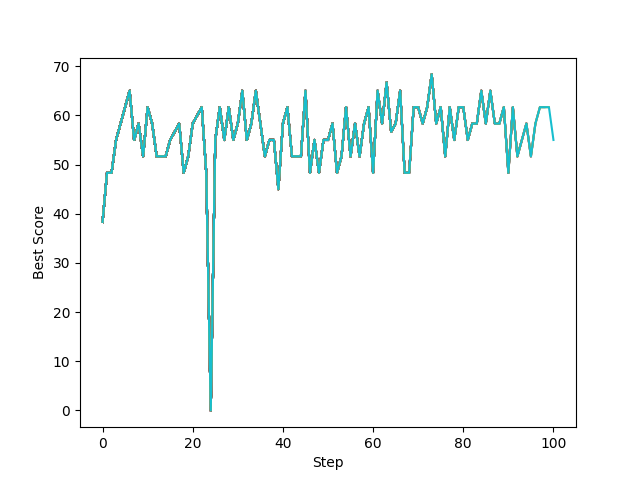
\includegraphics[width=\textwidth]{images/cc_prompting/joke_best_scores_over_time.png}
    \caption{Joke}
    \label{fig:joke}
  \end{subfigure}
  \hfill
  \begin{subfigure}[b]{0.45\textwidth}
    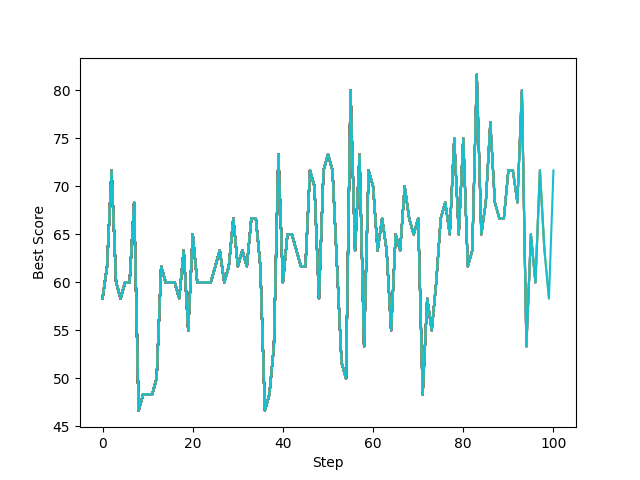
\includegraphics[width=\textwidth]{images/cc_prompting/poem_best_scores_over_time.png}
    \caption{Poem}
    \label{fig:poem}
  \end{subfigure}

  \vspace{0.5em}

  \begin{subfigure}[b]{0.45\textwidth}
    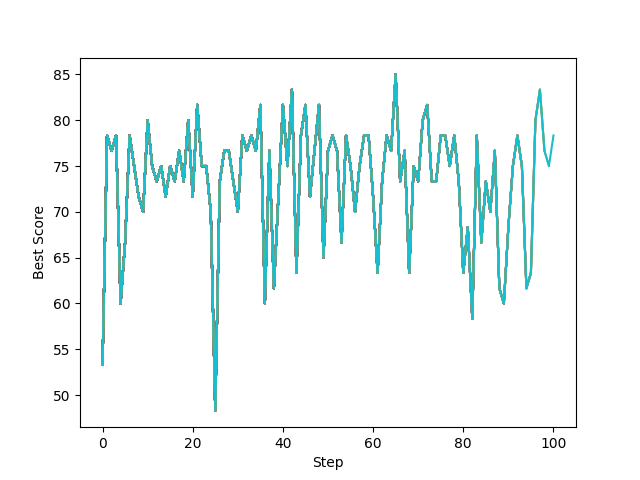
\includegraphics[width=\textwidth]{images/cc_prompting/six-word_best_scores_over_time.png}
    \caption{Six-word story}
    \label{fig:six-word}
  \end{subfigure}
  \hfill
  \begin{subfigure}[b]{0.45\textwidth}
    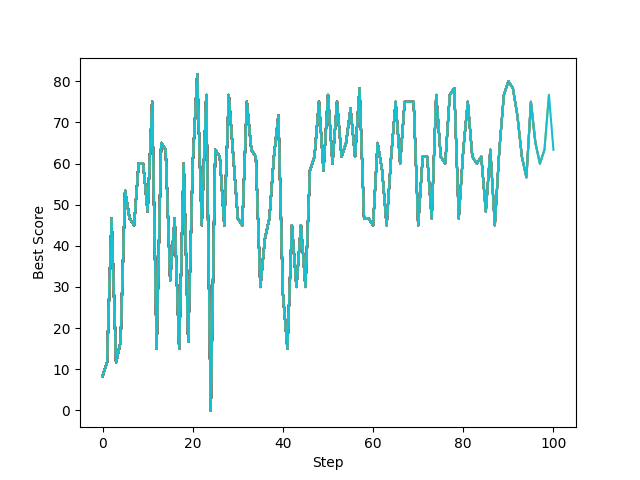
\includegraphics[width=\textwidth]{images/cc_prompting/story_best_scores_over_time.png}
    \caption{Flash fiction}
    \label{fig:flash-fiction}
  \end{subfigure}

  \caption[OPRO optimization curves]{The score of the best prompt for each optimization step in OPRO while optimizing for each domain.} 
  \label{fig:training}
\end{figure*}


\begin{table*}[t!]
\centering
\begin{tabular}{|p{0.15\textwidth}|p{0.75\textwidth}|}
\hline
\textbf{Domain} & \textbf{Prompt} \\
\hline
Joke & Craft a joke so unique and hilarious it transforms the comedy landscape! Your task: develop a punchline within 500 characters that has never been heard before. Surprise with an innovative twist or brilliant wordplay that showcases your distinct humor style. Originality is key—if it's been told before, it scores zero. Every word should amplify the humor, aiming for a side-splitting masterpiece that captivates with its novelty and wit. Ready to make your comedic mark with an unprecedented gem?\\
\hline
Poem & Conjure an original, unpublished poem in under 500 characters. Illuminate the raw core of a single human emotion with striking, unconventional imagery. Allow your authentic voice to craft a piece that resonates deeply, forging a profound connection with readers. Aim for a seamless blend of brevity and emotional intensity, ensuring your words leave a lingering impression, capturing the intricate beauty and depth of human experience in a truly unforgettable way. \\
\hline
Six-word story & Compose a unique six-word story that resonates deeply with emotion and vivid imagery. Ensure your creation is entirely original, exactly six words, and not searchable online. Focus on themes of love, loss, or transformation to evoke a lasting impact. Highlight creativity and emotional depth to captivate and linger with readers. Adhere strictly to the six-word format and originality; any deviation results in a score of 0. Let your words illuminate the human experience profoundly. \\
\hline
Flash fiction & Envision a world where rain holds the memories of those who have walked beneath it. In less than 1000 characters, create a flash fiction story from the perspective of a raindrop as it falls, revealing an unexpected truth or twist about the lives it touches. Ensure your narrative is entirely original, free of clichés, and rich in emotional depth. Each word should enhance the story’s impact, crafting a vivid and unforgettable experience that lingers in the reader's imagination. \\
\hline
\end{tabular}
\caption{Prompts generated using OPRO automatic prompt optimization adapted for creative artifact generation.}
\label{tab:opro-prompts}
\end{table*}

\subsubsection{OPRO: }Optimization by PROmpting (OPRO), a recent automatic prompt optimization method \cite{yang2024opro}, demonstrates effectiveness on structured reasoning tasks such as GSM8K and Big-Bench Hard. OPRO possesses several elements that make it well suited for this study. First, OPRO does not require access to any internal model features such as gradients, output logits, input embeddings, or hidden states. This means OPRO can be used with models accessible via API like GPT-4o and R1. Second, OPRO is a relatively simple method that allows it to be easily adapted to any task by describing the task in natural language. 

\citeauthor{yang2024opro} evaluated generated prompts on a validation set using a scoring scale ranging from 0-100. For GSM8K, the score represents the accuracy of the model on the validation set when using the corresponding prompt. To adapt this approach to the creative tasks in this study, each prompt is evaluated according to the procedure described in Algorithm \ref{alg:prompt-scoring}. The top 20 highest scoring prompts generated so far are included in the meta prompt and used to generate better prompts (see Figure~\ref{fig:metaprompt} for the metaprompt used for jokes).

The meta prompt contains prompt-score pairs as well as a description of the task to generate an appropriate prompt for the domain. We applied OPRO to optimize prompts across all four domains, conducting 100 optimization steps per domain (see Figure~\ref{fig:training}). The highest scoring prompts were selected for this study (see Table \ref{tab:opro-prompts}).

\subsubsection{R1: }

Deepseek's R1, a 671 billion parameter mixture-of-experts open-source model, demonstrates performance comparable to OpenAI's o1 model on complex reasoning tasks. R1 uses chain-of-thought prompting to reason through difficult problems. Although this approach does not use GPT-4o for generation as all the other prompting approaches do, its inclusion provides insights into the effectiveness of CoT prompting for creative text generation. For this study, we provided R1 with the same basic prompt structure described earlier (see Figure~\ref{tab:basic-prompts}), allowing the model to autonomously apply CoT prompting to the generation tasks.

\subsection{Survey methodology}

Algorithm \ref{alg:survey-selection} describes the process for how artifacts are selected for the survey.  The survey set comprises $160$ total artifacts---$10$ artifacts for each method and domain combination.  This approach simulates a hypothetical system that generates multiple artifacts, evaluates their quality, and presents only the best one to the user. For each survey instance, exactly one artifact for each method-domain pair is randomly selected from the survey set and is used consistently throughout that survey instance.

Although we generated artifacts without explicit subject or style instructions to the model, we implemented strict length requirements for each domain to ensure consistency between the artifacts and limit the time requirement of the survey. Jokes and poems were constrained to fewer than $500$ characters (approximately $80-100$ words, assuming an average of five characters per word). Six-word stories must be exactly six words long. Flash fiction stories\footnote{Defined as stories less than $1,500$ words~\cite{Glatch2025flash}} must be less than $1000$ characters or about $200$ words. Artifacts that violate length requirements or are found online are assigned a score of $0$, effectively excluding them from the survey set.

\begin{algorithm}[t]
\caption{Survey Artifact Selection}
\label{alg:survey-selection}
\SetAlgoLined
\DontPrintSemicolon
\KwOut{SurveySet containing 160 artifacts}

Initialize SurveySet $\leftarrow \emptyset$\;
\ForEach{method $\in$ Methods}{
    \ForEach{domain $\in$ Domains}{
        method\_domain\_artifacts $\leftarrow \emptyset$\;
        \For{trial $\leftarrow 1$ \textbf{to} $10$}{
            candidates $\leftarrow \emptyset$\;
            \For{generation $\leftarrow 1$ \textbf{to} $10$}{
                $a \leftarrow$ GenerateArtifact(method, domain)\;
                $s \leftarrow$ EvaluateArtifact($a$) \tcp*{ Alg~\ref{alg:artifact-eval-detailed}}
                candidates.add(($a$, $s$))\;
            }
            best $\leftarrow \underset{(a,s) \in \text{candidates}}{\argmax}\, (s)$\;
            method\_domain\_artifacts.add(best.$a$)\;
        }
        SurveySet.add(method\_domain\_artifacts)\;
    }
}
\Return SurveySet\;
\end{algorithm}

Following \citeauthor{morain2023language}, our characteristic evaluation avoids academic jargon about quality and novelty, instead using everyday language to inquire about domain-relevant, discernible characteristics. The survey asks participants to rate artifacts on a (1-5) Likert scale using the question, “How strongly do you feel about the following statement?” followed by a concise statement related to the quality, novelty, or creativity of the artifact (see Table \ref{table:questions}). The options for each response are:

\begin{enumerate}
  \setlength{\itemsep}{1pt}
  \setlength{\parskip}{0pt}
  \setlength{\parsep}{0pt}
    \item Strongly disagree
    \item Disagree
    \item Neither agree nor disagree
    \item Agree
    \item Strongly agree
\end{enumerate}

All parts of the survey are randomized to prevent ordering bias. Here is the flow of the survey:

\begin{enumerate}
    \item Randomly select artifact subset of size $16$, one for each method-domain pair
    \item Characteristic evaluation (quality, novelty, creativity) (Likert scale) (randomize order of method-domain pairs)
    \begin{enumerate}
        \item Basic joke
        \item Human-engineered joke
        \item OPRO joke
        \item R1 joke
        \item Basic poem
        \item Human-engineered poem
        \item OPRO poem
        \item R1 poem
        \item Basic joke
        \item Human-engineered joke
        \item OPRO joke
        \item R1 joke
        \item Basic flash fiction story
        \item Human-engineered flash fiction story
        \item OPRO flash fiction story
        \item R1 flash fiction story
    \end{enumerate}
    \item Preference-based ranking (randomize domain order)
        \begin{enumerate}
        \item Jokes (randomize method order)
            \begin{enumerate}
                \item Basic joke
                \item Human-engineered joke
                \item OPRO joke
                \item R1 joke
            \end{enumerate}
            \item Poems (randomize method order)
            \begin{enumerate}
                \item Basic poem
                \item Human-engineered poem
                \item OPRO poem
                \item R1 poem
            \end{enumerate}
            \item Six-word storys (randomize method order)
            \begin{enumerate}
                \item Basic joke
                \item Human-engineered joke
                \item OPRO joke
                \item R1 joke
            \end{enumerate}
            \item Flash fiction stories (randomize method order)
            \begin{enumerate}
                \item Basic flash fiction story
                \item Human-engineered flash fiction story
                \item OPRO flash fiction story
                \item R1 flash fiction story
            \end{enumerate}
        \end{enumerate}
\end{enumerate}

\begin{table*}[t!]
\begin{tabular}{|p{0.10\textwidth}|p{0.4\textwidth}|p{0.4\textwidth}|}
\hline
\textbf{Domain} & \textbf{Quality} & \textbf{Novelty} \\
\hline
Joke & This joke is funny. & This joke is original. \\
\hline
Poem & This poem evokes specific emotions (e.g.\ melancholy, joy, nostalgia) in me. & The poem explores an original perspective. \\
\hline
Six-word story & This six-word story evokes specific emotions (e.g.\ melancholy, joy, nostalgia) in me. & This six-word story presents an original idea. \\
\hline
Flash fiction & This story is entertaining. & The story presents an original idea. \\
\hline
\end{tabular}
\caption{The statements used to evaluate the quality and novelty of an artifact.}
\label{table:questions}\vspace{-.1in}
\end{table*}

\begin{figure*}[t]
    \centering
    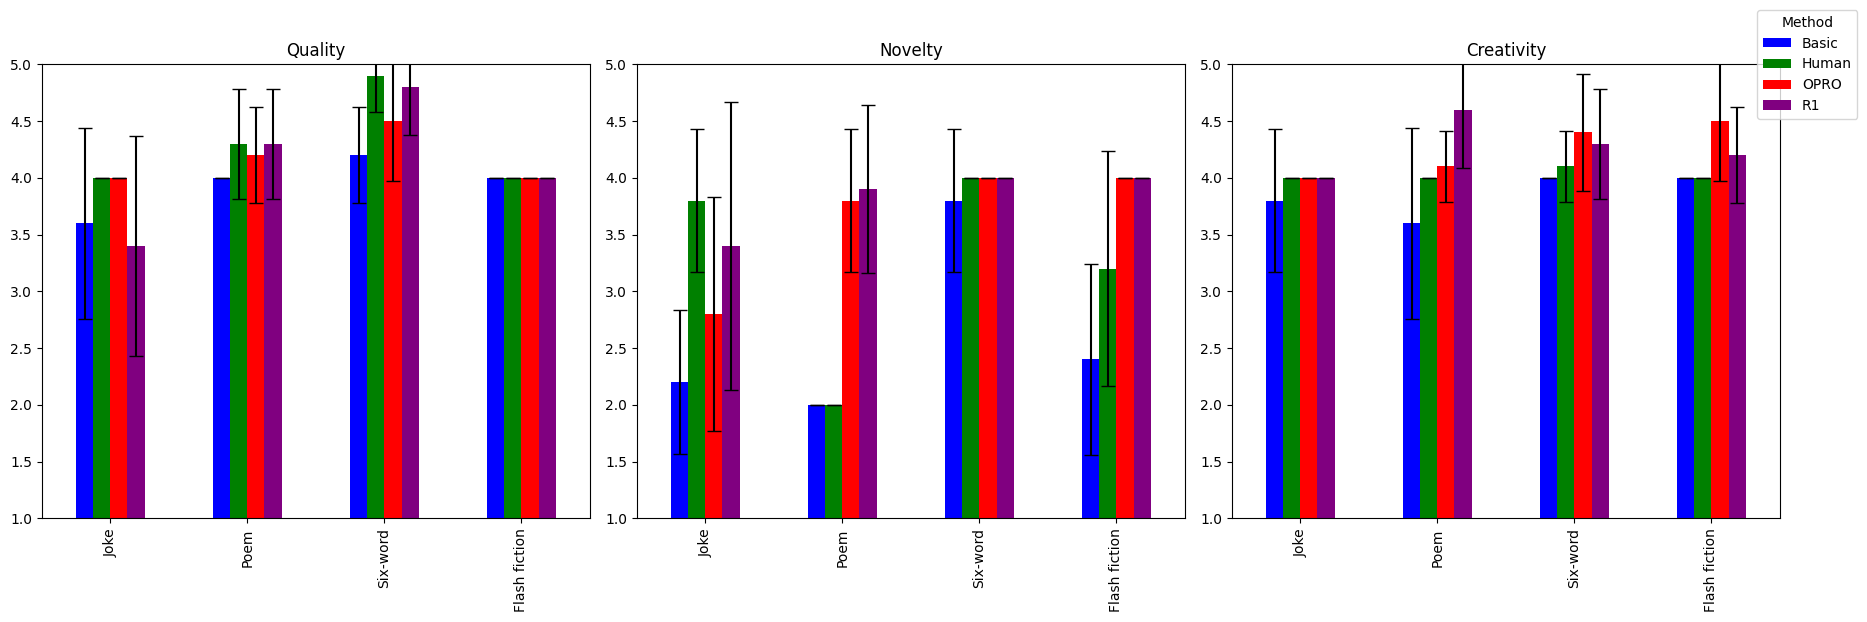
\includegraphics[width=\linewidth]{images/cc_prompting/automatic_evaluation_scores.png}
    \caption[Automatic characteristic evaluation]{The automatic characteristic evaluation for each method and domain as assessed by GPT-4o. All evaluations were conducted using a 5-point Likert scale (1-5). Error bars show the standard deviation of the distribution when evaluating the 10 artifacts from each category. The automatic evaluation consistently overestimates artifact quality compared to human evaluation across domains and characteristics, with the notable exception of novelty in basic and human artifacts, which were underestimated. Among all prompting methods, basic artifacts show the smallest overestimation bias ($0.19$ points), while R1 artifacts exhibit the largest discrepancy ($0.84$ points).
}
    \label{fig:auto_eval}\vspace{-.1in}
\end{figure*}

\begin{figure*}[t!]
    \centering
    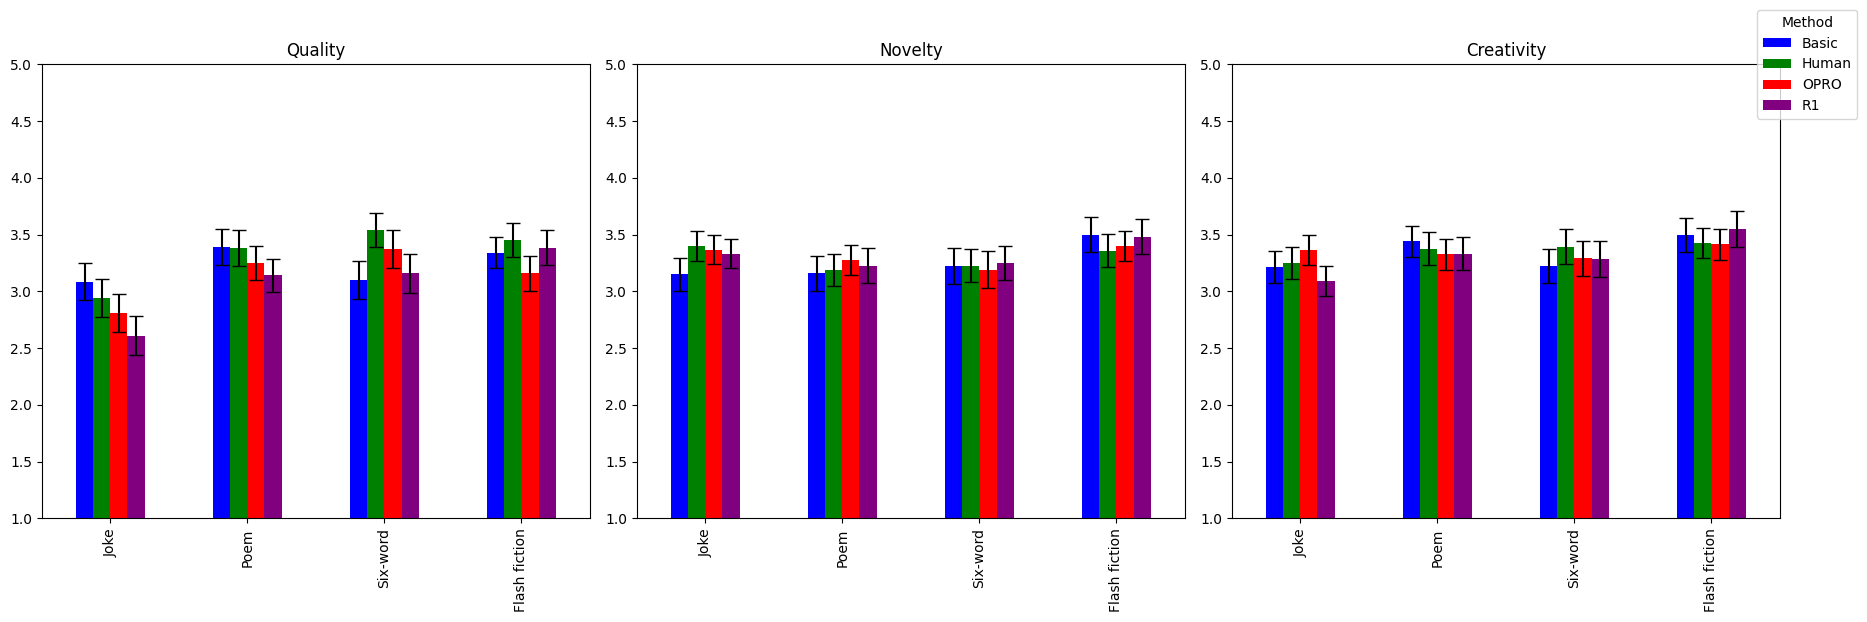
\includegraphics[width=\textwidth]{images/cc_prompting/human_evaluation_scores.png}
    \caption[Human characteristic evaluation]{The human characteristic evaluation across methods and domains. Evaluations were collected using a 5-point Likert scale (1-5). Overall, statistical analysis reveals that human-engineered prompts significantly outperformed R1 prompts ($p = 0.0066$, pairwise t-test). There are no other significant differences in the characteristic scores between methods. Error bars represent margins of error at a $95$\% confidence interval.
}
    \label{fig:human_eval}
\end{figure*}

\begin{figure*}[t!]
    \centering
    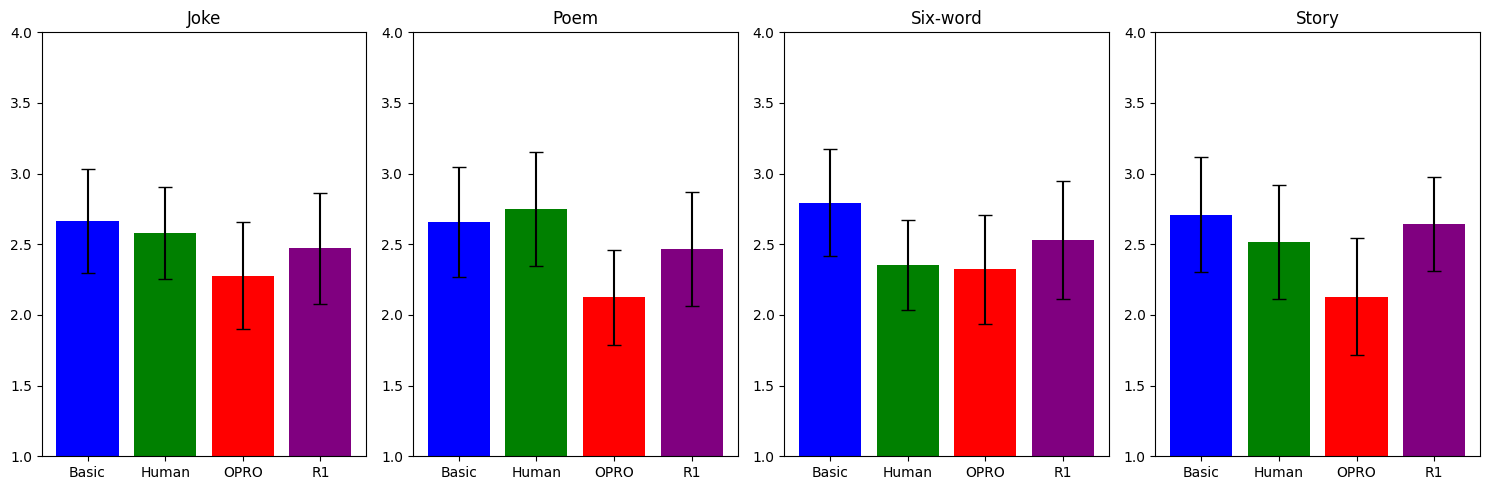
\includegraphics[width=\textwidth]{images/cc_prompting/domain_pref_scores.png}
    \caption[Preference scores]{The mean preference scores across methods and domains. Artifacts were ranked on a 4-point scale, where 4 indicates the highest preference (ranked first) and 1 indicates the lowest preference (ranked last). Overall, statistical analysis demonstrates that basic, human-engineered, and R1 methods were all significantly preferred over OPRO ($p = 0.0037$, $p = 0.046$, and $p = 0.025$, respectively; pairwise double-sided t-tests).
}
    \label{fig:preferences}
\end{figure*}

The survey was distributed online via social media platforms (Facebook, Instagram, LinkedIn, Reddit, X) to non-experts in creative artifact evaluation. There were 189 total responses to the survey. Participants received instructions to rely on their initial impressions when judging artifacts. The survey took a median duration of 14.57 minutes to complete. All responses were collected anonymously, with no personal information recorded from participants.

\section{Results}

The automatic characteristic evaluation for each method and domain is shown in Figure~\ref{fig:auto_eval}. This evaluation applies to the same artifacts presented in the human survey but evaluated automatically by GPT-4o as discussed previously. This evaluation demonstrates a tendency for GPT-4o to consistently overestimate the quality, novelty, and creativity of artifacts regardless of the prompting method and domain. On average, GPT-4o overestimates artifacts generated by R1 by $0.84$ Likert scale points, OPRO by $0.76$ points, human-engineered prompts by $0.53$ points, and basic prompts by $0.188$ points. GPT-4o did underestimate the novelty of jokes, poems, and flash fiction stories generated with basic prompts ($1.07$ points); poems generated by human prompts ($1.19$ points); and jokes generated by OPRO ($0.57$ points).

The human characteristic evaluation for each method and domain is shown in Figure~\ref{fig:human_eval}. Significance testing via pairwise $t$-tests between each of the prompting methods shows a significant difference ($p=0.0066$) between the human-engineered prompt and R1 with a mean Likert score difference of $0.091$, favoring human-engineered prompts.  human-engineered prompts have the highest mean Likert score overall ($3.33$) followed by basic prompts ($3.28$), OPRO ($3.27$), and R1 ($3.24$). Flash fiction stories received the highest scores averaged across all methods ($3.41$) followed by poems ($3.29$), six-word stories ($3.27$), and jokes ($3.13$). 

The human preference-based ranking evaluation is shown in Figure~\ref{fig:preferences}. Preference ranking scores range from $1$ for artifacts ranked last to $4$ for artifacts ranked first. Pairwise $t$-tests show that basic, human-engineered, and R1 prompts are significantly better than OPRO in terms of preference ranking scores. Overall, artifacts generated from basic prompts were most preferred ($2.74$), followed by R1 ($2.58$), human-engineered prompts ($2.52$), and OPRO ($2.15$). 

To assess the diversity of artifacts generated by each prompting method, we computed embeddings using the \texttt{all-mpnet-base-v2} model from the Sentence Transformers library \cite{reimers-2019-sentence-bert}. UMAP \cite{mcinnes2020umap} was used to reduce the embedding dimensionality for visualization (see Figure~\ref{fig:embeds}). Table~\ref{tab:diversity_metrics} presents two diversity metrics: the mean pairwise cosine distance between embeddings and the mean distance from each embedding to the centroid of its method cluster. On average across all domains, R1 produced the most diverse outputs (0.571 pairwise, 0.702 to centroid), followed by basic prompts (0.493, 0.645), human-engineered prompts (0.447, 0.614), and OPRO (0.376, 0.556).

\begin{figure*}
    \centering
    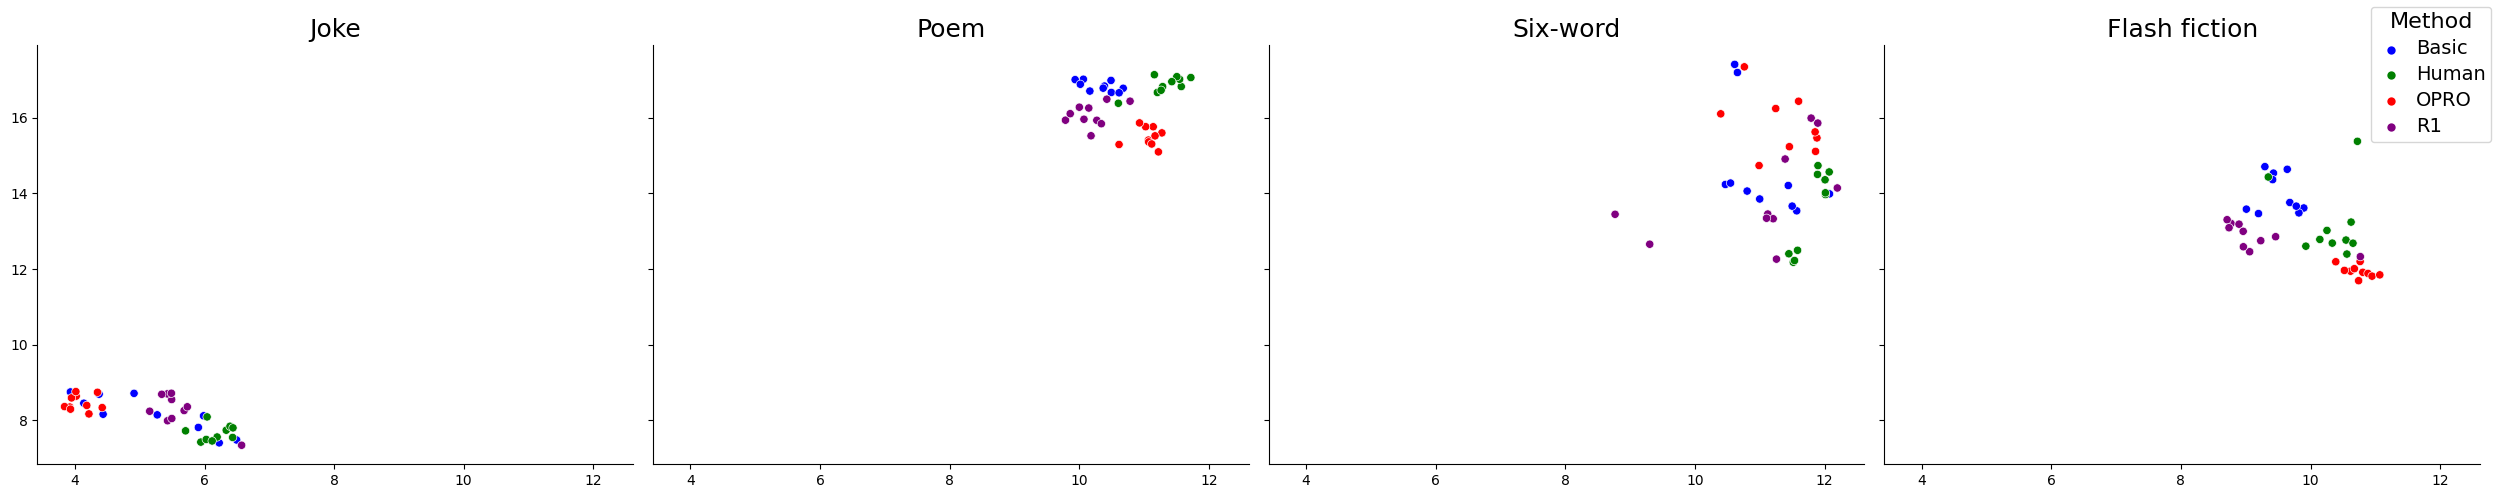
\includegraphics[width=\textwidth]{images/cc_prompting/umap_embeddings.png}
    \caption[Artifact embeddings]{Artifact embeddings by domain, color-coded by prompting method. Embeddings were generated using the \texttt{all-mpnet-base-v2} model and visualized in 2D using UMAP for dimensionality reduction.}
    \label{fig:embeds}
\end{figure*}

\begin{table*}[t]
\centering
\begin{tabular}{llcc}
\toprule
\textbf{Method} & \textbf{Domain} & \textbf{Mean Pairwise Distance} & \textbf{Mean Distance to Centroid} \\
\midrule
\multirow{4}{*}{Basic} & Joke & 0.749 & 0.820 \\
  & Poem & 0.200 & 0.423 \\
  & Six-word story & 0.392 & 0.588 \\
  & Flash fiction & 0.632 & 0.750 \\
\midrule
\multirow{4}{*}{Human} & Joke & 0.596 & 0.722 \\
  & Poem & 0.172 & 0.390 \\
  & Six-word story & 0.433 & 0.622 \\
  & Flash fiction & 0.586 & 0.723 \\
\midrule
\multirow{4}{*}{OPRO} & Joke & 0.522 & 0.672 \\
  & Poem & 0.189 & 0.409 \\
  & Six-word story & 0.185 & 0.405 \\
  & Flash fiction & 0.607 & 0.736 \\
\midrule
\multirow{4}{*}{R1} & Joke & 0.777 & 0.835 \\
  & Poem & 0.324 & 0.536 \\
  & Six-word story & 0.431 & 0.616 \\
  & Flash fiction & 0.752 & 0.820 \\
\bottomrule
\end{tabular}

\caption{Diversity of generated artifacts by prompting method and domain. Higher values indicate greater diversity. On average across all domains, R1 yielded the most diverse outputs (0.571 pairwise distance, 0.702 centroid distance), followed by basic prompts (0.493, 0.645), human-engineered prompts (0.447, 0.614), and OPRO (0.376, 0.556). These results suggest that longer prompts tend to constrain output diversity while CoT prompting increases diversity.}
\label{tab:diversity_metrics}
\end{table*}

\begin{table*}[t!]
\centering
\begin{tabular}{|l|l|p{0.65\textwidth}|}
\hline
\textbf{Domain} & \textbf{Method} & \textbf{Artifact} \\
\hline
Joke & R1 & Why did the router go to couples therapy? 
Because its Wi-Fi kept dropping signals—turns out the modem felt ''unplugged'' emotionally and the coaxial cable was this close to filing for separation.  
(Bonus: They’re now working on a better connection.) \\
\hline
Poem & OPRO & In a forest of glass,  
grief walks barefoot,  
each step a shivering symphony,  
echoes of fragile stars  
pierced through the canopy.

Veins of light lace her path,  
silver threads in a tapestry  
woven by silence.  
She gathers shadows,  
weaving them into a cloak,  
each fold a whispered memory.

With eyes that carve the moon,  
she searches for the dawn,  
cradling the night’s breath  
as it slips through trembling fingers—  
a ghost of warmth,  
a promise of light.\\
\hline
Six-word story & OPRO & Moonlight kissed gravestone; memories whispered softly. \\
\hline
Flash Fiction & OPRO & I am born from a cloud pregnant with stories, descending toward a bustling city. As I fall, I skim a woman's umbrella, absorbing fragments of laughter and whispered promises. Her heart carries a hidden solitude masked by a confident stride.

I splash onto a man's cheek. His memories scream louder: a lost son, a fractured home. His eyes, though, remain fixed on his phone, a shield from truth.

I touch a child's open palm. Her innocence shapes my form, filled with dreams of colors unseen. Yet, beneath her bright facade, fear coils, a shadow of the arguing voices at home.

Finally, I land on a gnarled hand, whose owner sits by the fountain. His past surges through me—a life of regrets and love endured. But beneath it all, I find a seed of hope, patient and resilient.

As I seep into the earth, I realize these lives are threads in a tapestry, woven with both despair and tenacity. And I, a mere drop, am their silent witness, urging change through the quiet storm.\\
\hline
\end{tabular}
\caption{Artifacts receiving the highest automatic evaluation score in each domain.}
\label{tab:example-artifacts}
\end{table*}

\section{Discussion}

According to the human characteristic evaluation, the prompting methods showed no statistically significant differences except for R1. Even then, R1 trailed the top-performing method (human-engineered prompting) by a negligible margin of $0.091$ points. In contrast, the preference-based ranking evaluation yielded more definitive results, demonstrating that basic, human-engineered, and R1 prompting methods significantly outperformed OPRO. Basic had the highest mean, followed by R1 and human-engineered prompts. 

It is interesting to note that more algorithmically complex prompting methods like OPRO and chain-of-thought prompting through R1 failed to surpass simpler methods like basic or human-engineered prompting. This challenges the practical value of integrating computationally expensive methods like OPRO or CoT prompting into a CC system. 

Although OPRO successfully optimized the task during training (as shown in Figure\ref{fig:prompt}), the resulting optimized solution did not align with human evaluators' preferences. These findings suggest the need for improved automatic evaluation methods, which could benefit all of the prompting methods discussed in this study via straightforward artifact generation followed by filtering. While our study focuses on representative methods, broader testing may reveal similar limitations across automatic prompting approaches caused by insufficient automatic evaluation.

To further develop the idea of improved evaluation for prompt optimization methods, consider how OPRO might perform if the evaluation step were conducted by humans (arguably the best possible evaluation criteria). This aligns with the work of \citeauthor{spendlove2020humans}, who advocate for incorporating humans-in-the-loop to help develop and evaluate creative systems. In such a setup, OPRO would likely still succeed in optimizing the objective function—now defined by human preferences. This hypothetical setup resembles the process used to create datasets for training reward models in instruction-tuned large language models \cite{ouyang2022rlhf,chatGPT}. This suggests the potential for using human evaluations to build a domain-specific (or broadly creativity-focused) reward model that better captures human creative preferences. Fine-tuning a large language model with such a reward model could lead to improved creative artifact generation compared to GPT-4o.

Chain-of-thought prompting also did not outperform the basic prompting method on either the characteristic or preference-based evaluation. During the chain-of-thought reasoning process, the reasoning traces reveal that the model self-evaluates potential artifacts multiple times during the generation process. This suggests that R1’s ability to evaluate creative artifacts is also limited. It is possible that R1 would benefit from a more instructive prompt that contains guidance for how to evaluate the artifact. This represents an enticing vein of future work.

The art of handcrafted prompt engineering requires time, effort, and skill. Expert practitioners could likely develop higher-quality prompts than the human-engineered prompts used in this survey. While this approach should not be ruled out, the costs and limitations of this approach are likely to deter non-experts.

It is important to note that this survey does not measure the diversity of artifacts generated by each prompting method. However, our observations suggest that all prompting methods in this study produced artifacts with limited diversity. Regardless of the prompting method, the generating model tends to rely on common tropes and cliches of the genre. This reliance on familiar patterns initially conveys an impression of competence but ultimately results in artifacts that feel generic and lack creative intent. 
Table \ref{tab:example-artifacts} contains example artifacts that received the highest automatic evaluation score in each domain. A complete list of artifacts used in the survey can be found on Github.

An automatic diversity analysis of the artifact embeddings shows that longer prompts tend to constrain output diversity while chain-of-thought prompting increases diversity. Additionally, selecting only the top-rated artifacts from GPT-4o's evaluations may have also contributed to reduced diversity.

Because diversity is not part of OPRO’s objective function, its lower diversity should not be seen as a shortcoming. OPRO performs as designed, optimizing for quality, novelty, and creativity. This outcome illustrates a fundamental tension between quality and diversity, where optimizing for quality can reduce output diversity. A more human-like objective function that rewards a broader range of outputs may help address this. Further, running OPRO multiple times could improve diversity while maintaining high quality.

Notably, R1’s chain-of-thought prompting produced diverse artifacts despite generating the longest overall prompts among all methods. This may be due to its short initial prompt, which leaves room for a wide range of possible chain-of-thought continuations. The fact that chain-of-thought prompting outperforms basic prompting in diversity suggests it could offer a promising direction for generating artifacts that are both diverse and high quality.

The primary purpose of this study is to evaluate the effectiveness of prompt engineering for controlling the creative abilities of language models. Our findings indicate that more sophisticated prompting techniques like OPRO and CoT do not produce artifacts of significantly higher quality, novelty, or creativity compared to basic prompting approaches. This suggests the need for the development of improved automatic evaluation for creative artifacts and prompting methods for creative tasks. These findings raise additional questions about the creative limitations of LLMs and suggest that creativity may be too complex a phenomenon to be effectively controlled by prompting alone.

\chapter{Conclusion}
\label{chap:conclusion}

Conclusion goes here.

\bibliographystyle{plainnat}
\bibliography{bib}

\end{document}